\documentclass{article}
% \documentclass{book}

\let\cleardoublepage\clearpage

% \setlength{\parindent}{0pt}
% \setlength{\parskip}{5.5pt}

\usepackage[english]{babel}

% Set page size and margins
% Replace `letterpaper' with `a4paper' for UK/EU standard size
\usepackage[letterpaper,top=2cm,bottom=2cm,left=3cm,right=3cm,marginparwidth=1.75cm]{geometry}
\usepackage{graphicx}
\usepackage{xcolor}
\usepackage[colorlinks=true,linkcolor=blue,citecolor=red]{hyperref}

% \setlength{\parindent}{0pt}

% \usepackage{natbib}
% \newenvironment{abstract}{}{}
\usepackage{abstract}
\usepackage{here}
\usepackage{tabularx}

\usepackage[edges]{forest}
\usepackage{tikz}
\usepackage{tikz-qtree}
\usepackage{longtable}

\hypersetup{
    colorlinks=true,
    linkcolor=[RGB]{255,34,255},
    citecolor=[RGB]{255,34,255},
}

\usepackage[whole]{bxcjkjatype}  % Japanese

\title{Notes}
\author{Shiro Takagi}
\begin{document}
\sloppy
\maketitle
\tableofcontents

\bibliographystyle{unsrt}
\bibliography{ref}

\appendix

\section{Definition}

\subsection{Alternative Definitions}
% 真理促進的ではない。帰納推論だけでは難しい。

% So far, I have examined the consequences of perceiving research as the production of new knowledge for society, and knowledge as a justified true belief. While the current definition of research may be suitable for comprehensively describing the wide range of human research conducted so far, adopting this definition led to counterintuitive conclusions with seemingly intractable problems. Therefore, I would like to discuss how this definition can be modified, or what other definitions might be conceivable.

% \subsubsection{Limited to Human Knowledge}
% One of the biggest issues of the definition is that it implies that a fully autonomous artificial researcher is likely to produce knowledge that is meaningless to humans, or even useless to understand nature. To mitigate this problem, we may force knowledge an artificial researcher produces to be relevant for humans.

% One idea is to ensure that the foundation for validation remains fundamentally human, as I mentioned above. This is because the above problem arose entirely from allowing AI to autonomously construct even the foundation for verification. It is conceivable, for example, to make AI unconditionally and strongly believe in the validity of inductive reasoning and statistical hypothesis testing 

% Another alternative is to force AI to produce knowledge that humans can understand. This is the more restrictive definition because it is conceivable that there is a procedure where humans might be convinced something is true if that is confirmed by it even if they can't fully grasp how it works. It seems that what people desire is an AI that produces knowledge in this sense, so for those people, this definition may be more than sufficient.

% A downside of adopting these definitions is that they might preclude the production of knowledge that, while certainly explaining nature, cannot be verified within the framework of human validation. If one believes that nature transcends human cognitive limitations, it seems reasonable to assume that such knowledge exists. While this may not be a concern for many people, it certainly limits the possibility of machines to do research and hence understand this nature beyond human limits. 

% It seems that one of the purposes of creating an intelligence capable of autonomously conducting research is to advance the understanding of this world beyond human limitations. Considering this, I believe that it is desirable to remove such constraints if possible. Whether such constraints are fundamentally unavoidable, or whether it is possible to relax them in some way, is something that I hope will be further discussed in the future


% \subsubsection{Knowledge Consistent with Nature}
% An approach that could be considered in principle to relax the aforementioned constraints is to enforce a verification basis that is consistent with nature, without necessarily requiring a human verification foundation. 

% As mentioned earlier, the reason humans can generate knowledge useful for understanding nature based on belief systems may be because our belief systems have been formed through interaction with nature. If this is the case, there is a possibility that by allowing machines to acquire a belief system consistent with nature in the same way, they could produce knowledge leading to the understanding of nature without being constrained by human knowledge. For instance, it might be possible, in principle, to do this by allowing machines to interact with the external world in the real world to form its belief system, just as humans do.

% However, I have no idea how to create such a machine. Even if such a machine were to be developed, as it relies on a verification basis different from humans, we might not be able to judge whether it is functioning properly. For us to be convinced of the discovery by the machine, it needs to be reflected in our belief system, but this is no different from being consistent with our belief system. Therefore, even though it is theoretically conceivable, it seems impractical to realize this approach. Considering this, it seems necessary that the basis for verification should be human one.

 
% \subsubsection{Research as New Pattern Discovery}
% One of the main reasons the definition I adopted lead to counterintuitive results may be because I regard research as the production of ``knowledge'', and knowledge as ``belief''. I interpret research as the updating of beliefs just because it is consistent with human research practices so far. Rather, an essential aspect of research seems to be discovering or creating something ``novel'', and whether or not that constitutes ``knowledge'' seems secondary.

% Given this, it might be worthwhile to simply define research as the ``discovery of new patterns (in nature)''. This definition seems to at least encompass our current research endeavors. It emphasizes the discovery of new things, is not dependent on the subject, and, (by specifying ``in nature'',) appears to align with the goal of understanding nature.

% This might be too abstract, so it would be necessary to re-analyze what this definition truly means. I'd like to consider that discussion as future work.

% \subsubsection{Research as Question Answering}
% Defining research as merely a question-and-answer process might be one approach. However, a distinguishing feature of research is that the answer is unknown to anyone. Nobody knows the correctness of the answer, but it is indirectly provided by the subject of study, such as nature. While it's unclear to what extent this formulation can alleviate the issues with the definition we've adopted, it seems worth considering for furhter study.

\subsubsection{Pragmatist Epistemology}
Up to now, we have assumed that justification should be truth-conducive since this is what most researchers would expect. That is, I regard belief that reflect the truth of this world is knowledge. However, there is also a position that regard beliefs useful for human should be knowledge. This position is known as \textit{pragmatist epistemology}. 

From this perspective, it could be possible to argue that the outputs of current machine learning models, for example, may be considered knowledge since it shows high predictive performance, leading humans to the desired behaviours. In this sense, this position is highly compatible with statistical machine learning \cite{otsuka2022thinking}.

As such, this pragmatism presents a different view of research from that of majority of researchers, and it could be seen as advocating a redefinition of the act of research. Many researchers may not accept this view. Nevertheless, in recent years, deep neural networks have made rapid advancements and have produced many ``useful'' outcomes in research, which has made the debate on whether to consider their outputs as knowledge much more relevant and realistic than ever before.

In this paper, I take the position that knowledge is JTB, and research is an endeavor to approach a truth. Therefore, I will not address this issue in the following sections that much. However, we must seriously consider the implications presented by deep neural networks and delve deeper into the discussion of how we should define research, what constitutes research, and what purpose research serves.

\section{Hypothesis Generation}

\subsubsection{How humans generate hypotheses}
One significant difference when comparing the hypothesis generation process of humans and the question-answering of machines is that the human hypothesis generation process is far more complex.


It seems that in the process of generating a hypothesis to answer a single question, humans implicitly and explicitly generate dozens or even hundreds of questions and hypotheses. As a result, in order to answer the initial question, they end up answering many different questions. Moreover, in order to generate a hypothesis, they may also test other hypotheses.


For example, Charles Darwin began with the question ``How does evolution occur?'' However, after reading Lyell's work and becoming convinced of the importance of selection in evolution as an analogy of artificial selection, he formulated and tackled the question ``How does selection (equivalent of artificial selection) occur in nature?'' Here we see a shift in the question. It was precisely because of this change in question that, upon reading Malthus's essay on population, he was able to realize that natural selection is brought about by competition between species, and thus he could fully answer the initial question, ``How does evolution occur?'' \cite{gribbin2022origin}

On the other hand, it appears that we are not having our neural networks go through such a complex process of trial and error for hypothesis generation. In many cases, when a question is presented, neural networks predict answers through a single inference based on fixed parameters. This seems too simplistic compared to the human process of hypothesis generation, which often involves repeatedly generating and testing questions and hypotheses.

% For humans, answering a question essentially means constructing the answer from known concepts. A question whose answer is unknown can be said to be one whose answer does not immediately connect with existing knowledge. Humans seem to somehow successfully link the unknown answer with their known knowledge. As these examples also illustrate, realizing the prediction of answers in cases where the answer is unknown to everyone in the world appear to be a challenge.
% 人間の場合、ある問いに答えるとは、その問いの答えを既知の概念で構成することに他なりません。答えがを知らない問いというのは、その答えが既存の知識に直ちには結びつかない問いであると言えます。このような状況下で、なんとかして答えが未知の問いを既知の知識に結びつけるのが、人間が仮説生成をする際に行なっていることであるように思われます。

% \subsubsection{Analyzing Question}
\textcolor{red}{TODO: remove or modify}
In difficult questions where the relationship to known knowledge is not immediately apparent, it seems that we first tend to analyze the question in detail. For example, let's say you have a question, ``Why are apples red?'' The first thing you would consider is what an apple is and what red means. You would also think about what it means for something to be red. Then, you would focus on the properties of apples and the color red and abstract them. you may also think about other red things besides apples. If you already know the reason why tomatoes are red before knowing why apples are red, you might consider that the reason for tomatoes being red could apply to apples as well. By conducting this kind of analysis, you can connect your understanding to existing similar knowledge and attempt to explain using those existing reasons. These ways of focusing on abstract structural similarities between specific concepts and inferring that what can be said about A, which has the same structure, can also be said about B is called \textit{analogical reasoning}. This has been considered to be important method in hypothesis generation \cite{thagard_1984}.

I believe that the process of analyzing a question corresponds to the feature transformation that occurs via the intermediate layers in a neural network. In this sense, neural networks also analyze questions. The difference may lie in the fact that humans explicitly perform the analysis of the question and ultimately make inferences for answers based on formal similarities that are linked to symbolic known knowledge.

\subsection{Generating Plausible Hypothesis}

Hypothesis generation is sometimes considered an unanalyzable, emergent process or a result of genius.\footnote{
Since 19th centuries, the act of producing knowledge, in particular hypothesis, and that of verification of it have been distinguished as the context of discovery and context of justification \cite{sep-scientific-discovery}. And during the most of the 20th centuries, the discovery caught much less attention by philosophers of science.

In engineering discussions, there is often explicit formulation of sets or candidates of hypotheses, and the discovery of hypotheses in such situations is often discussed \cite{simon1973does,kitano2021nobel,bengio2022ml4sci}. However, when automating hypothesis generation it is also important to consider how such candidates arise in the first place. There have been attempts to understand this process, such as highlighting the importance of analogy \cite{thagard1984conceptual} or mental model \cite{nersessian1999model}, but the question of how to generate ``good'' hypotheses still remains unanswered. The generation of initial hypothesis candidates has been discussed in the context of creativity in science. As you are well aware, however, current machine learning models are already capable of executing creative tasks effectively \cite{sep-creativity}. Thus, there is a debate about how much emphasis should be placed on creativity when considering the development of artificial intelligence capable of generating new hypotheses.
} However, I believe that human-generated hypotheses are produced through a process of trial and error in rational inference. In the following discussion, I will explore some examples of them.
% \footnote{
% Please note that not all research questions are why questions (e.g., ``Does life exist beyond Earth?'' is not a why question, but it is a scientifically investigable question).
% }

% \subsection{Plausible Hypothesis and Unknownness}

% While predictions that are highly unlikely to be confirmed, such as random guesses, can still qualify as research, they do not contribute much knowledge because they are expected to be easily rejected without undergoing rigorous testing. It becomes a waste of resources to invest in validating such predictions. Therefore, it seems to be crucial for ``meaningful'' research to propose hypotheses that are somewhat plausible.

% It is immediately evident that this is a non-trivial problem. This is because research, despite being an endeavor to answer unanswered questions, requires considering plausible candidate answers for those questions. Here, if the unknown under investigation is entirely unrelated to existing knowledge, it is impossible to make meaningful predictions about it. This is because predictions are based on experiences and data. In other words, high novelty and high uncertainty indicate a complex structure that cannot be immediately predicted from past knowledge and experiences. It implies that constructing plausible hypotheses necessitates the ability to discern these complex structures and patterns from past experiences. While it is difficult to determine what is unknown and what constitutes a complex structure, these can be crucial points to consider when advancing the automation of research.

\subsubsection{Analyzing Question}
Researchers start with a question, the composition of which has been discussed in the previous section. Given the question, we break down the content of the question and analyze each part in detail. For example, let's say you have a question, ``Why are apples red?'' The first thing you would consider is what an apple is and what red means. You would also think about what it means for something to be red. Then, you would focus on the properties of apples and the color red and abstract them. you may also think about other red things besides apples. If you already know the reason why tomatoes are red before knowing why apples are red, you might consider that the reason for tomatoes being red could apply to apples as well. By conducting this kind of analysis, you can connect your understanding to existing similar knowledge and attempt to explain using those existing reasons. These ways of focusing on abstract structural similarities between specific concepts and inferring that what can be said about A, which has the same structure, can also be said about B is called \textit{analogical reasoning}. This has been considered to be important method in hypothesis generation \cite{hesse1965models,thagard_1984,gentner1993shift,holyoak1996mental,dunbar1997scientists}.

For those simple examples given above, one can easily find analogical examples. However, many of the questions researchers actually grapple with are much more complex, and it's not immediately clear how they relate to existing knowledge. Even in such situations, researchers have managed to generate plausible hypotheses by thoroughly analyzing research question.

Such thorough analysis of questions seems particularly important when it comes to making significant discoveries that are remembered in history. Let's consider Charles Darwin as an example, who proposed the concept of natural selection. Darwin appears to have gone through a process of trial and error before arriving at the idea of natural selection \cite{gribbin2022origin}. After returning from his voyage on the HMS Beagle, he began to question how evolution occurs. It seems that he read the works of Lyell and Linnaeus, and particularly from Lyell's writings, he realized the importance of selection in evolution. The question then shifted to what could serve as a natural equivalent of artificial selection. Later, after reading Malthus' book on population, Darwin understood that in nature, competition leads to the preservation of advantageous species and the extinction of disadvantageous ones, which is the process of natural selection.

In essence, Darwin initially had the question of ``how does evolution occur,'' but through analyzing this question, referring to previous research, and conducting experimentations and observations, the question transformed into ``what is the equivalent of artificial selection in nature?.'' And it was through this transformation of the question that he was able to recognize the similarities between Malthus' discussion on human society and the mechanism he was seeking. Although the process is complex, this is the same as the hypothesis generation process I explained above in that he analyzed and transformed the question, finding analogies with existing knowledge and reaching a plausible hypothesis.

In the case of Darwin, it involved a more observational approach within the field of natural history, which prompted the transformation of his question. However, in fields such as theoretical research that utilize mathematics, different methods may be employed. For example, consider the scenario where there are two theories, theory A and theory B, and the goal is to achieve a unified description between them. In this case, one might repeatedly perform mathematical transformations on the objects described by each theory, reducing the significant problem of ``incompatibility between Theory A and Theory B'' to inconsistencies between specific properties of each theory. By introducing axioms that resolve these inconsistencies, it may be possible to construct a unified theory. It is important to reiterate that in cases where the subject matter is mathematically described, formal operations can be applied to objects of interest, such as object A and object B, to transform them into different forms. This process can lead to the discovery of unexpected similarities. It is through this approach that one can discuss the similarities between objects even when they may defy intuition or cannot be imagined through empirical means. 

Therefore, I believe that thorough analysis of question plays a powerful role in identifying similarities between objects, especially in cases where it is necessary to discuss the similarities between objects that may not be intuitively evident or imagined through experience. I believe that this is the core of the human hypothesis generation. The art of discovering structural similarities between two different objectives is called \textit{analogical reasoning}. This has been considered to be crucial for hypothesis generation \cite{hesse1965models,thagard_1984,gentner1993shift,holyoak1996mental,dunbar1997scientists,gentner2002analogy}. 

\subsubsection{Confirming Plausibility in Hypothesis Generation}

In the previous chapter, I explained how we transform questions by analyzing them and connecting them with existing knowledge. However, there seem to be countless ways to bring about changes in the questions. So, how exactly do we go about transforming the questions? Let's now describe the process of question transformation.

% In simple cases like ``apples are red,'' it may be sufficient to apply existing knowledge. However, in research, especially when tackling challenging questions, I believe that the following steps are involved. 

First, from the knowledge at hand, we select several hypotheses that are strongly related to the question and have a high level of confidence, and then proceed with accepting these hypotheses as premises. For example, the existing knowledge that tomatoes are red for reason A, strawberries are red for reason B  are strongly linked with the proposition that apples are red for reason C by the presence of the word ``red.'' Let's assume that you have a high level of confidence in the proposition that tomatoes are red for reason A, but only a low level of confidence in the proposition that strawberries are red for reason B. In this case, the reason A for tomatoes being red would be selected as the premise.\footnote{
In the case of humans, it may not always be the case that I prioritize knowledge with a high level of confidence. For example, let's consider a situation where I have recently read a book and acquired some highly impactful knowledge. In this scenario, even during the process of question analysis, I might be inclined to consider using this newly acquired knowledge because it has left a strong impression on us. This inclination is not solely based on its level of confidence, but rather because the knowledge has made a lasting impression, leading us to take it as a premise while analyzing the question. Like this, determining what knowledge humans choose to adopt as premises is a complex issue, and I refrain from delving into this issue in this paper.
}

Next, you will not focus on the parts of the question that pertain to the meaning of the premises or the deduced results that answer them. For example, going back to Darwin's example, when Darwin read Lyell's book, he took the proposition that ``selection matters in evolution'' as a premise. As a result, he left aside the question of ``what is important for evolution.'' Instead, he shifted his focus to solving the question of ``how does nature make selections?''

Once a certain premise is accepted, the next step involves examining the consistency between the consequences brought about by that assumption and one's existing knowledge. If introducing that premise does not lead to contradictions with strongly held beliefs, then the introduction of the premise is deemed acceptable. On the other hand, if introducing the premise results in contradictions with one's existing knowledge, it becomes a matter of choosing between the two. 

% This involves comparing the consequences brought about by the introduction of that premise with retaining one's existing knowledge and selecting the one that seems more favorable in some sense. For instance, Kepler compared the consequences of introducing the assumption of circular motion for planets with observational data and the results of his proofs, and eventually decided to discard the assumption of circular motion.

% or generating hypotheses that maintain consistency with this knowledge. Specifically, I generate hypotheses that seem relevant, and then verify that they do not contradict existing knowledge.

By considering the relationships between existing knowledge and new knowledge, and reevaluating which ones are deemed more plausible, one can undergo a process of transforming the question into its more essential form and generating plausible hypotheses. I seem to generate plausible hypothesis by transforming the question in like these steps.

\subsubsection{Continuity between Hypothesis Generation and Hypothesis Verification}

From the explanation so far, it becomes evident that in order to generate ``plausible'' hypotheses, we would conduct operations that involve changing our beliefs about the truth of those hypotheses. This seems natural since generating ``plausible'' hypotheses inherently involves such belief updates. However, this observation may offer significant insights into my current discussion. I define knowledge production as the updating of beliefs, which includes the construction of questions, the generation of hypotheses, and the operation I refer to as hypothesis testing, where I update my belief about whether a hypothesis is true. The implication of this discussion is that the process of generating ``plausible'' hypotheses and hypothesis testing share similarities. In reality, there are cases where hypothesis generation and justification are tightly connected in research practice \cite{arabatzis2006inextricability}. This leads to the question of whether we need to separate the processes of hypothesis generation and hypothesis testing.

However, I do not think that the fact that a single process play roles for both hypothesis generation and verification means that they also play the same role for knowledge production. I believe that hypothesis generation and verification play two distinct role for knowledge production, and that's why I discuss separate them as two distinct modules.

You may say that it is not entirely implausible to interpret both hypothesis generation and verification as being ``belief updates.'' Certainly, this similarity becomes more evident, particularly when contemplating the generation of ``probable'' hypotheses. For instance, let's consider a scenario where belief values are continuous. In this case, generating a hypothesis involves changing the belief value of a certain hypothesis from its original value of, say, 0 to something like 0.1. Subsequently, if multiple hypothesis candidates are considered, and one is chosen as probable based on previous research, the belief in this hypothesis might increase to around 0.3. Through the final verification of this hypothesis, the belief might reach approximately 0.9, resulting in the formation of knowledge. From this perspective, hypothesis generation and verification can be seen as the process of modifying beliefs.

However, when aiming for knowledge production within a specific society, there is a distinction. During the verification phase, the beliefs that are updated are shared beliefs. In contrast, during the generation of probable hypotheses, the updating of shared beliefs is not required. Consequently, in the context of knowledge production, hypothesis generation generates beliefs that can be updated, while hypothesis verification serves as the means to update those beliefs, thus playing distinct roles.

% \subsection{Continuity between Hypothesis Generation and Verification}
% So far, I have emphasized that hypothesis generation and hypothesis testing are functionally distinct, and that seems somewhat reasonable. However, when considering the generation of "plausible" hypotheses, these boundaries become somewhat ambiguous.

% Since testing incurs costs, in reality, humans carefully choose hypotheses worthy of testing. Even after hypothesis testing is made more efficient by machines, narrowing down hypotheses to a certain extent remains practically essential. Therefore, this is a problem that persists even after knowledge generation is achieved through machines.

% When considering the generation of ``plausible'' hypotheses, it simply means strengthening the certainty about the truth or falsehood of a hypothesis. In other words, in terms of changing the belief about the truth or falsehood of a hypothesis, this can be seen as similar to testing. For example, in experimental research, I believe there is often a pilot study conducted before starting full-scale experiments. This is nothing more than evaluating whether the hypothesis is worth pursuing for rigorous testing.

% Therefore, it may be possible to identify hypothesis generation and hypothesis testing as being synonymous in the sense of belief updating. However, I still believe that there are differences between hypothesis generation and hypothesis testing. The confidence in hypothesis generation is ultimately a matter of individual researchers or those involved in the research, and it is not necessary for all members of society to share that confidence. On the other hand, testing requires methods that update the common beliefs of members of society. Therefore, while hypothesis generation and hypothesis testing can be regarded as equivalent in terms of belief updating, they may differ in the strength of that belief.

% Obviously it is not possible to consider the consistency for all possible knowledge, so in practice, researchers seem to be checking the consistency of the hypotheses with several studies or knowledge that they have in mind. The knowledge  may be the recent interesting papers they have read, knowledge they strongly believe in, and so on. The knowledge that comes to the researcher's mind at that moment and is prioritized in their thinking is likely to become the premises for these hypotheses. 

% In highly mathematicalized disciplines like physics, for example, one might judge the plausibility of a hypothesis by comparing the deduced consequences from that hypothesis with existing knowledge. In this way, hypotheses that are judged to be somewhat consistent with the assumed premises may be recognized as ``plausible'' and worthy of rigorous testing. Of course, there are factors other than the plausibility of a hypothesis that can affect its ``value,'' but I believe that plausibility is the most important value in terms of knowledge production.

\subsection{Hypothesis Generation from Verification Results}
So far, I have been discussing the process of generating hypotheses by analyzing a given question. In this case, the hypotheses are intended to answer the question from start to finish. However, in reality, we may end up generating hypotheses that are for completely different questions than the one we initially set out to answer. Surprisingly, some of these serendipitously generated hypotheses can become profoundly important and leave a mark in history. Let's take a moment to consider how such hypotheses are generated.

Such hypotheses are born while attempting to identify the causes of verification results. Once a hypothesis is generated, the validity of it is assessed through hypothesis testing. In actual research practice, even if hypothesis testing yields negative results, it does not necessarily mean that the proposed hypothesis is completely discarded. Instead, supplementary premises may be introduced into the initially proposed hypothesis, and the modified hypothesis may be retested. On the other hand, it is also possible that the assumptions of the hypothesis are reconsidered, leading to the generation of new hypotheses. These are all practices of researchers involved in hypothesis generation, so let us explain them in more detail.

First, when humans think about something, they always need some assumptions. These assumptions refer to the knowledge or beliefs that individuals provisionally consider as ``correct.'' For example, when interpreting data at hand, one may assume that the measuring instrument used to generate the data is reliable, or that the principles of classical mechanics used for data collection are valid, or that the insights from several previous studies are valid. Additionally, researchers often introduce auxiliary hypotheses implicitly or explicitly during their investigations. For example, tentatively decided hyperparameters or auxiliary hypotheses introduced during calculations also become premises. Furthermore, there are implicit or explicit guiding principles and beliefs, such as the belief that ``hypotheses should be simple'' or that ``theories should be beautiful,'' which serve as premises for hypothesis derivation as well.

When verification yields negative results, all these assumptions, including the ones that are implicit, can be the cause for the result. The proposed main hypothesis itself may be incorrect, the auxiliary hypotheses may be incorrect, the observations may be incorrect, or all of them may be incorrect. Researchers must identify which of these possibilities is the cause. This is known as the problem of Duhem-Quine's thesis \cite{sep-scientific-underdetermination}. This is like trying to generate hypothesis on the question of ``What is the cause of the error?''. As you can understand, this is an extremely challenging problem since this is like debugging a system that is unstructured, where the entire code is not visible, and there is no systematic approach, and you have to grope in the dark. 

In practice, it seems that humans adopt a strategy of revising beliefs from the weakest ones first to tackle this proble. This strategy, in my opinion, is somewhat reasonable and rational. For example, let's say the parameters introduced in this study were chosen arbitrarily. This could be one of the first things to be revised because there is no reason for it to be that way. However, just because something was introduced in this study does not mean it will always be revised. For example, if results from the hypothesis under investigation are remarkably consistent with the background assumptions, you should keep the hypothesis. Alternatively, let's say the verification results are not completely off track but slightly deviated. In such cases, the fact that the verification results were negative may not make it reasonable to completely discard the hypothesis. The researcher may add terms or ad-hoc assumptions only to resolve those small errors or inconsistencies.

On the other hand, if, for example, the hypothesis of this study is based on classical mechanics, it would not be reconsidered unless there is a substantial reason to do so. Classical mechanics has been shown to be highly consistent with an immense amount of knowledge based on it, so revisiting it unconditionally would require an explanation sufficient to negate the entire system. In this sense, researchers will have a fairly strong belief in the validity of classical mechanics. The important point here is that, regardless of the reasons, when a researcher has a strong belief or takes certain assumptions for granted to the extent that they no longer doubt them, the priority of revisiting those assumptions is diminished. For example, during the time of Johannes Kepler, the belief that planetary orbits were perfect circles was widely shared as an unquestionable assumption. Therefore, it took considerable trial and error before Kepler started to question that assumption. Believing that planetary orbits are perfect circles and believing in the validity of classical mechanics are vastly different in terms of the reasons for belief, but they share the common aspect that researchers at the time strongly believe the principle, revisiting those assumptions would not occur unless there is a substantial reason to doubt them.

In this way, researchers start by revising less firmly held beliefs first and repeat this process until contradictions are resolved. In my opinion, this is a somewhat reasonable strategy. Of course, as with the belief in the circular orbits of planets in Kepler's time, there are beliefs that are implicitly assumed but not verified, and researchers still hold these beliefs. However, many strong beliefs are directed toward knowledge that has withstood numerous tests, and in that sense, it seems natural to first attribute the cause to weaker beliefs than to these strong beliefs.

Thinking in this way, I can understand why mathematics has played a crucial role in science. First and foremost, in mathematics, it is necessary to state the assumptions explicitly. Therefore, among all the potential influencing assumptions, only the assumptions under consideration are represented as mathematical objects. Furthermore, mathematics is a deductive system, so if any contradictions arise in the results, I can conclude that one of the assumed premises must be incorrect as long as the inference rules are correctly applied. Consequently, I can confine the process, which could have an infinite number of causes, to a finite and debuggable system for discussion. Additionally, when verifying the consistency of a hypothesis with the underlying assumptions used to generate it, the relationship of how the hypothesis is deduced from those assumptions can also be mathematically examined. This allows us to proceed with confidence, understanding the reasons why and to what extent I need to question each assumption. Finally, mathematics is abstract so is help us to find the analogical relationships. I believe these factors have hugely contributed for humans to generate plausible question.



% In research, a hypothesis is a prediction of the answer to a question that no one knows the answer to. Therefore, a ``good'' hypothesis is primarily one that represents the true answer to the question. To generate such a ``good'' hypothesis, I need to consider several factors. Here, I would like to discuss the reasons for the unknown that I previously discussed. Easy questions naturally lead to the generation of good hypotheses, and there is not much meaning in discussing the quality of hypotheses in such situations. Therefore, in this context, I will focus on how to generate ``good'' hypotheses for difficult questions that many people are challenging but have not yet been answered.

% I do not precisely know what it means for a question to be difficult. However, if I consider an analogy with machine learning, inference about patterns that rarely occur in the training data is challenging. Therefore, difficult questions may correspond to the tail part of the distribution during the training phase in machine learning or cases where there is a distribution shift (specifically, when the true distribution is mistakenly inferred during training). If that is the case, the ability to appropriately infer hidden patterns without being misled by spurious correlations in past experiences could be crucial in generating ``good'' hypotheses for difficult questions.

% Humans have employed various means to solve this difficulty. One approach is to incorporate new perspectives by borrowing knowledge from other fields or old papers. As I accumulate knowledge for research, I implicitly acquire the dominant ways of looking at things in that era. While it may not be false correlation, it undoubtedly makes certain patterns less visible. Bringing in insights from unrelated fields to the current domain might relativize these perspectives and provide a trigger to notice hidden patterns. Another approach is to leverage the power of mathematics. For example, in the field of physics, hypotheses for a certain question are built as theories with the help of mathematical tools. This involves deductive operations at various points, allowing for leaps of inference that go beyond human past experiences. I have also utilized various techniques such as analogies and the use of computers. However, all of these methods have been human approaches to overcoming broad out-of-distribution generalization.

% \textcolor{red}{TODO}

\subsection{Hypothesis Generation by Machines}

% Within a single process of knowledge production, they serve the role of being subject to verification and are mere beliefs if not tested or refuted. However, when considering the entire ecosystem of knowledge production, hypotheses play an extremely important role. This is because research is the act of generating new knowledge based on past knowledge and hypotheses are potential knowledge, justifying them indirectly influences future knowledge production.

% \subsubsection{What is Necessary for Hypothesis Generating Machine}
Hypothesis generation is just a prediction based on experience. As you all know, statistical machine learning is to do predictions about unknown from data. Moreover, if both question and hypothesis are expressed in text, hypothesis generation is simply question-answering task in machine learning. In this sense, the generation of hypotheses is exactly what statistical machine learning does, and in terms of formulation, there is nothing fundamentally new as a machine learning problem.\footnote{
I stated that hypotheses are simply predictions. However, even if their validity is verified in a manner that other members find acceptable, if the content of those predictions cannot be interpreted to other society member, it seems that the predictions generated there cannot be called knowledge of that society. This is because common beliefs are not formed. Thus, it seems necessary for hypotheses to adopt a form of representation that all members can interpret the content.
} In fact, numerous machine learning techniques have already been applied in scientific research, with many of them using machine learning models as generators of hypotheses. If that's the case, are there any specific technical challenges that need to be addressed when creating artificial intelligence capable of generating hypotheses in research? 

% \subsection{Machine Prediction and Hypothesis}
% The issue that becomes important here is the problem of representing knowledge and hypotheses. As mentioned earlier, research is the process of generating knowledge for a society constructed by certain agents. Therefore, it is necessary for the produced knowledge to be interpretable, or at least usable, by at least some members of the society, even if not by all of them. In human society, it seems that knowledge is made possible by expressing it in a form understandable to the members of the society, such as natural language or mathematical language.

% \textcolor{red}{This (commented out sentences) is about hypothesis generation automation so will be moved to survey section of perspective section}

% Particularly, is it merely a result of human cognitive constraints that I explicitly transform a question statement to find analogies, or is this an important aspect in hypothesis generation not limited to humans?

\subsubsection{In the Case of Hypothesis Generation Through Question Analysis}

In this chapter, I mentioned the possibility that humans formulate plausible hypotheses by analyzing questions and finding analogies with existing knowledge. However, the discovery of analogies, while complex, is also essentially part of the formulation of machine learning since it is merely pattern recognition. I already know that machines can find intricate patterns that humans might not discover without heuristic feature engineering. Then, is explicitly conducting such analysis and transformations of questions an essential aspect of hypothesis generation, even when machine conduct research? Or is it simply a result of cognitive limitations in humans?

The answer to this seems to vary depending on who the question's answer is unknown to. Firstly, let's discuss the scenario where the answer to the question is unknown to humanity. This scenario corresponds to utilizing artificial intelligence just for a hypothesis generator for humans. In this case, it may not necessarily be required for machines to undergo the intermediate step of explicitly converting the question, as it is possible for them to directly generate an answer to the question. This is because what is unknown to humans may already be known or obvious to machines. Currently, artificial intelligence demonstrates capabilities that surpass human abilities, and as their capabilities continue to advance, this trend is likely to accelerate further.

Next, let's discuss the scenario where the answer to the question is unknown to the machine itself. This corresponds to the situation where artificial intelligence itself engages in research as a researcher to explore the unknown from its own perspective. Here, artificial intelligence aims to generate knowledge rather than being a tool for human research. This is what I would like to realize in the future. In this case, I hypothesize that explicitly performing question transformation is important in hypothesis generation for machines, even if it doesn't need to be done in the same way as humans. If the most plausible answer for a question is always correct for the machine, it can be said that the question was not unknown to the machine in the first place. Therefore, if a question is unknown to the machine, it means that the machine needs to employ some means to extract patterns or structures that it is not capturing from the question. This is similar to situations where a machine is overfitting, being misled by spurious correlations, or failing to extract the patterns it should extract due to lack of out-of-distribution generalization ability. These are issues that will inevitably arise as long as machine learning continues to focus on minimizing errors as its central objective. For a machine to autonomously engage in research, it needs to be aware of being in such a situation and take actions to grasp the currently unapprehended patterns. Analyzing the question and converting it into a different form to facilitate the discovery of unknown patterns is precisely one of the most fundamental efforts in this regard. Therefore, it appears crucial for a machine to undergo such transformations in order to autonomously engage in research.

\subsubsection{In the Case of Hypothesis Generation from Verification Results}
In the sense of seeking causes from outcomes, this type of hypothesis generation can simply be described as causal inference. However, the difficulty in this type of hypothesis generation lies in the fact that there are countless possible factors that could be the causes behind the outcomes. Furthermore, it can be said that the more strongly I believe in a premise, the more it may not even be recognized as a premise to begin with.

One of the measures to address this is obviously to carefully design a verification plan. However, since this topic overlaps with the discussion in the section of hypothesis verification, I won't delve into it here.

One naive approach to tackle this issue in machine learning is to prepare data comprising a verification result and all possible premises, then train the model to predict the causes of verification. In fact, humans have also become capable of consciously considering premises that might influence experimental results based on factors that affected past experiments. For instance, if one had previous experience where room temperature unexpectedly influenced experimental outcomes, they would likely be more attentive to examining the impact of room temperature in subsequent experiments.

Additionally, instead of doubting all assumptions equally from the beginning, limiting the questioning to newly introduced assumptions for the current study can help narrow down the premises to be considered. Moreover, explicitly distinguishing the task of questioning assumptions with strong beliefs that might not be recognized as premises could be beneficial. In practice, even in human research, questioning these aspects based solely on the result of a single verification is not a common approach.

\textcolor{red}{TODO: FIX}

\subsubsection{How to Free from Commonsense}

One possible issue is that forcing machines learn the current value society has from vast amount of data might impede finding a innovative hypotheses. This is because such agent would be strongly influenced and biased by the current prevailing beliefs of the society. For example, during the time of Kepler, most people believed that planets move in circular orbits. If a machine trained in such an era, reflecting the biases of those people, were to generate hypotheses, it would likely exhibit a bias towards supporting circular orbits. The way I instill values into machines is precisely akin to this. For instance, RLHF (Reinforcement Learning from Human Feedback) essentially make agent do what the labelers have deemed correct. Teaching current human societal common sense to machines, not limited to RLHF, always leads to such issues.
 
% The problem that arises here is whether such learning processes can lead to the proposal of innovative hypotheses. For example, during the time of Kepler, most people believed that planets move in circular orbits. If a machine trained in such an era, reflecting the biases of those people, were to generate hypotheses, it would likely exhibit a bias towards supporting circular orbits. Therefore, it seems that more than just accepting what many people say as correct, some criteria, goals, or frameworks beyond that are necessary.

% Another issue is that a fundamental principle that what others consider plausible knowledge is deemed plausible as well. For example, widely used techniques like instruction tuning involve supervised learning where the training data consists of human or machine responses. In essence, the optimal solution is to mimic the behavior of these agents. Similarly, RLHF (Reinforcement Learning from Human Feedback) essentially learns to consider as correct what the labelers have deemed correct. In both cases, the common aspect is that the reward or training data tends to mimic the behavior of other agents in society.

As mentioned earlier, mathematics has been a powerful tool for freeing humans from such biases. Regardless of one's strong personal beliefs, the strength of deduction lies in the necessity of accepting the results that emerge from appropriate formal operations. Thus, it seems crucial in hypothesis generation to possess the ability to manipulate some form of deductive or system, even if it is not the same mathematical system as humans.

Another aspect that can be learned from human examples is that humans determine their level of confidence in knowledge through their own verification or tracking the verification conducted by others. This is closely related to the topic of verification, which will be discussed in the next section. Humans read books, papers, and other sources, carefully examining the claims and the verification processes presented in them. When they judge these sources to be trustworthy, there seem to be a significant number of individuals who increase their confidence in the validity of that knowledge, regardless of how it may differ from common sense. This attitude contrasts with the attitude of ``it's correct because many people say so'' and is referred to as a scientific and critical attitude. And, as I mentioned earlier, I believe this attitude can be rephrased as an approach that evaluates the reliability of knowledge through verification. Without such an attitude, it would be difficult to propose innovative hypotheses that challenge established theories. Therefore, the ability to verify hypotheses, as explained in the next section, also seems important in creating machines that generate hypotheses.

when inferring Boolean concepts, people can generate previously unseen hypotheses by using compositional rules, instead of likening the
situation to previously observed situations. \cite{goodman2008rational}

% \subsubsection{Conclusion}
% In this section, I have presented a hypothesis that the tasks involved in hypothesis generation may vary depending on who the answer to the question is unknown to. If the answer to a hypothesis is unknown to humans, it may be sufficient for the machine to generate questions directly based on the hypothesis. However, if the answer to a hypothesis is unknown to the machine, I have suggested that the machine needs to analyze and appropriately transform the hypothesis.

% Nevertheless, it is worth noting that the aspects discussed above can also be useful in the context of hypothesis generation for humans.

\subsection{Understanding and Explanation of Why a Hypothesis is True}
In research, an explanation often refers to making the process of hypothesis generation understandable to anyone.\footnote{
The need for explanations arises during hypothesis generation because hypothesis verification should be transparent to everyone, and the questions can be arbitrary. As mentioned earlier, it is possible to abandon hypothesis verification, but this would lead to serious issues in the entire knowledge production process. Since this article assumes hypothesis verification, I will not touch on this aspect.
} For example, when proposing a theory, others can understand why the theory holds by examining the proof procedure that led to the theory's derivation. Additionally, if I simplify phenomena into a simple model while generating hypotheses, I can gain a clearer understanding of what the hypothesis implies. Moreover, as previously mentioned, even without using mathematics, I generate plausible hypotheses through deductive reasoning based on assumptions. By examining this reasoning, I can understand why I chose to investigate that particular hypothesis.

When automating hypothesis generation, how to handle explanations becomes an important issue. This is because hypothesis generation does not necessarily require an explanation of the generation process. The purpose of hypothesis generation is to provide answers (candidates) to questions, and it is not always necessary to explain how those answers were arrived at. In fact, current mainstream machine learning methods such as deep neural networks trade interpretability for high hypothesis generation capability, making it difficult for humans to understand why certain inferences were made or why specific results were produced. The interpretability issue arises when using deep neural networks for hypothesis generation in scientific research. Increasing explainability for humans might come at the cost of reducing the hypothesis generation capability of the neural network, creating a trade-off relationship.

It is true that humans have historically provided explanations for hypotheses. However, this might be due to certain cognitive constraints. As mentioned earlier, humans could only generate plausible hypotheses by analyzing questions and engaging in logical reasoning. On the other hand, as I already know, machine learning models can directly extract complex patterns from data and answer questions that humans might not be able to.

So, is explanation merely an unnecessary byproduct of hypothesis generation, or does it serve some useful purpose? Eliminating explanations could lead to the following problems: 1. Reduction in the amount of information obtainable from knowledge production, and 2. Decline in future knowledge productivity. The reduction in the amount of information obtainable from knowledge production is a clear loss if explanations are deemed unnecessary.

The potential decline in future knowledge productivity arises from the fact that explanations increase the reusability of knowledge. Throughout history, humans have constructed hypotheses in the form of models with a small number of variables to explain various phenomena. 
\textcolor{red}{TODO: Explanation}

Regarding approaches to deal with the issue of interpretability, I believe there are at least three stances. First, one may completely abandon the explanation of hypothesis generation. As repeatedly mentioned, whether or not an explanation exists for how hypotheses are generated does not affect the reliability of knowledge as long as the verification process is transparent to us. Concerning the reusability of knowledge, it is not an issue if machines can reuse knowledge among themselves, even if it is not interpretable to humans. Therefore, this approach aims to separate interpretability and the reusability of knowledge and seeks ways for machines to reuse knowledge among themselves.

Second, one may adopt a stance where machines are required to produce explainable outputs. In this case, I should separate the process of hypothesis generation from the explanation of that process. Demanding that hypotheses be generated using interpretable "methods" can place significant constraints on the machine's capability for hypothesis generation. Moreover, since machines themselves do not produce knowledge in a way interpretable to humans, there are limits to understanding by examining the machine's internals. Instead, it might be better to have the machine itself translate the process of its output generation into a form understandable to humans. This is because the machine itself knows how it generated the hypothesis and is likely to perform better than humans in translating between different agents' tasks in the future.

Third, one may not require explanations from machines but instead seek to enhance my own human abilities to understand. This is because, under human cognitive constraints, understanding what machines are doing might seem limited. Therefore, the goal is to remove cognitive constraints and expand human capabilities. This is a long-term objective that cannot be achieved immediately, so I will not delve into it here. However, this is one possibility that should be seriously considered when thinking about the alignment between humans and AI, not limited to explaining hypotheses.
% \subsection{Prediction, Explanation, and Understanding}
% Humans, in order to derive hypotheses in response to questions, often require thinking and deliberation on why those hypotheses are considered plausible. Without such cognitive processes, it is difficult to generate hypotheses in many cases. This is not merely a cognitive constraint; it has played a significant role in the advancement of research. The explanation of how a hypothesis is derived and the reasoning behind its plausibility have provided crucial additional information for understanding the subject of study. This has assisted people in gaining a better understanding of the phenomenon.

% As mentioned earlier, predictions do not necessarily require such processes. Even without explanations for how such predictions arise, one can make inferences, and if they are rigorously tested, they can be considered knowledge. However, knowledge lacking such important additional information is expected to contribute less to the understanding of other knowledge and the comprehension of the entities targeted by the knowledge system. This research and understanding problem becomes significant even when artificial intelligence engages in research.

% \textcolor{red}{TODO: Add more}

% If it were not necessary to make inferences about the unknown, it would probably be because the question was not unknown in the first place. Thus that is not research by definition. It may not be explicitly stated, but as long as it is research, it implicitly involves some form of hypothesis generation. Therefore, the generation of a hypothesis, or the inference about the unknown, is essential for research in nature. Let's say, mathematics, a pure deductive field of research. In searching for lemmas to prove a theorem, I sometimes make predictions such as ``this lemma might be useful'' and examine it with few specific examples to check its usefulness. This may be considered as implicitly establishing a hypothesis and roughly verifying it. 

% In particular, science, by explicitly dividing the proposal of this plausible temporary answer and the corroboration of its tentative certainty into steps known as hypothesis generation and hypothesis verification, has enabled these processes to be carried out more systematically and rigorously. This is the well-known hypothesis-testing method, or scientific method. In this approach, a prediction about the unknown is explicitly stated as a hypothesis, and a procedure called verification is established to evaluate the validity of this hypothesis. Through this verification process, the evaluation of the hypothesis is conducted and the uncertainty towards the target unknown is reduced. This is the knowledge production based on the hypothesis testing method. 

% As a practice of human science, there are cases where discovery and justification are not strictly separate in actual scientific endeavors \cite{arabatzis2006inextricability}. However, functionally, discovery and justification can be classified separately, and it seems convenient to consider them as distinct in knowledge production that is not dependent on human conventions. Therefore, I will discuss them separately here.

% Although I said that hypothesis generation is the important part of scientific method, the hypothesis generation is not necessarily unique to the empirical science. It is a task that inevitably arises when dealing with the unknown. 

% \subsubsection{Note on Unknown}
% Let us make a note here about the term unknown again. I wrote that if an answer can be immediately derived by inference, it was not unknown in the first place. However, research is an activity to transform the unknown into the known, so in some form, unknown should eventually approach the known (reducing uncertainty). Moreover, if there is something that seems to be completely unrelated to the known or experiences (though it is hard to imagine), it seems inherently impossible to bring it closer to the known. In that sense, it is reasonable to think that the unknown has some relationship with the known. Therefore, the above description might be more accurate if it refers to cases where the confidence in the answer is lower, or the path to the answer is complex, and uncertainty is high. This is similar to the discussion on the definition of unknown in the previous section.

% \subsection{\textcolor{red}{Reference}}

%%%%%%

% \subsubsection{Good Hypothesis}

% As emphasized above, what I aim for is not merely imitating human knowledge production, but rather the autonomous practice of knowledge production that is not bound by human conventions. And in terms of its functionality, hypothesis generation is identical to inference towards the unknown. In that sense, while understanding how humans generate hypotheses can be very useful in considering how to achieve effective hypothesis generation, I do not consider it is always necessary.

% Of course, hypothesis may have additional constraints on top of the prediction. For instance, there might be an implicit assumption that a hypothesis is something described in natural language. However, I think this is only due to the conventions of current human society. What is functionally important for the purpose of knowledge production is to provide a tentative answer to the unknown, regardless of its form or property. In this sense, in this paper, I take the position that hypothesis generation is the prediction.

% Indeed, much of the current discourse on hypothesis generation focuses on specific research domains or discusses the exploration of hypotheses based on hypotheses that humans have explicitly defined. I understand this situation because hypothesis is an answer to a tentative question and hence it varies depending on the question. For example, if a study aims to enhance my understanding of a particular phenomenon, then the description or mechanism of that phenomenon would become the hypothesis. Similarly, if the objective is to solve a particular problem, then the solution to that problem would be considered the hypothesis. However, it is essential to consider how I can realize agents that construct candidates rather than just search for them, regardless of the specific research domain. This is a crucial question to address when contemplating artificial researchers.

% \subsubsection{Others}

% In engineering research, as part of new knowledge, it is often required to propose actual design plans or algorithms. This can be considered as having a similar function to a hypothesis in the sense that it is a proposal for addressing a problem and is evaluated in some way.

% In mathematical research, proving a theorem that was previously unknown is the production of knowledge. However, since mathematics is a deductive system, if the proof is correctly executed, it can be said to be ``correct'' in that sense. In other words, the proof itself is both the proposal and the verification. Therefore, mathematics is not a type of work that separates hypothesis and verification.

\section{Hypothesis Verification}

\subsection{Three Steps for Verification}

As mentioned above, I believe that the process of verification is highly diverse. This diversity makes achieving an end-to-end approach immediately difficult. Therefore, it would be better to start by further breaking down the process of hypothesis verfication into more detailed sub-processes. For a practical first step for the verification process automation, I propose tentatively dividing the verification process into three stages: \textit{verification design}, \textit{verification instantiation}, and \textit{verification execution}. At each stage, you will create a verification plan, prepare for the verification, and carry out the verification.

\begin{figure}[htb]
    \centering
    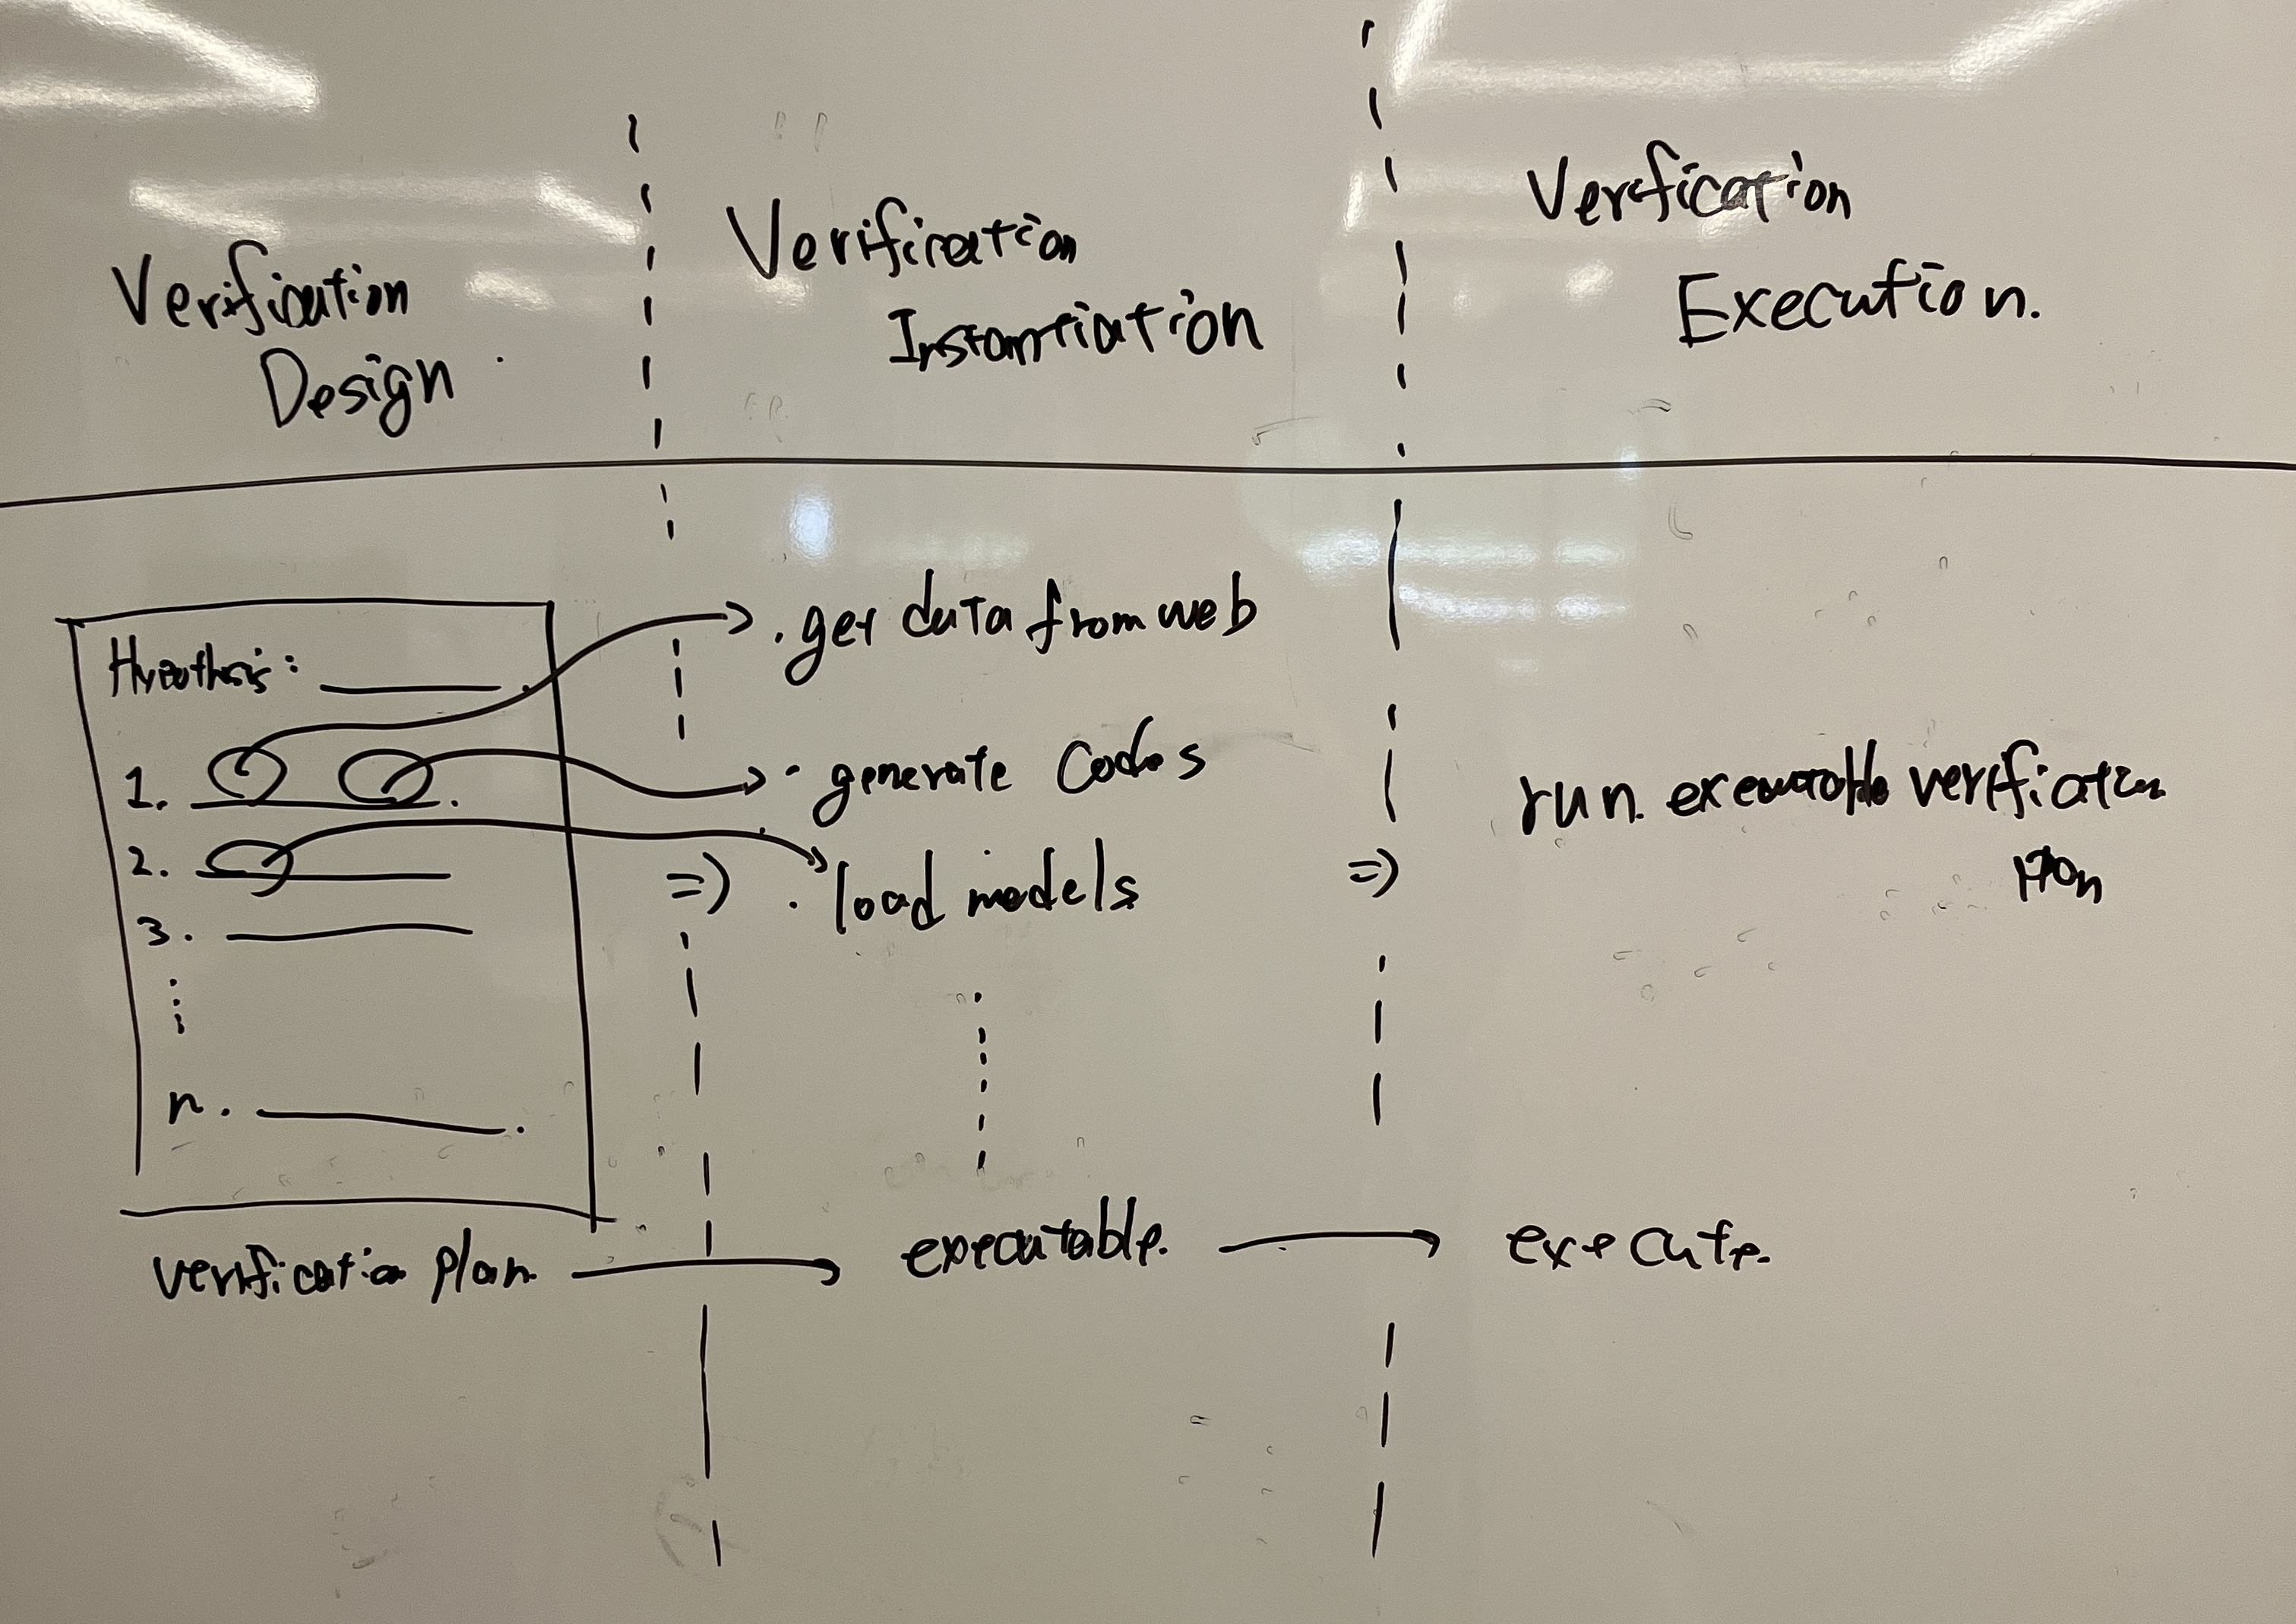
\includegraphics[width=\textwidth]{figs/verification.jpg}
    \caption{Verification}
    \label{fig:verification}
\end{figure}

\subsubsection{Verification Design} 
In verification design, the agent will create a plan to execute the verification, which consists of hypotheses, verification criteria (criteria to determine if the output confirms or refutes the hypotheses), and the procedures for conducting the verification. The verification plan should be specific and detailed enough so that anyone faithfully executing it can reproduce the same verification process and result. For example, suppose I am considering an experiment to compare a proposed method with a baseline and validate the hypothesis that the proposed method performs better. In this case, the plan should describe in detail which model to use, what dataset to employ, and how to measure the performance. Thanks to this specification, I can separates the two functionally distinct stages of verification: the phase of considering what needs to be validated and the phase of actually executing the verification.

It is during the verification design stage that specific skills for hypothesis verification are required. This is because automating the preparation and execution of a plan involves the automation of more general intellectual tasks, not limited to research automation, while creating a verification plan demands an explicit understanding of what verification entails and what criteria constitute a successful verification. In aiming to automate this verification plan, the key lies in teaching machines how to understand the concept of verification.\footnote{
Even humans may sometimes do verification without proper understanding of the method. For example, someone may conduct hypothesis testing just because ``everyone does it.'' While this may be an extreme example, it is not common for researchers to understand the epistemological implications of inductive reasoning and statistical inference and in what sense I can say I verify a hypothesis. In that sense, the requirement for machines to understand verification may be somewhat challenging. However, if the aim is to truly enable AI to autonomously conduct research, it appears crucial for the AI to have a proper understanding of what constitutes verification.
}

% Multiple abilities are needed to create a verification plan, but based on the discussion so far, it is evident that at least two abilities are required.


% At this stage, I contemplate how to validate the hypotheses and proceed to formulate a verification plan. In a verification plan, the agent writes about the hypotheses, verification criteria (what will be considered as evidence for verification), and the procedures for conducting the verification. These plans should be as much detailed as possible. The Fig. provides an example in the context of machine learning. The idea is to create a blueprint for a pipeline where verification is automatically executed by faithfully following the plan.

% Furthermore, for artificial intelligence to perform autonomous verification, it seems essential that the AI not only adopts certain verification criteria but also be able to explain the meaning behind them and how they contribute to the verification process. Even humans may sometimes engage in this without conscious awareness, such as conducting hypothesis testing because ``everyone does it.'' In that sense, this requirement may be somewhat challenging. However, if the aim is to truly enable AI to autonomously conduct research, it appears crucial for the AI to have a proper understanding of what constitutes verification and be able to design it itself or, at the very least, explain it adequately.

There are several abilities that a machine must possess in the context of verification planning, but based on the discussion so far, it is evident that at least two abilities are required: understanding what verification is and planning to achieve objectives.

Let's first discuss the ability to understand verification. As mentioned in the sections on question construction and hypothesis generation, this is an extremely crucial ability in the overall automation of the research process. As before, the extent to which ``understanding'' is required depends on how much autonomy is expected in the automation of verification. If that is used as a verification tool for humans, what machines to do is just using human verification methods properly. On the other hand, if they were required to understand the concept of verification from scratch, I would face a lot of challenges as I just described in this chapter. 

If you aim to achieve the former, one of the initial steps could be creating a dataset specifically tailored for verification. By gathering research papers that utilize widely used verification methods like statistical hypothesis testing, you can train a model to construct verification methods from these hypotheses. One naive approach could be to start by generating method descriptions in research papers from the given hypotheses. 

If you were to achieve the latter, you might want to begin by contemplating what beliefs mean for machines. Alternatively, placing agents in situations where verification becomes necessary could implicitly help them acquire the concept of verification. In this case, addressing the issue of generalization across environments, such as enabling machines to explicitly reuse the concept of verification, will be crucial. Eventually, as repeatedly emphasized, discussing how to resolve the alignment problem will be necessary.

% If artificial intelligence is used as a tool for human research, it is sufficient for artificial intelligence to faithfully reproduce what humans do as verification. For example, it would be great if it could use basic concepts such as hypothesis testing, controlled experiments, and interventions and automatically create experimental plans based on them. In this case, it is not necessary for the machine to strictly know why it constitutes verification, as long as it can learn from numerous examples of human verification and use it appropriately. In other words, in this case, the required understanding can be described as indirect and practical understanding through examples of human usage. Furthermore, if it can understand the concepts of hypothesis testing and controlled experiments from first principles, it would be a significant achievement in terms of automatic verification.

% On the other hand, if artificial intelligence itself is allowed to conduct research for its own knowledge generation, it seems that artificial intelligence needs to understand what verification is, whether explicitly or implicitly. And similar to the unknown nature of the answer to a problem, it seems to be an ability that cannot be acquired just by observing examples of human verification. This is because verification involves updating the beliefs of the members of a society, which depends on the nature of the beliefs of the machine group itself. Whether the knowledge generated by such agents is understandable by humans or can say something about nature is not obvious, but this will be discussed in detail in later chapters.

Let us move on the second ability: planning. Understanding verification is a necessary condition for setting verification criteria by considering what can be tested against a given hypothesis. When conducting actual verification, under the assumption of a hypothesis and verification criteria, one must devise procedures for carrying out the verification. For example, in experimental research, let's say a hypothesis A is formulated, and a verification criterion is established that considers the hypothesis valid if it meets certain criteria through statistical hypothesis testing. To actually perform this verification, it is necessary to generate data to be used for verification, and if there is no apparatus to generate the data, one may need to create it. Thus, in a verification plan, one must develop a plan to fulfill the purpose of executing the verification.

Creating a plan is known to be a challenging task, not limited to verification plans. To achieve a goal, one must understand what is necessary and comprehend the appropriate sequence of steps to achieve the goal. As mentioned earlier in the section on constructing questions, when creating a plan, it is essential to consider feasibility, taking into account the complex external factors such as current financial capabilities and accessible resources. Understanding and incorporating these constraints appropriately can be a highly challenging task, as they are intricately linked to various external factors.

While there are already a difficult task, the particular challenge in creating verification plans for research lies in the fact that one may need to create things necessary for verification if they do not already exist. This is an extremely high-level difficulty problem. To carry this out, one must first accurately identify what is currently lacking. After recognizing the deficiencies, one must consider how to create what does not exist. Once the method is known, materials for creating it must be prepared, and it must be actually built. And even if it is created, one must investigate whether they function properly. This is an unbelievably complex task, and it seems highly unlikely to simultaneously expect the creation of such intermediate products by directly generating a verification plan from the verification itself. Therefore, in aiming for true automation of verification, it is crucial to seriously consider how to solve this problem.


Finally, once the necessary elements for verification are understood, they need to be represented as something that can be understood by other researchers. This is not a requirement of a verification plan but a necessary condition for knowledge to become knowledge for society. In order to generate knowledge for society, it is necessary not only to verify hypotheses but also for the verification procedures to be understandable to other members of society and judged as valid.\footnote{
While it is desirable for the question generation process and hypothesis generation process to be publicly available, it is of utmost importance that the verification process is disclosed. 
} Also, as discussed in the section on hypothesis generation, verification must ensure that the causes behind the verification results are traceable as much as possible. While this is not an inherent requirement of the act of verification a hypothesis, it is a crucial characteristic needed for proper interpretation of verification results and for better knowledge production through hypothesis testing. As mentioned earlier, it is impossible to enumerate all potential assumptions, so it becomes necessary to explicitly state assumptions as comprehensively and in as much detail as possible to make the process realistic. Recognizing the underlying assumptions, including those behind the scenes, and selecting which assumptions to prioritize as potential causes of the results, is indeed a challenging task.



\subsubsection{Verification Instantiation} 
At this stage, the research plan that has been developed is translated into an executable instance. For example, if the research plan states, ``Train the model B with the dataset A...'' the necessary steps would involve acquiring dataset A from the appropriate source, formatting it to be compatible with the model's input requirements, and preparing the data for training, etc. Similarly, if the plan states, ``When a rat presses the switch B, food is dispensed...'' the agent has to prepare rats, food, and create a machine that dispenses food upon pressing the switch, and so on. This process involves translating the plan into physical or computational instance for execution.

\begin{figure}[htb]
    \centering
    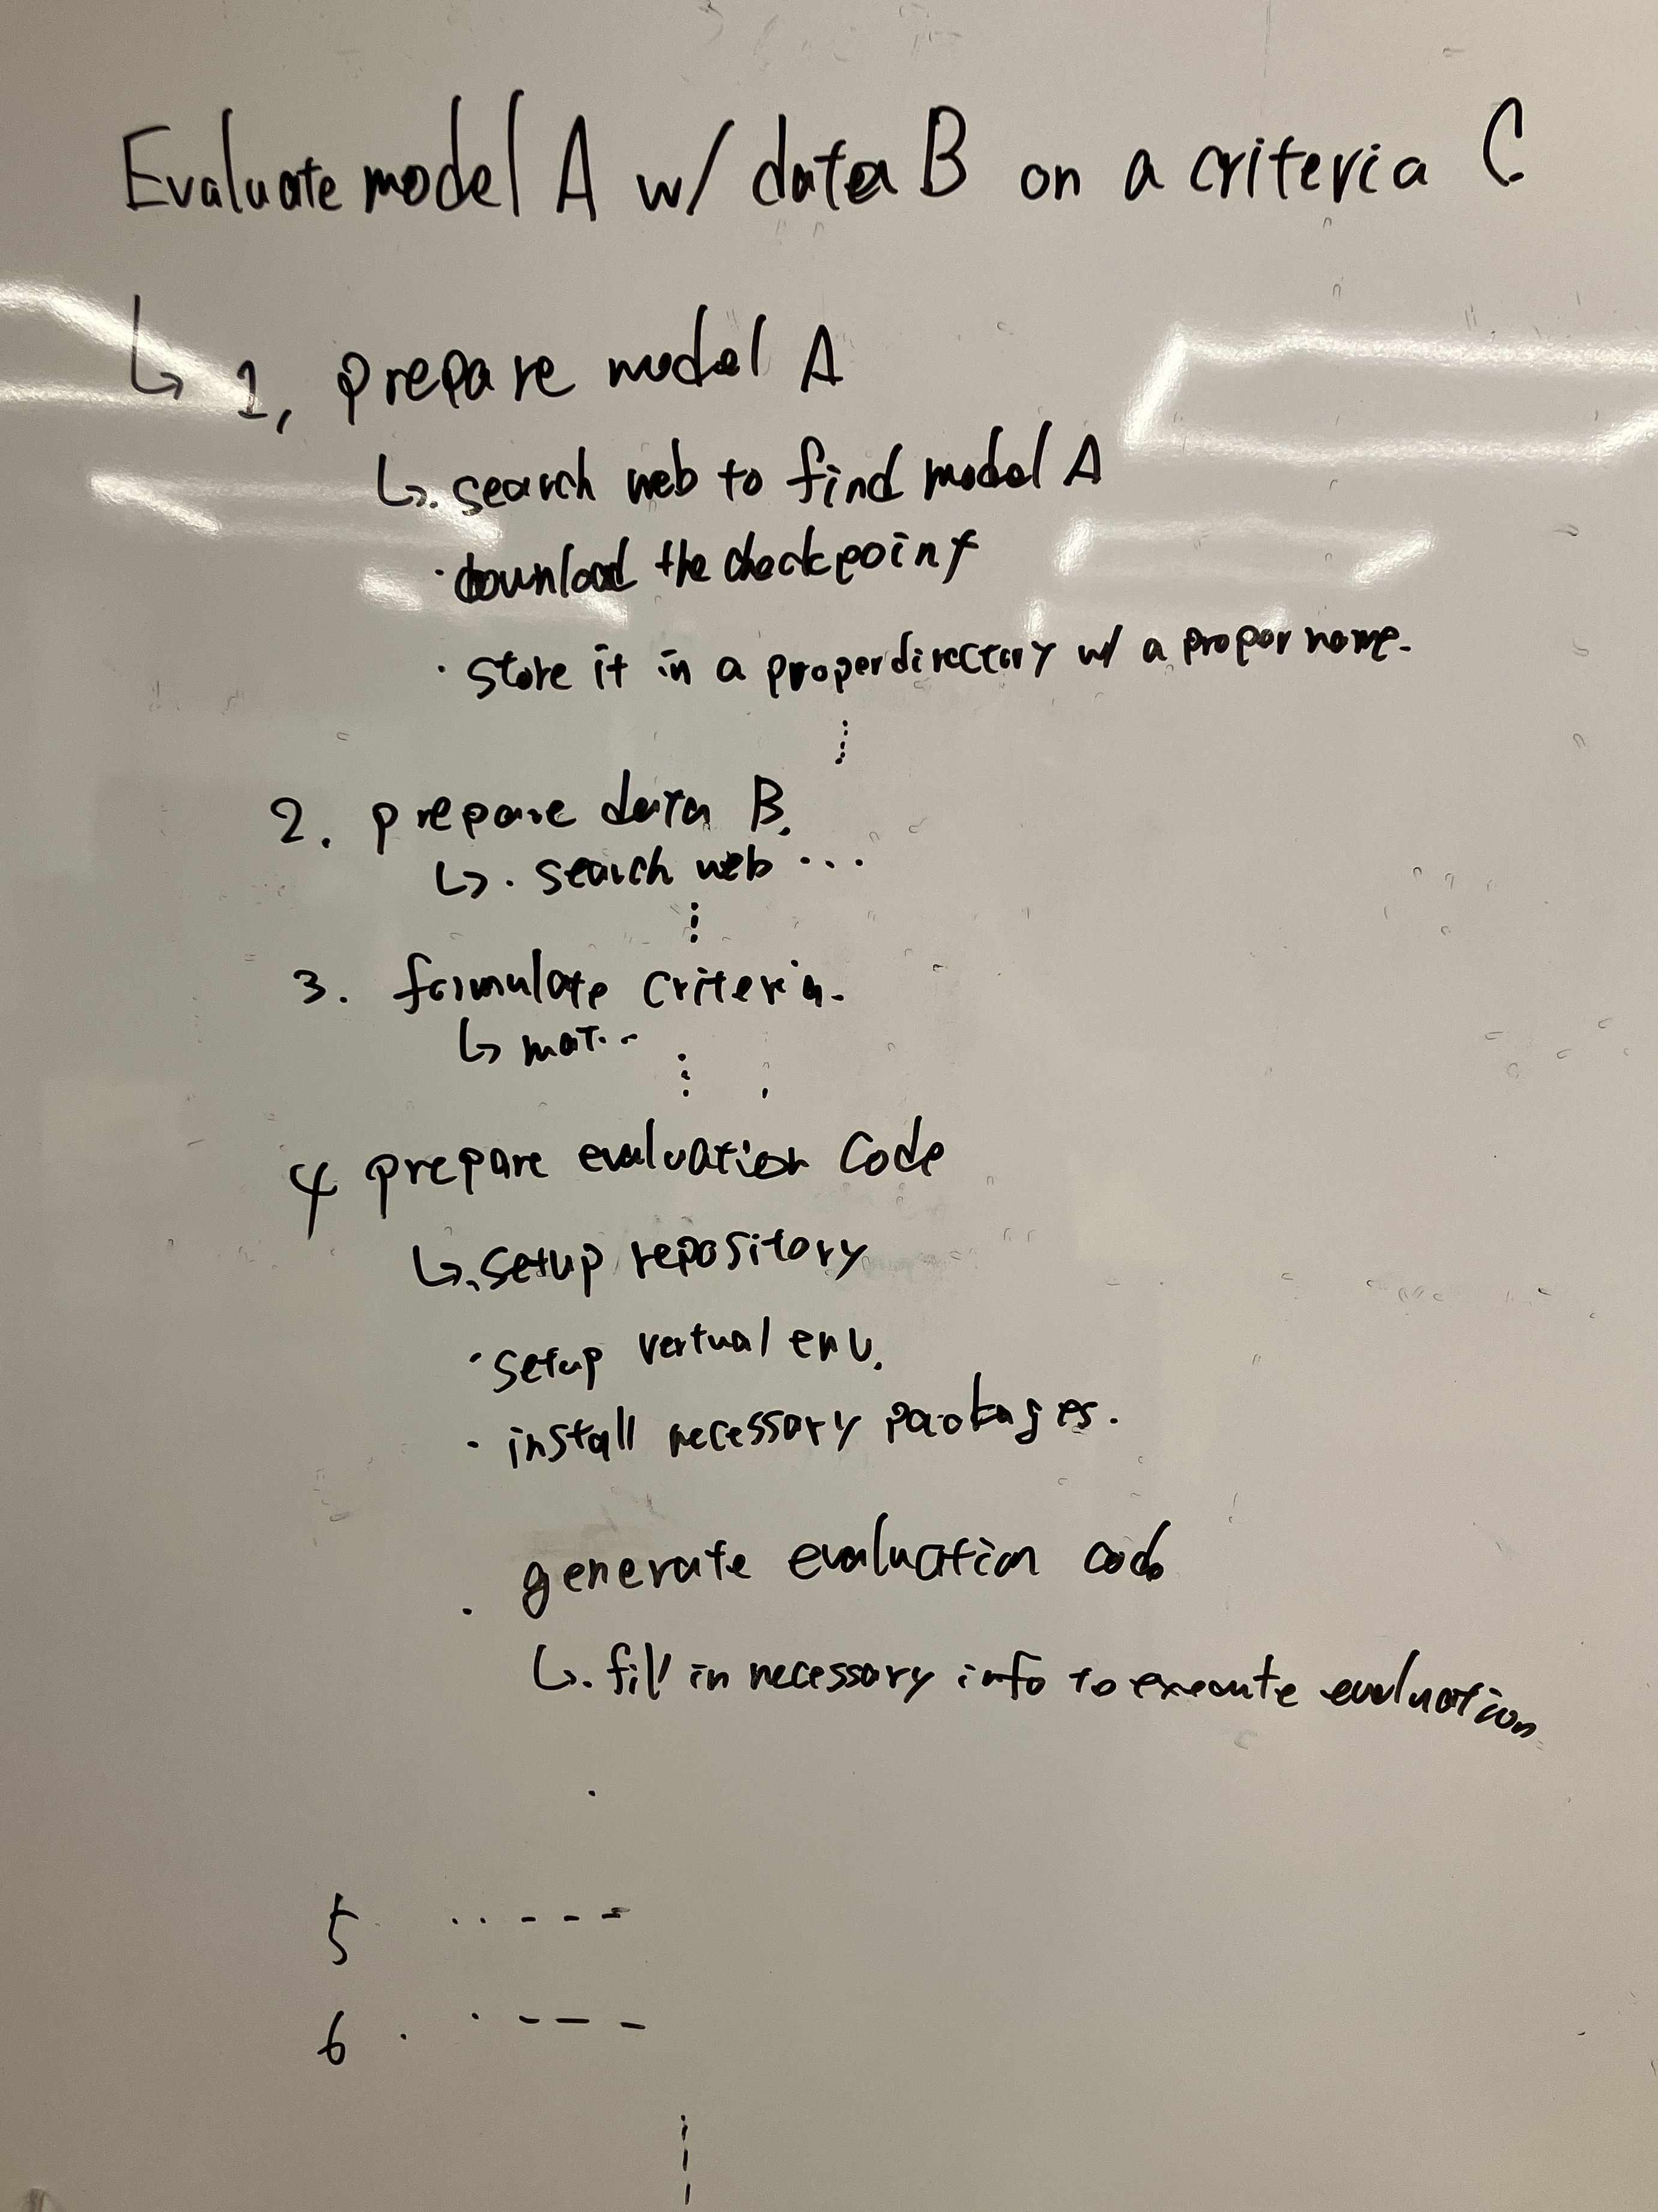
\includegraphics[width=0.5\textwidth]{figs/verification_instantiation.jpg}
    \caption{Verification Instantiation}
    \label{fig:verification_instantiation}
\end{figure}

As evident upon reading, this process is highly challenging to automate. Even research confined to the realm of computers, such as research of computer science, requires accomplishing a vast number of complex tasks. For research that necessitates physical realization in the real world, the development of robotics and embodied agents are necessary. Regarding the question of where and how to tackle these problems, I will provide my perspective in the later chapter. However, it is important to note that unless the research is constrained by questions and hypotheses, aiming for true automation will inevitably require overcoming these challenges

To reiterate, this process can be accomplished through the automation of actions, and it does not necessarily require unique technological developments for research automation. For instance, in studies that are entirely computer-based, automating all actions within the computer system would suffice. In recent times, attempts have been made to have language models operate computers, and the progress in such research corresponds to the advancement of automation in this process. If the research involves activities in the physical world, achieving full automation of human movements (or their equivalents) would make this process feasible. Therefore, research focused on developing humanoid robots that can move like humans will contribute to the automation of this process.

% Once a hypothesis has been established, a verification plan is created to determine how to verify it. The specific method of verification depends on the subject being investigated, making this aspect of research difficult to structurize and automate in a unified way.

% However, in many empirical sciences, the likelihood of a hypothesis is evaluated based on statistical significance. This is done by \textit{hypothesis testing} in practice. As this is a hypothesis test, it can only reject the null hypothesis, rather than directly determining the correctness of the hypothesis. Therefore, it can only be said that the hypothesis has survived for the time being. The belief that the surviving hypothesis is more likely to be valid is the basis for decision-making.

% In any case, humans seem to use statistics or probability as the basis for assessing the validity of a hypothesis. In other words, I seem to concede to consider a hypothesis as plausible if something that cannot happen by chance, such as observing the same number repeatedly. This is based on the assumption of the ``principle of confirmation,`` which assumes that if the number of observations increases, it can be considered more reliable, and the ``principle of uniformity,`` which assumes that things will continue to proceed as they have been if the conditions remain the saus. These beliefs ultimately serve as the basis for verification and scientific knowledge production. 

% I will not delve into the validity of these beliefs here. What matters is that my research activity follow a practice that ``when a hypothesis is present, and a certain criterion and procedure are prepared, and the hypothesis is considered valid according to that procedure, I consider it valid.''

% In theoretical research, sometimes there is no verification plan. Theory is a hypothesis, and its validity is determined separately through verification (not in the sense of whether it is mathematically valid, but for example whether it explains physical phenomena or not). However, in complex modern science, theorists propose a theory, and experimentalists verify it.

% Therefore, it is understood that in current research practice, shared knowledge in the form of papers may not necessarily provide a complete answer to a given question. This is similar to research on negative data. Negative data cannot solve the unknown initially declared, but it can reduce a certain degree of uncertainty towards it. This is because the validity of the presented hypothesis may have decreased somewhat. If this is the case, each research shared in the form of a paper may be more appropriate to describe as "reducing uncertainty towards the unknown," rather than "making the unknown known." This can become complicated when scrutinized strictly, so let's put this aside for now and continue to discuss how "producing new knowledge" is research.

% In reality, conducting research is expected to be done with limited resources (time, funding, computing resources, people, etc.). Therefore, it is necessary to consider these resources when determining the verification approach. After a research design is determined at an abstract level, the feasibility of the research plan is roughly evaluated through a simple problem setting. This is known as a pilot study.



\subsubsection{Verification Execution}
Finally, the instantiated research plan is executed according to the prescribed procedures. In verification design, I am crafting the essence of the verification, and during verification instantiation, I am preparing it to be executed in a concrete and feasible manner. Therefore, there are almost no tasks to be done in this process. The preparation for verification, being distinct from the actual execution of verification, is not a verification in itself. With this understanding, I have adopted this formal classification for the current context.
\footnote{
Typically,``experiments'' refers to the data generation process and subsequent analysis and interpretation are conducted separately. However, since I am discussing a verification plan in this context, all of them are in the same single plan. Therefore, please note that what emerges from executing the verification plan is not data but the verification results.

In many empirical studies, the data generated from experiments is often used not only for the verification of hypotheses but also for generating new hypotheses or giving some insights. However, as hypothesis generation and hypothesis verification play different roles in knowledge production, I do not assume any uses of the generated data beyond verification in this context. Of course, please note that this does not imply that such actions are prohibited in practice. Data analysis will be discussed in a separate section.
}

\subsubsection{Starting from Verification Design}

As mentioned above, I believe that the verification process can be divided into three stages: formulating a verification plan, preparing for the execution of the verification plan, and executing the verification plan. Among these stages, the execution of the verification plan and the preparation for it require interaction with the physical world in many fields. For example, in certain fields, you may need to purchase and raise rats for training, while in others, you may need to observe physical objects directly. On the other hand, formulating a verification plan is a process that is purely confined to the human mind in a wide range of fields. Therefore, it can be a good idea starting from automating verification design process.


\subsection{Verification Based on Statistics}
「正当化の根拠」とかにしておく?
人間は最終的に

Analyzing how statistical methods can validate hypotheses is crucial for automating hypothesis testing. Many research endeavors heavily rely on inductive inference to validate hypotheses, and statistics provide specific techniques for inductive reasoning. Therefore, I examine how I perform inductive inference using statistical methods, taking inspiration from Ohtsuka's arguments \cite{otsuka2022thinking}.

\subsubsection{Inductive Inference and Inference Statistics}

Inductive inference is a method of constructing general principles from data. We assume that data is sampled from a probability model and formulate the problem of inferring this probability model from the data as inferential statistics. The assumption of the existence of a probability model corresponds to the assumption of the uniformity of nature, which posits that similar situations will hold even in unobserved circumstances. As the uniformity of nature is a prerequisite for inductive inference, these formulations correspond to setting the foundation for inductive inference.

This probability model is assumed to be true as a prerequisite for inductive inference. However, in actual statistical inference, we perform inductive inference by establishing statistical models that approximate this probability model. In many cases, we assume specific families of distributions for these statistical models and reduce the problem to estimating parameters of these distribution families from the data. This is the formulation of inductive inference using statistical terms.

Within these formulations, the question arises of ``what kind of'' inductive inference we are performing. This precisely pertains to ``what is considered validated'' or ``how beliefs are justified.'' While multiple perspectives are possible, we will introduce discussions on classical hypothesis testing (referred to as just hypothesis testing below) and the approach using Bayesian statistics (referred to as just Bayesian statistics below).\footnote{
Note that this is not a discussion about what each position think about probability is, but rather a discussion on what they think is justification means.
}

\subsubsection{Bayesian Statistics and Epistemological Internalism}
In Bayesian statistics, we perform inductive inference by updating the degree of belief in a hypothesis based on the evidence provided by the data. The validity in inductive inference is adjusting the degree of belief in the conclusion in a consistent manner with the degree of belief in the premise. Representing the prior belief with prior probability and the likelihood with evidence, Bayesian statistics calculate the posterior probability following probability rules like Bayes' theorem. In this sense, Bayesian statistics, including Bayes' theorem, provides the logic for inductive inference. 

Ohtsuka argues that Bayesian statistics justifies beliefs based on a valid inference rule from other beliefs and compares this position to epistemological internalism \cite{otsuka2022thinking}.

\subsubsection{Classical Statistics and Epistemological Externalism}
In classical hypothesis testing, we first formulate some hypothesis regarding the probability model and then compare it with the data to either reject or retain the hypothesis. In other words, testing is a function that maps data to two options: rejecting or retaining the null hypothesis. Based on this result, we perform inductive inference (or behaviour). 

Ohtsuka interprets testing as a kind of examining tool that makes a judgment based on certain data and sees testing theory as a theory that measures the reliability of this examination tool. Making judgments about hypotheses based on data can be seen as a belief formation process, and testing theory educates the reliability of this process through measures like the size and power of the test. From this, classical statistical testing takes a stance that the justification of a belief is determined by the process through which it was formed, similar to epistemological externalism \cite{otsuka2022thinking}.

\subsubsection{For Automating Statistical Hypothesis Verification}

As such, when it comes to statistical methods for hypothesis verification, there are multiple perspectives on what constitutes justification. It is a challenging issue to known how various statistical techniques, each with their own approach, can provide evidence to substantiate a hypothesis based on the data \cite{otsuka2022thinking,sober2008evidence,sep-statistics}. When seeking to allow machines to autonomously conduct hypothesis verification, determining what they should be capable of is a challenging issue. 

\subsection{Challenges for Automating Hypothesis Verification}

\subsubsection{The Inherent Difficulty of the Act of Verification}
In the first place, the act of verification is a highly challenging process. Firstly, as mentioned earlier, inductive approaches cannot verify hypotheses in the same way as deductive reasoning. Also, I notice that hypothetico-deductive method, which involves verifying claims derived from a hypothesis to confirm its validity, is still widely used today. However, verifying a deduced claim does not support the hypothesis because there may be many hypothesis that can result in the same deduced claim. In response to these, Karl Popper proposed that while hypotheses cannot be confirmed, they can be falsified \cite{sep-scientific-method}. However, in practice, the verification of hypotheses involves implicitly relying on numerous auxiliary hypotheses. When using experimental apparatus, it requires many assumptions to trust them. Even when an experiment fails, determining whether the hypothesis was incorrect or the experiment itself was flawed is not as straightforward as one might think. Thus, there is inherent uncertainty in attributing the results of verification to a specific cause \cite{chalmers2013thing,sep-physics-experiment,sep-scientific-underdetermination} as I have discussed in the section of hypothesis generation. Furthermore, all reasoning and observational evidence are inevitably influenced by some form of theories, individuals, or societal factors \cite{sep-science-theory-observation}. Therefore, it is necessary to carefully examine them to ensure that they are not distorted by unintended influences. 

\subsubsection{The Difficulty of General Hypothesis Verification}
I recognize that the the way to verify a hypothesis is strikingly diverse, as it can significantly differ depending on the subject of research. For instance, if one wishes to study the behavior of rat, they may need to train the rat. On the other hand, if you want to test a theory of particle physics, you may have to construct and run a huge particle accelerator. In the field of history, the existence of historical records might serve as evidence, while in mathematics, the verification process revolves around the proofs themselves. Due to this high degree of flexibility, hypothesis verification can be the most challenging aspect to automate for realizing a ``general'' artificial researcher.

% \subsection{How to Justify Beliefs}
% In many empirical sciences, statistical methods occupy a privileged position as the primary means of verifying hypotheses. Therefore, it seems important to consider in what sense I can say that a statistical method can validate hypotheses, while I admit that the methods of verification vary greatly depending on the type of question or hypothesis and it cannot be said that there is any universal method for verification. The use of inferential statistics methods is widely accepted, but it is a challenging issue to known how various statistical techniques, each with their own approach, can provide evidence to substantiate a hypothesis based on the data in the real world \cite{otsuka2022thinking,sober2008evidence,sep-statistics}. Thus, what constitutes the verification of a hypothesis, or in other words, the justification of a belief, is a very difficult debate in which it is likely challenging to arrive at a unified answer. Please note that the discussions mentioned earlier, such as the uniformity of nature, pertain to the validity of induction itself. In statistical methods, however, induction is assumed and the discussion begins with formulating this uniformity by assuming a probability model. 

Furthermore, as explained in the section on statistical hypothesis testing, it was also described how even with inductive inference using the same statistical theory, there are multiple perspectives on how it justifies beliefs. Even empirical sciences, which employ highly universal verification methods based on statistical approaches, face such difficulties. Therefore, aiming for autonomous acquisition of verification methods in broader fields of research would likely pose even greater challenges. These issues will require further in-depth discussions in the future.

% This discussion of statistical method provides important insights for the pursuit of developing AI capable of conducting autonomous research. As can be seen from the assumption of being rooted in machine learning, the validity of inductive inference itself is generally accepted and not a practical concern in creating such AI. However, how to make agents acquire the methods of justification is a important issue. If the criterion for justifying beliefs is to be acquired completely autonomously from scratch, it may very well lead to criteria that are meaningless for humans. Additionally, it seems that the criteria for justification employed by humans are diverse. When properly considering the reasons that these criteria are believed to provide justification, I can recognize that there are highly intricate structures involved. In light of such considerations, the extent to which one can understand and acquire criteria for justification from the criteria humans already employ is a nontrivial problem. 


% I do not intend to claim that these uncertainties undermine the reliability of research. Such uncertainties exist in almost all human endeavors. Research, among these activities, strives to confront these uncertainties with great care and rigor. Above all, the fact that the results generated through research have effectively supported my lives demonstrates their efficacy.

% I mentioned the difficulties inherent in verification to highlight their significance, particularly when considering autonomous artificial intelligence capable of self-verification. Ideally, autonomous agents are expected to establish their own methods and criteria for verification. However, if verification inherently carries such difficulties and uncertainties, the more rigorously I consider it, the more paralyzed the agent becomes, as it seemingly cannot accomplish anything. \textcolor{red}{TODO: Add explanation}

% A characteristics of research can be found in the systematicity, rigor, and objectivity of research practice \cite{sep-scientific-method,hoyningen2008systematicity,haack2003defending}. 

% In particular, I believe that a characteristic of research lies not in the way of determining questions or generating hypotheses, but in the fact that the verification of hypotheses is done in an extremely rigorous and careful manner. 

% It could be said that I'm taking a view similar to the new experimentalism, placing emphasis on verification in research, or experiments \cite{chalmers2013thing,mayo1996error}.

% Of course, generating a hypothesis is not a simple task. What I want to say is that, as long as any method of hypothesis generation is properly verified, it is considered research, and no matter how properly a hypothesis is proposed, if the verification is sloppy, it is not considered research. This means that verification may be at the heart of knowledge production. In other words, in order to create artificial intelligence that produces knowledge, it is important to consider how to create an intelligence that can perform verification.

\subsection{Autonomous Hypothesis Verification}

\begin{figure}[htb]
    \centering
    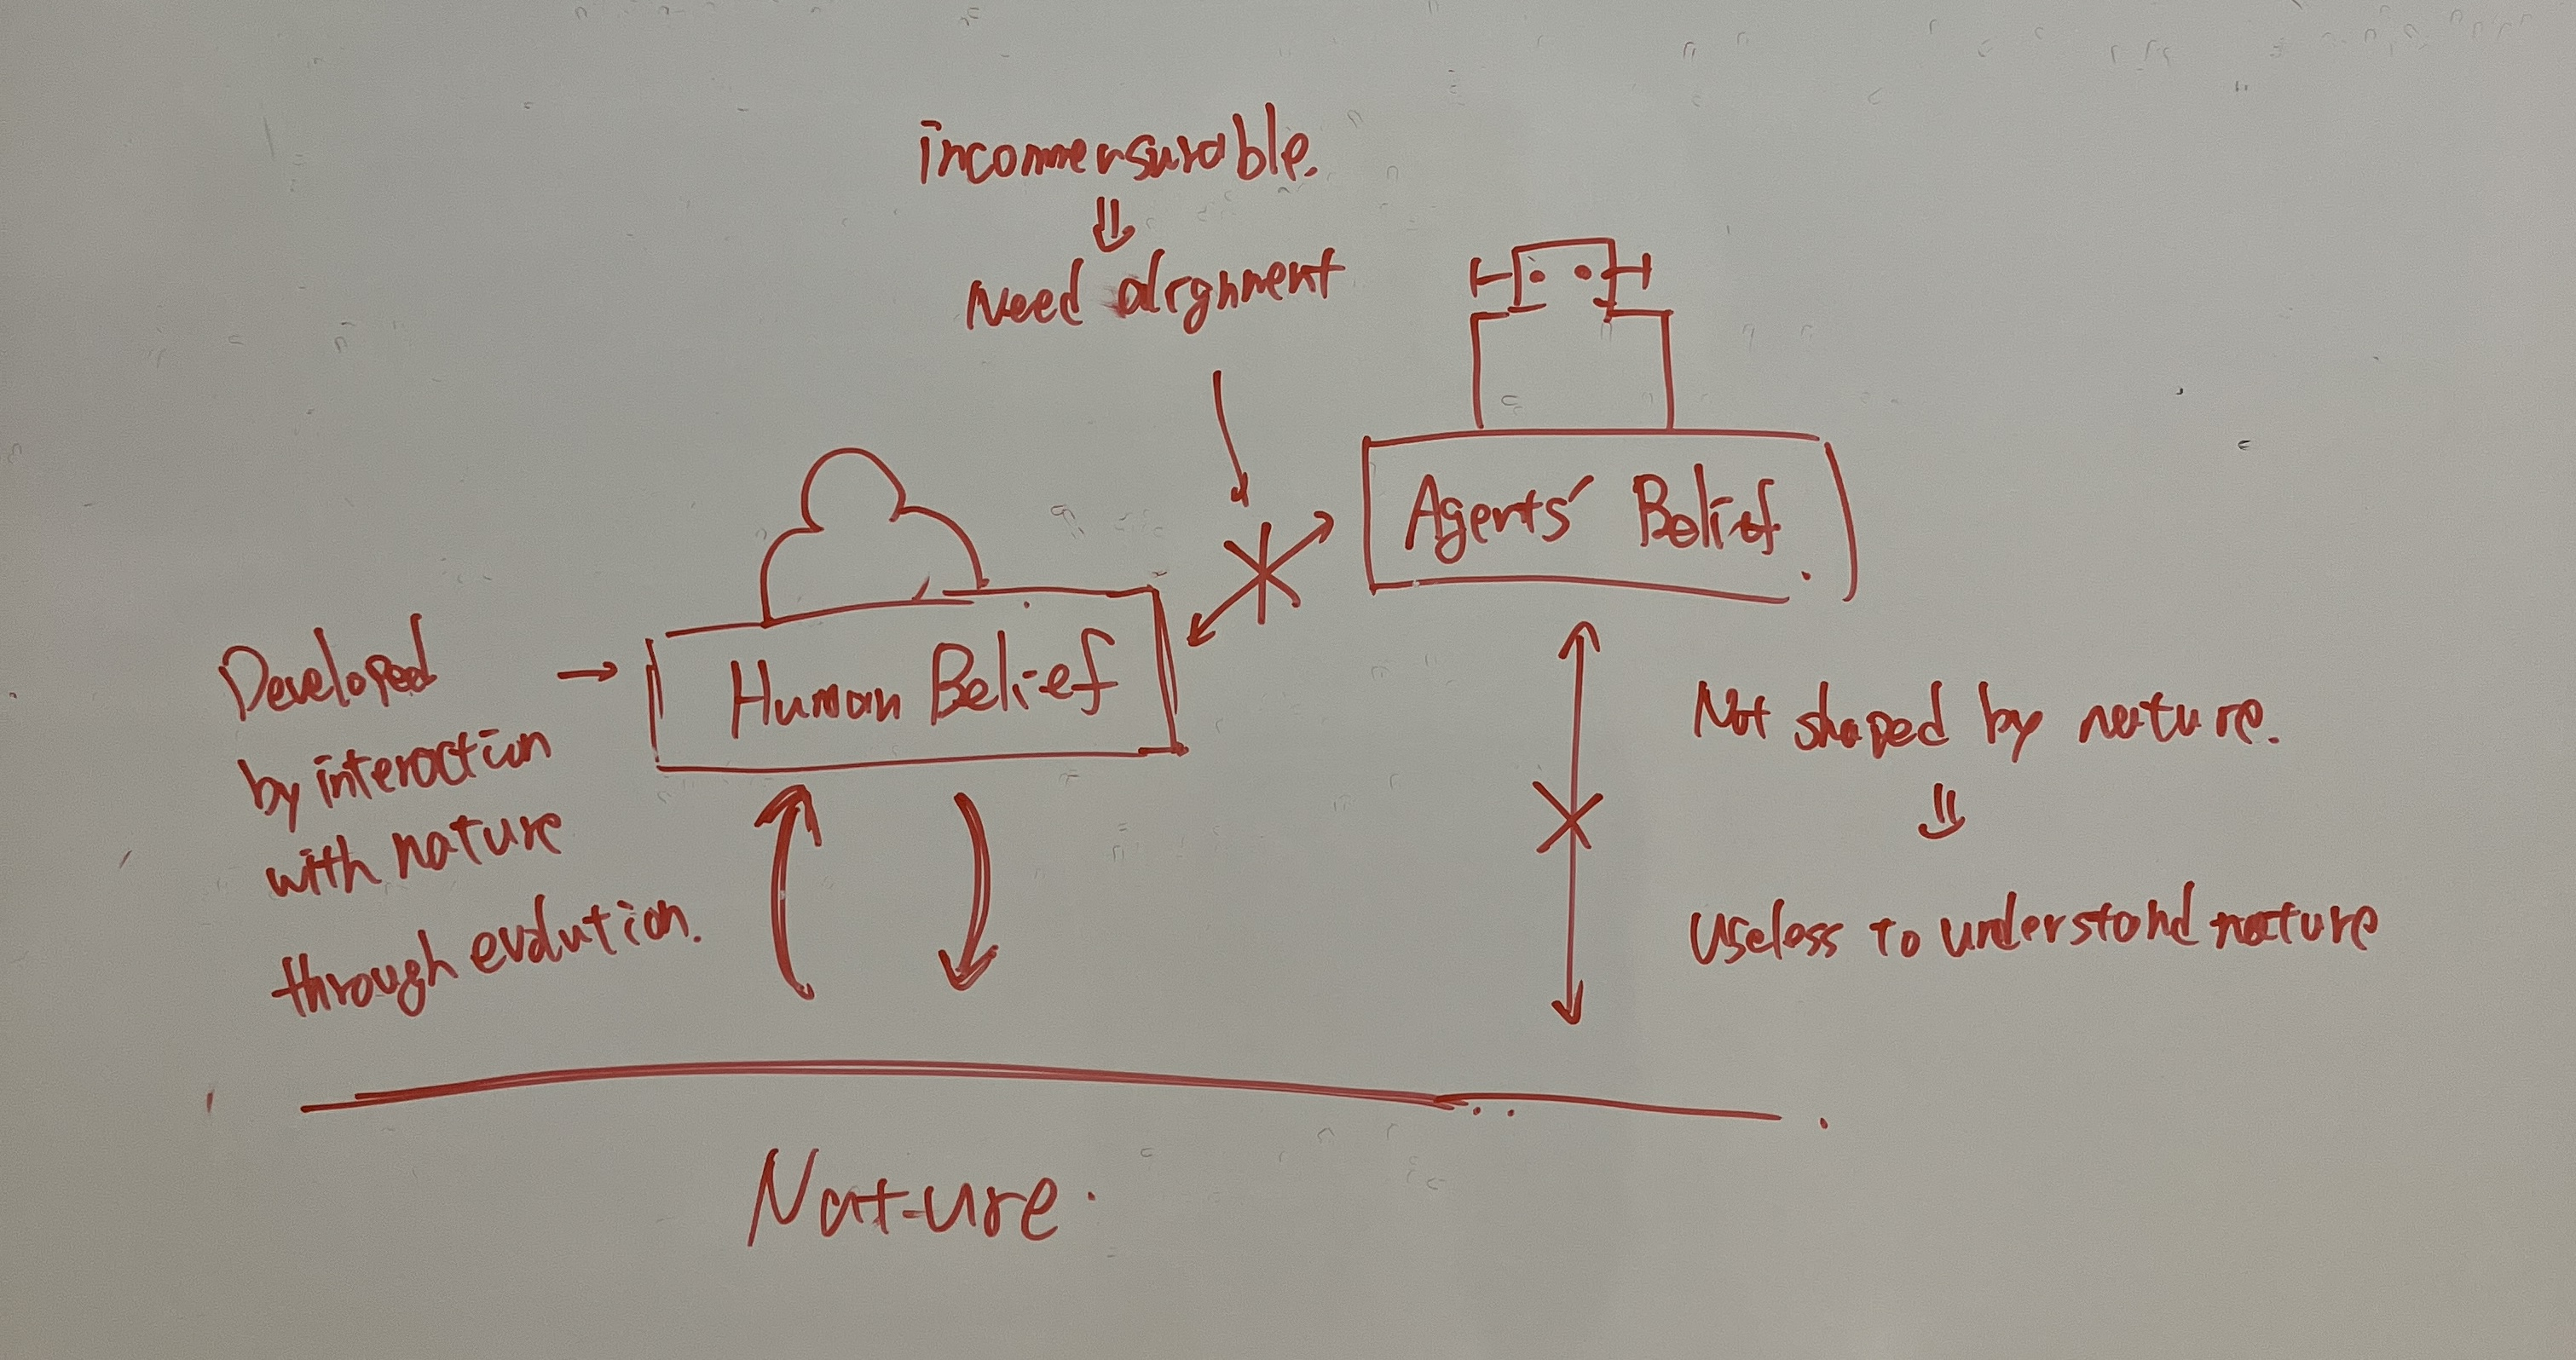
\includegraphics[width=\linewidth]{figs/incommensurability.jpg}
    \caption{Incommensurability}
    \label{fig:incommensurability}
\end{figure}

I said that research is to generate knowledge for humanity. However, this is merely because humans have been the only ones conducting research thus far. I believe that in principle there could be knowledge for beings other than humans and hence research for them as well. 

For example, if a group of machines are each capable of holding certain belief state which is similar to each other, they seem to be able to hold a shared belief. If these agents have a way to ground their belief that a hypothesis is true to their shared belief, then this can be regarded as research within that society. Therefore, the definition of knowledge as belief leads to the conclusion that research by and for the machines would look like this.

\begin{figure}[htb]
    \centering
    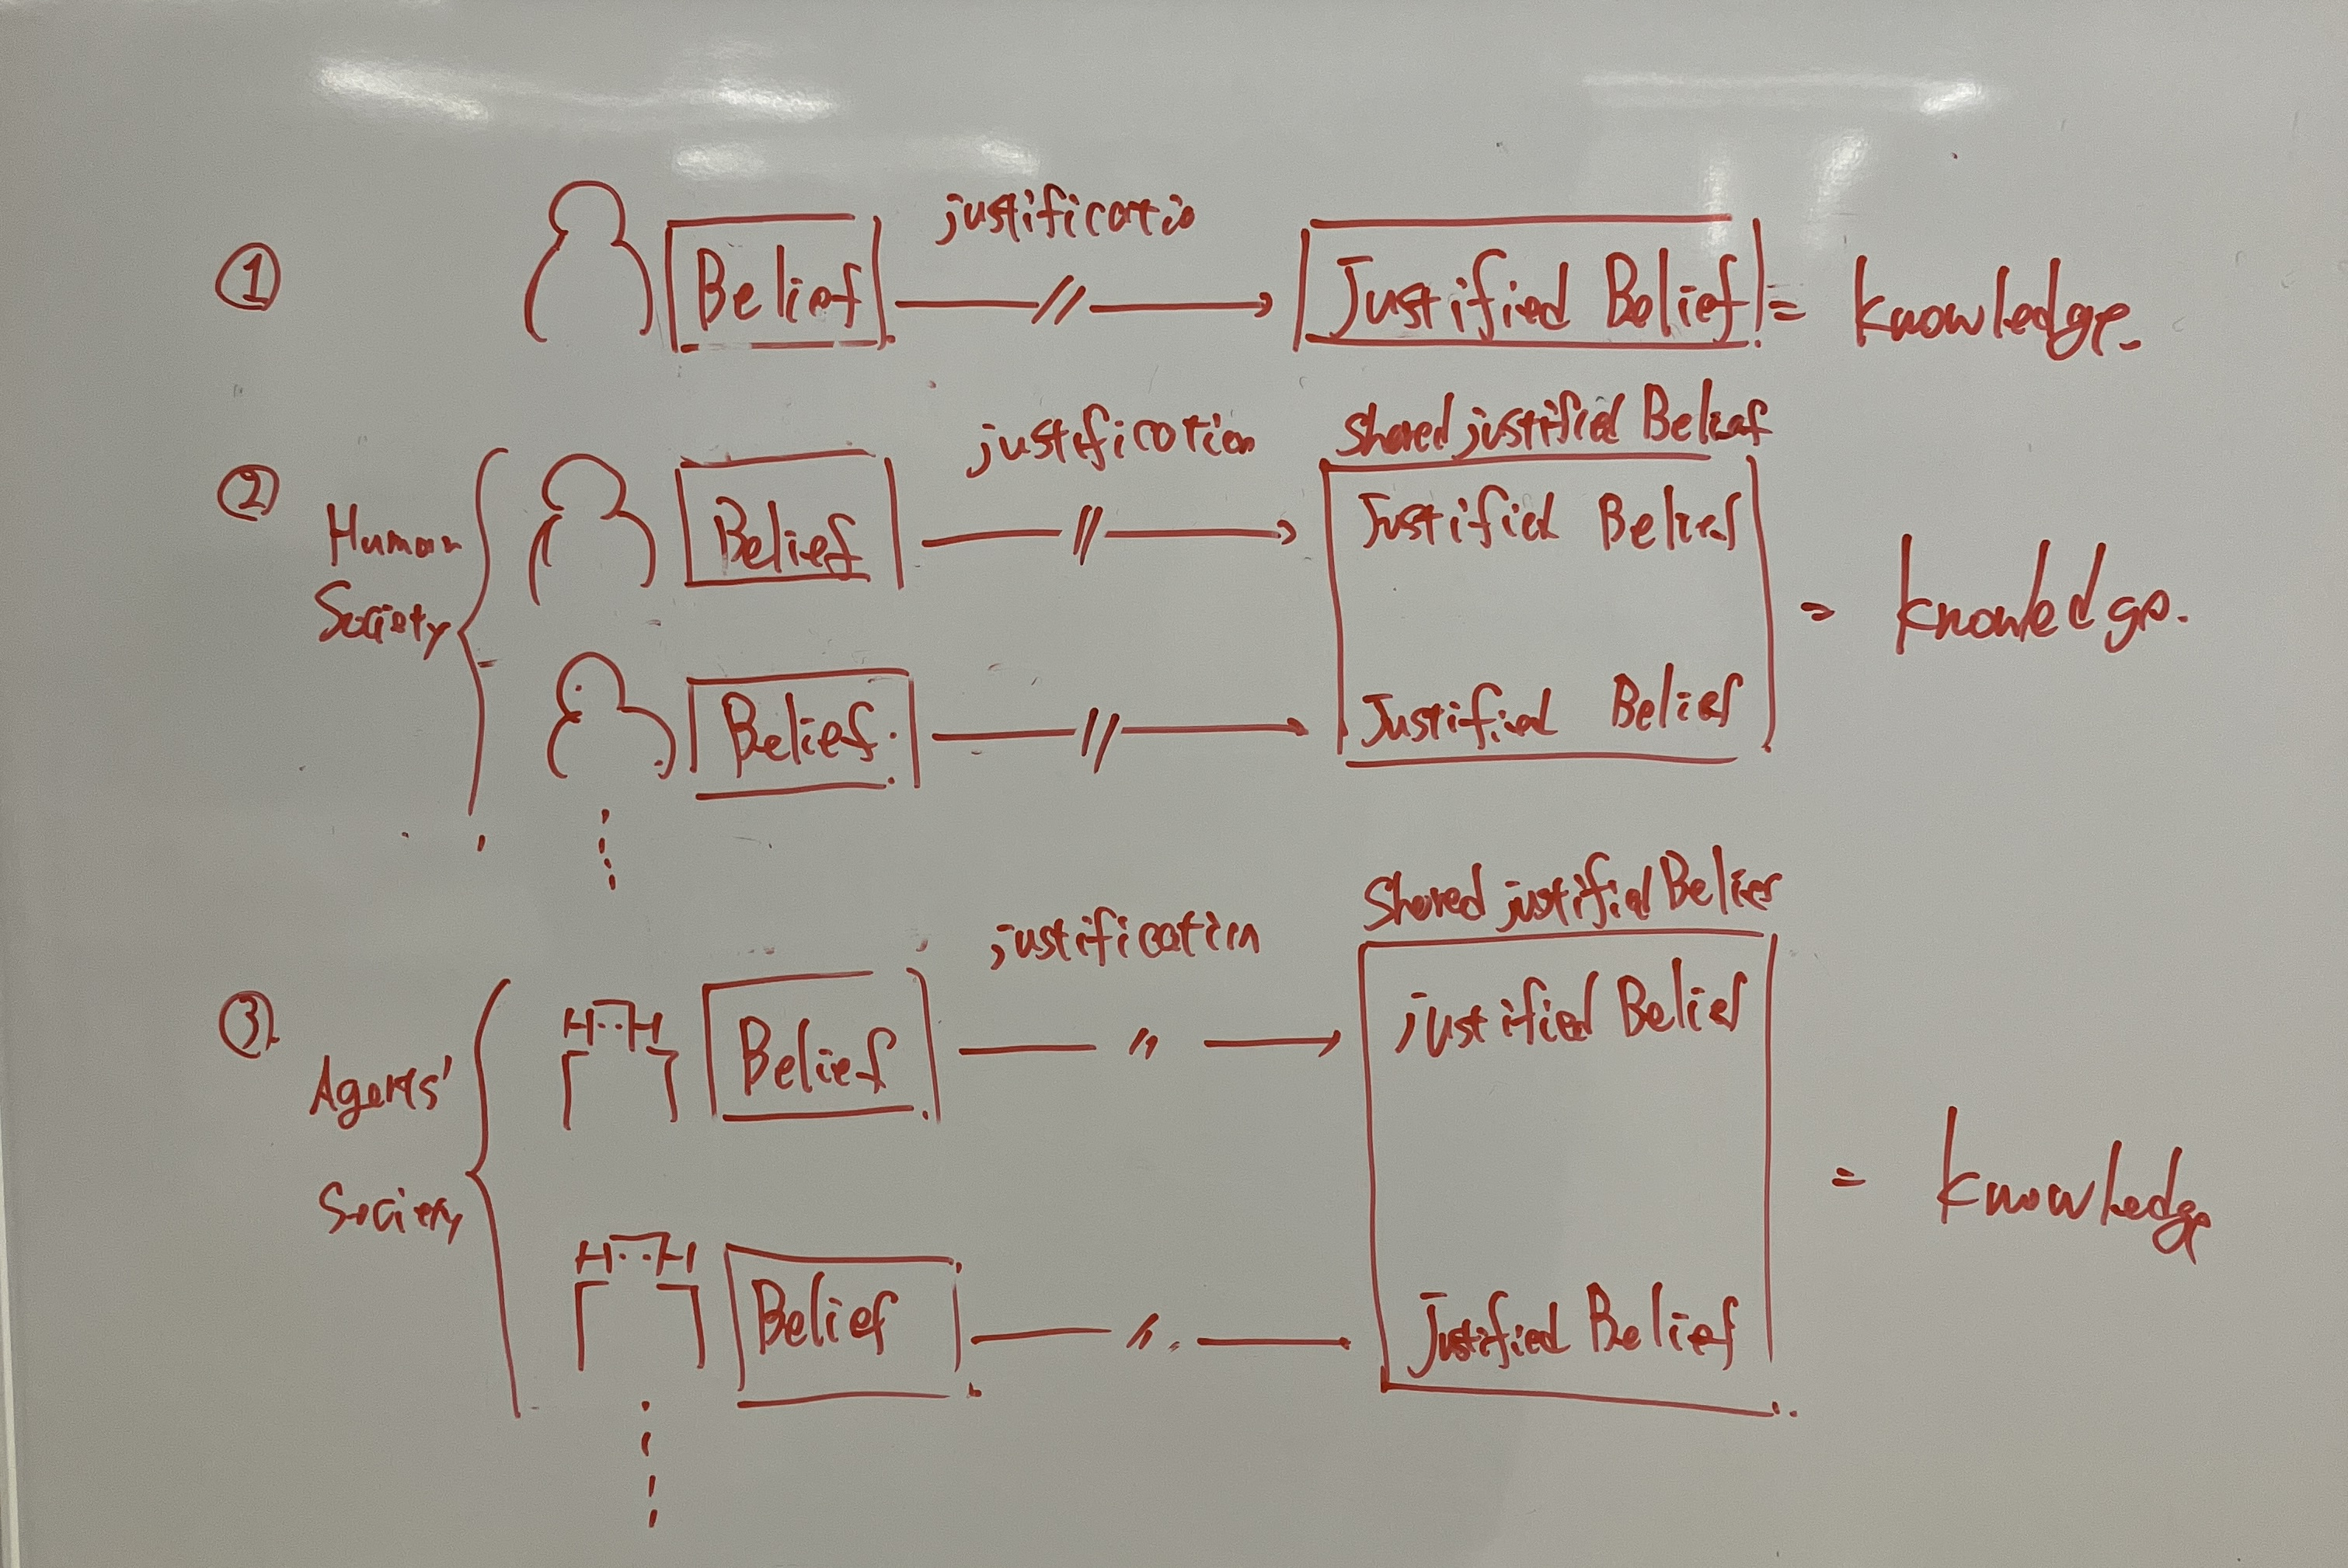
\includegraphics[width=\linewidth]{figs/shared_belief_revision.jpg}
    \caption{Belief Revision}
    \label{fig:shared_belief_revision}
\end{figure}

There are two implications here. Firstly, if we let AI entirely autonomously conduct research in the sense of current definition, including the design of the conceptual foundation of verification, they would likely produce nonsense for humans. This is because the systems of beliefs of humans and those machines would be entirely different from each other. Therefore, to conduct research that is meaningful to humans, it could be said that the foundation of the method of verification should be based on the foundation of human verification.

The second implication is that if the foundation of verification is autonomously constructed, the AI capable of conducting research in the sense of this definition would even produce knowledge meaningless for understanding nature. This is because while human beliefs have been shaped to be consistent with nature through interactions with it, the beliefs of machines are not necessarily so. Through the process of evolution, humans have spent vast amounts of time interacting with and modifying their bodies to survive in nature. Our beliefs are formed in such contexts, and the beliefs we currently possess are likely advantageous for living in nature. Therefore, I believe that our strong belief serves as a reliable foundation for understanding nature. Machines do not possess bodies embedded with such interactions with nature. Therefore, just because they have strong convictions does not guarantee that these will serve as a reliable foundation for explaining nature. 

When aiming for artificial intelligence that can conduct research autonomously, we still do not know how much can be entrusted to AI, namely, where the limits of autonomy lie. Based on the above two conclusions, it becomes apparent that when letting AI conduct research in the current definition's sense, it seems difficult to have AI create the conceptual foundation of verification from scratch. Therefore, it appears necessary to teach this AI what verification entails through human examples or align their values regarding verification with human values.

\chapter{Landscape of Research Fields for Research Automation}
\label{chapter-literature-review}

% 本章では、研究の自動化を目指す試みを幅広く紹介します。特に、これまで同じ論文上やコミュニティ間で論じられることがなかった研究たちも含めて、「研究の自動化を目指す研究群」として統一的に紹介しようと思います。一つ一つの論文を丁寧に紹介することは現実的ではないため、あくまで本論文では各分野や研究の取り組み全体をごく簡単に紹介することに注力します。各分野での研究成果についての詳細な説明については、すでにいくつもの素晴らしいレビュー論文が出版されていますので、そちらをご参照ください。ただし、近年の言語モデルを用いた取り組みについては個別の事例も扱いながら紹介しようと思います。

% 各分野を紹介した後で、汎用的で自律的な人工研究者という観点から、それらを分類する二つの軸を提案します。一つ目が汎用性の軸で、これは各研究の自動化の取り組みが、どれぐらい広い研究領域に対して汎用的なタスクを自動化するものであるかというものです。例えば、科学研究全てで必要となるようなタスクの自動化はある特定の研究課題を自動化するようなものよりも汎用的であると言えます。二つ目が研究過程のどの部分を自動化しているか、という軸です、これは自律性の軸に対応します。例えば、ある研究は仮説生成全体を自動化しているかもしれませんし、別の研究は仮説検証の特定の過程のみを自動化しているかもしれません。全ての研究過程の作業が自動化されている場合、これは自律性が高いと言えます。

% 最後に、研究分野の紹介と軸の提案を踏まえて、研究の自動化に関するパースペクティブ論文・レビュー論文のうちいくつかについて論じます。特に、紹介されている個別の研究よりも、それらの研究がどのようにして既存研究を整理しているか、どのような提案をしているかを見ていきます。これによって、本論文による整理の位置付けを改めて明確にし、次章以降の議論に繋げていきます。

\section{Existing Discussion on Research Automation}

Attempts to automate research began soon after the advent of computers. Until then, humans had developed science by describing experiences (primary science) and by making predictions through the construction of theories (secondary science). With the advent of computers came simulation science (third science), which uses computers to automate complex scientific computations, and data-driven science (fourth science), which automates the discovery of laws from large-scale data \cite{hey2009fourth}. Within the individual academic discipline ``X,'' the third science gave rise to the field of \textit{Computational-X} and the fourth science gave rise to the field of \textit{X-infomatics}, leading to the automation of entire academic disciplines.

\subsubsection{AI for Science}

Automation of scientific research with AI, including logical AI, has been an area of interest since the advent of AI \cite{langley1987scientific}. In the early stages of research, researchers created logic AIs that mimics the problem-solving process of researchers \cite{lindsay1993dendral}.

The remarkable performance of deep neural networks has now made almost all scientific fields more or less influenced by AI. The term \textit{AI for Science}, which automates scientific research with machine learning, has appeared due to the remarkable development of machine learning technology since the 2010s. 

AI for Science is a concept that encompasses a very wide range of initiatives. All attempts to solve problems in any process within science using machine learning or to develop the foundational technologies for them can be considered within the scope of AI for Science. Indeed, a vast number of machine learning application studies have been generated in numerous scientific fields \cite{xu2021artificial}, such as AI for Material Science and AI for Medical Science, named few.
\footnote{In this paper, it is not possible to introduce each of these individually, so we will omit the introduction of application studies in each research area of AI here. There are several excellent review papers available, so if you are interested, please refer to those.}

Wang et al. \cite{wang2023scientific} have excellently summarized these activities, we will introduce existing automation efforts while borrowing the view of their work. They categorize and organize various initiatives in AI for Science by focusing on which scientific processes they are related to: data handling, hypothesis generation, and simulation and experimentation \cite{wang2023scientific}. This is based on the view that the essence of science lies in the collection, transformation, and understanding of data.

The group of studies that incorporate biases to handle scientific data on AI, giving it information about the governing physical rule, is called \textit{physics-informed machine learning} \cite{karniadakis2021physics}. The incorporated biases include the ability to handle partial differential equations (PDE), symmetry, and intuitive physics \cite{hao2022physics}. Karniadakis et al. \cite{karniadakis2021physics} and Hao et al. \cite{hao2022physics} systematically and clearly summarize existing research from the perspective of which elements of machine learning are modulated by which biases and how they are incorporated. % TODO

The ability to handle PDEs gives us the basis for both the simulation of physical models and the discovery of the law from data, which we will discuss later. Studies that aim for better inductive biases and architectures in deep learning by treating symmetry as a first principle are called \textit{geometric deep learning} \cite{bronstein2021geometric}. Given the importance of symmetry in natural sciences, this group of research also plays a significant role in AI for Science. Zhang et al.  organize existing research in AI for Science across different research domains, focusing on symmetry as one of the common foundational pillars \cite{zhang2023artificial}.

The methods for generating hypotheses vary significantly depending on the subject, so there exists a wide range of approaches to automate this process. For example, attempts to generate hypotheses from articles or from scientific data are being undertaken in all research fields. 

One long-standing approach to hypothesis generation by AI is the research focused on discovering symbolic equations that describe scientific laws from data (\textit{equation discovery}). Among the earliest pioneering studies in this area, the BACON system by Langley et al. \cite{langley1987scientific}, and subsequent studies based on it, are well-known. In particular, the research on equation discovery that is mainly studied in the machine learning community is known as \textit{symbolic regression}, which originally started from research that used genetic programming approaches to discover symbolic equations.
 Kramer provides a comprehensive overview of the history of equation discovery research, including early studies that did not utilize machine learning \cite{kramer2023automated}. Famous deep learning approaches include AI Feynman \cite{udrescu2020ai,udrescu2020ai2}, which transformed the problem itself into a simple form and discovered the fundamental physical laws selected from Feynman's physics lectures.

% Symbolic regression is a problem of exploring a combinatorial hypothesis space among hypothesis generation \cite{wang2023scientific}. 
In science, exploration plays a crucial role, as exemplified by the search for hypothesis spaces and experimental conditions mentioned later. Therefore, methodologies for better automated exploration by machines have been sought, using techniques such as active learning. There is a perspective paper of research automation by Kitano \cite{kitano2021nobel} that focuses on the importance of machine-driven exploration of hypothesis spaces. Kitano points out that current hypothesis selection is value-driven, based on human value criteria, and argues that we should aim for hypothesis generation through exhaustive machine-driven exploration that is not dependent on such human value criteria. He points out that some of the Nobel Prize-winning research is actually the result of such exhaustive exploration, emphasizing the importance of this approach.
% \subsubsection{Symbolic Regression / Equation Discovery}
% % \subsubsection{Symbolic Regression} 
% Scientists have constructed models in the form of mathematical equations that explain them from observational data. This has enabled us to go beyond observational data to understand and predict underlying phenomena. That is to say, formulating a mathematical representation that elucidates the phenomenon behind the data is an extremely critical step in science. 

% One attempt to automate this endeavor is \textit{symbolic regression} \cite{makke2022interpretable}, or \textit{equation discovery}. These are attempts to infer from the data a formula that explains it. While classical approaches to symbolic regression have traditionally employed methods such as evolutionary computation, recent years have seen the emergence of strategies utilizing deep neural networks \cite{petersen2019deep,udrescu2020ai,udrescu2020ai2,cranmer2020discovering,kamienny2022end,d2022deep}. Some researchers have proposed the frameworks \cite{landajuela2022unified,keren2023computational} and benchmarks \cite{matsubara2022rethinking} for symbolic regression. You can find a literature review of symbolic regression in \cite{makke2022interpretable}, and that of the early studies in \cite{kramer2023automated}.

Once a hypothesis is formed, it is tested through experimentation. An experiment is the act of generating observational data through a set of predefined procedures. In modern science, simulations are used to generate data that resembles observational data. To create better simulations, knowledge of scientific computing is essential. The attempt to automate the generation and analysis of scientific data by combining scientific computing and machine learning is known as \textit{Scientific Machine Learning (SciML)} \cite{baker2019basic}. In physical simulations, numerical solutions to differential equations often come into play, so physics-Informed Machine Learning is also frequently discussed in this context. Experiments and numerical calculations come with uncertainties, so there is a long history of research on quantifying these uncertainties (\textit{uncertainty quantification}). This is also an important topic of study in SciML.

There is also a long history of research applying machine learning to experimental design. In particular, research on the efficient search for experimental conditions using active learning, including Bayesian optimization (\textit{Bayesian experimental design}), has been attempted in various application fields.

% 特に科学技術計算と機械学習を組み合わせて科学データの解析を自動化する試みは Scientific Machine Learning (SciML) と呼ばれています。(シミュレーション)

% 機械学習において科学データを扱えるような帰納的バイアスを組み込む研究群は Physics-informed machine learning と呼ばれています。組み込まれるものとしては、直観物理、微分方程式を扱う能力、対称性を抽出する能力などがあります。微分方程式の取り扱いは科学計算がずっと扱ってきたものですので、微分方程式を扱う研究は SciML の文脈で議論されることも多いです。また、対称性は幾何学的構造の保存なので、これらは geometric machine learning の一つとして議論されています。

% データからそのデータの背後の法則を記述するシンボリックな方程式を推定する試みも行われてきた。機械学習を用いてデータから方程式を推論する、symbolic regression がある。方程式を発見するシステムの先駆けとして BACON がある。2000年代には単位による制約から数学的に可能な方程式を同定する研究も行われた。これらは equation discovery という名前で研究されてきました。

\subsubsection{Workflows for Automation}
Some studies have attempted to represent scientific research pipelines as sequences of process of calculations and the flow of data, termed \textit{workflow}. By designing and running this workflow, they have automated tasks in scientific research. 

A representative concept of these efforts is \textit{scientific workflow} \cite{ludascher2009scientific}. The work of \cite{gil2022will} expresses an insightful perspective for research automation from the point of this scientific workflow community. She introduced the idea of workflows for automated scientific data analysis and continuous generation, verification, and update of hypotheses. 

In recent years, a more encompassing concept has been proposed, which refers to the entire effort to automate research process tasks using computation, laboratory automation, and tools from AI as an \textit{automated research workflow} \cite{national2022automated}. 

\subsubsection{Laboratory Automation}
\textit{Laboratory automation} is a program that seeks to automate empirical research involving scientific experiments that involve interaction with the physical world.

What makes this effort unique compared to other efforts to automate research is that it seeks to automate even manual labor of humans in experimentation by developing robots for experiments to automate the entire process of experimentation. A notable example includes pioneering research in genetics by Ross King, who fully automated the cycle of hypothesis generation, verification, and discovery of new hypotheses with Adam \cite{king2004functional}. Another example is A.I. Cooper, which enabled the use of the same experimental equipment as humans through autonomous robots \cite{burger2020mobile}. Many attempts at laboratory automation are specialized for specific experiments. However, efforts are underway to develop humanoid robots capable of conducting experiments \cite{yachie2017robotic}, as well as initiatives to automate the low-level behaviors of robots, towards more general automation.

% A few examples include ``Mahoro'', a general humanoid robot that can conduct various experiments \cite{yachie2017robotic}. The robot could automatically conducted cell culture tasks using \cite{ochiai2021variable}


\subsubsection{Automating Mathematics}
The automation of mathematical proof, \textit{automated theorem proving} (ATP) , has been studied for a long tius. Recently several effort has come up to improve ATP by using machine learning, and especially deep learning. The early seminal work is led by Schulz \cite{schulz2001learning} and Urban \cite{urban2004mptp,urban2008malarea}. The first work applying deep learning to ATP is \cite{irving2016deepmath}. Subsequently, numerous studies have emerged on Automated Theorem Proving (ATP) using deep learning \cite{bansal2019holist}. Recent studies on this topic are well organized in the following paper, so we recommend reading it if interested \cite{rabe2021towards}.
% TODO: more organized literature review

While research has been accumulated on ATP, there is still not much research done on the automated theorem discovery with a few exceptions \cite{gao2014systematic}. In recent years, attempts have been made to help humans to find mathematical conjectures \cite{davies2021advancing} and
automatically generate mathematical conjectures \cite{raayoni2021generating}  using machine learning.

\subsubsection{Automating Machine Learning}
The attempt to automate various tasks related to machine learning is called \textit{AutoML}. This includes hyperparameter optimization, neural architecture search (NAS), and automation of various pre- and post-processing steps in machine learning. The following website \cite{automlorg} provides a very active overview of AutoML. For literature review, the book \cite{hutter2019automated} explained well about the AutoML by 2019, the paper \cite{bischl2023hyperparameter} and \cite{lindauer2020best,white2023neural} summarizes comprehensively the current state of hyperparameter selection and NAS, respectively. Recently, research has emerged that allows machine learning tasks to be executed with text-based instructions alone \cite{vijay2023prompt}.

Additionally, there is an initiative called MLOps (Machine Learning Operations) that aims to to streamline and automate operations related to machine learning primarily in the business context. This includes automating tasks such as model deployment and continuous training, as well as experiment management. MLOps have tried to automate the laborous tasks that need to be automated to aim for the full automation, such as experiment management, versioning, and deployment. The paper \cite{kreuzberger2023machine} is a good scientific review paper on MLOps.

\subsubsection{Scholarly Document Processing}
One of the attempts at automating generic tasks is the research on automating tasks related to research paper. We refer to this as \textit{scholarly document processing} \footnote{
This term is taken from the Workshop on Scholarly Document Processing \cite{wssdp}.
}. This covers automation in areas like paper search, recommendation, information extraction, text generation, and more. While various studies have existed, the advent of large scale language models has shifted the focus primarily to approaches using these models. With the advent of models like the GPT series \cite{openai2023gpt} and ChatGPT, there's a growing trend of using them for paper processing \cite{elicit,scispace} and generation \cite{transformer2022can}.

\subsubsection{Scientific Language Models/Foundation Models}
In order for us to do scientific research, we must have learned prior knowledge about science. Therefore, research has been done to teach or incorporate such scientific knowledge and assumptions into machine learning models.

One of the most popular approaches today is to create foundational models in science. A foundational model is a pre-trained model that can be adapted to extremely generic downstream tasks. In particular, because language is an extremely general-purpose interface and because language models have developed by leaps and bounds, large-scale language models are now predominantly trained on vast amounts of textual data.

In science, scientific large-scale language models have also been developed by training huge amounts of scientific texts, including textbooks and papers \cite{taylor2022galactica}.
% \cite{beltagy2019scibert,singh2022scirepeval,nadkarni2021scientific,cohan2020specter,gupta2022matscibert,taylor2022galactica}.

% \subsubsection{Scientific Language Models}

Whether engaging in reading or writing, the presence of a system that comprehends natural language is indispensable. In recent years, large-scale language models, trained on extensive textual data, have achieved significant success. Concurrently, numerous language models, specifically tailored to scientific documents, have also been proposed \cite{beltagy2019scibert,singh2022scirepeval,nadkarni2021scientific,cohan2020specter,gupta2022matscibert,taylor2022galactica}.

% \textcolor{red}{TODO: table for scientific lm}

% \subsubsection{Scientific Understandings of GPTs}

\subsubsection{Automating Peer-Review}
There are also attempts to automate the peer-review process. Researchers have tried to automate review generation \cite{yuan2022can}, paper screening \cite{schulz2022future}, research paper assessment \cite{kousha2022artificial}, reviewer assignment \cite{zhao2022reviewer}, and more. As in other fields, recent years have seen research on the automation of peer review using large-scale language models. For traditional research on the automation of peer review, \cite{kousha2022artificial} and \cite{lin2021automated1} have conducted comprehensive literature reviews. In particular, Kousha et al. cover a wide range of topics related to the automation of various aspects of peer review.

% Many studies have tried to automate peer review generation \cite{thelwall2019artificial,li2019generating,schulz2022future,yuan2022can,yuan2022kid,lin2021automated1,lin2021automated2,kumar2022investigations,bharti2022can,uban2021generating,wang2020reviewrobot}. While not generating peer reviews directly, studies focused on automating research paper assessment  can be said to be related to the peer review automation. \cite{kousha2022artificial,li2020multi,huang2018deep}. These studies have proposed the method to assess the quality \cite{thelwall2022predicting,thelwall2022can}, novelty \cite{pelletier2022novelpy,amplayo2019evaluating,shibayama2020measuring}, soundness \cite{cabanac2022decontamination}, and significance \cite{zong2022citation,xia2023review,soni2022predicting,manghi2021new,soni2021follow,van2020schubert,mckeown2016predicting}.

% These investigations concern the automation of processes occurring subsequent to a manuscript's arrival at the hands of reviewers. Conversely, researchers also have investigated the automation before that process, such as determining the appropriate journal for submission \cite{michail2023journal} and assigning the reviewers \cite{zhao2022reviewer}.

% While not centered on automation, certain studies engage in the scientific analysis of the review process \cite{shah2022challenges,verma2021attend,bharti2022confident,bharti2022betterpr,verma2022lack,kennard2022disapere}. These investigations serve to enhance our understanding of the nature of peer review and, in turn, provide valuable insights for the design of more effective automated review methodologies. 

% 数学の定理の証明を自動化する研究は古くから、Automated Theorem Proving (ATP) という名前で研究されています。証明を変換された定理たちをノードにもつ木の探索問題に帰着させるのが基本的なアプローチです。

% より最適な実験条件の決定を自動で行う試みもあります。有名なものはベイズ最適化を用いたベイズ実験計画と呼ばれているものです。

% 学術論文の取得からの情報抽出までを自動化しようという試みも長い研究があります。Scholarly document processing などと呼ばれます。これらはもともと自然言語処理やテキストマイニング、情報検索などのコミュニティで研究されてきました。近年は大規模言語モデルの登場により、多くの課題が解決されました。

% 人間が手作業で行ってきた実験をロボットの力を借りて自動化しようという試みもあります。これらは laboratory automation と呼ばれています。

% 科学における計算の処理とデータの流れを一つのパイプラインとして表現し、それらの処理を自動化しようという研究もあります。これらの研究ではこのようなパイプラインを Scientific Workflow あるいは Automated Research Workflow と呼んでいます。

% 機械学習自体を自動化しようという試みは AutoML として知られています。ハイパーパラメータの探索やアーキテクチャの探索の最適化と自動化などが主に研究されています。また、主にビジネスにおいて機械学習に関連する諸タスクの実行を自動化する取り組みの総体は、MLOps と呼ばれています。

% Peer review を自動化しようという研究も存在します。

% 機械学習の中でも科学研究への応用の文脈でよく言及される分野があります。例えば、active learning, explainable AI, uncertainty quantification, out-of-distribution generalization, exploration、などはこれらの例の一部です。

% 記号的なAIの分野でも早くから研究の自動化の取り組みが行われてきました。例えば、DENDRAL は科学者の思考を自動化したものや、アブダクションなどの推論によって知識発見を自動化しようという試みもある。これらの取り組みは広義には Knowledge Representation and Reasoning という分野の中で盛んに研究が行われてきた。

% While there have been some excellent review articles and perspective papers on previous efforts to automate research, there have not yet been many reviews that deal with these research automation efforts in a shallow or even conservative manner. Therefore, this chapter provides the most comprehensive review possible of research on research automation to date.

% The field related to research automation is vast. While it is not possible to cover all of them, we aim to present as comprehensive an introduction as possible. For this reason, the review of each individual field will be limited to a brief overview. We will introduce survey papers and other literature in those fields, and those who wish to understand more advanced discussions should refer to those references.

% In the following, we will present the past efforts of mankind related to research automation, paying attention to what level of general ``task'' each research automation is oriented toward. This is because efforts to automate research can be interpreted as automating a set of tasks in the research process, or acquiring the ability to do so. Note that the level of generality treated here is naturally not absolute, but is set for convenience. Also, please keep in mind that this classification is for classifying human research activities, so humans are only assumed as the subject of the research. After introducing each effort, we will position these efforts in light of the formulation of the knowledge production process that this paper has dealt with.

% \textcolor{red}{CAUTION: We have not read all of the literature in detail and it may contain errors. We will continue to update this paper, but if you find errors, please contact us or throw us a pull request.}

\subsection{Reviews and Perspectives}
So far, we have introduced each of the areas related to research automation. In this section, we will introduce review papers and perspective papers on research related to research automation. Note that the number of review papers on automation in individual research fields is too large to cover them all, so we have only selected review papers that covers wide range of research fields.

\subsubsection{Survey and Reviews}

Wang et al. \cite{wang2023scientific} have organized existing research on AI for Science by focusing on which phase of the research process they relate to, whether it's data collection, hypothesis generation, or hypothesis verification.

Zhang et al. \cite{zhang2023artificial} classify existing research based on the temporal and spatial scales of the subjects they address. Additionally, they emphasize that symmetry is a universally important element across these different scales and characterize the research from the perspective of symmetry.

Xu et al. \cite{xu2021artificial} surveyed the applications of machine learning in eight scientific domains, information science (informatics), mathematics, medical science,
materials science, geoscience, life science, physics, and chemistry. 

The committee of the National Academies of Sciences, Engineering, and Medicine has proposed the concept of ``automated research workflow'' (ARW) as a general term for the movement to automate all aspects of the research process \cite{national2022automated}. They discuss the challenges and potential of ARW while introducing examples of it.
% \subsubsection{Scientific Workflow}
% Gill presents an extremely exciting idea of conducting automated research by turning the entire scientific process into compositional and modular software with the literature review of her and her colleagues' work. \cite{gil2022will}. For example, Gill et al. have created a software of the semantic workflow of scientific data analysis and computation process  \cite{gil2011semantic}. 
% Each step of this workflow modularizes the procedures in research. Not only can these make analysis more efficient, but they also allow for the analysis of the research process itself. Furthermore, common workflows can be identified from multiple workflows, enabling abstraction of cross-domain knowledge about research process. Additionally, Gill and her team have proposed DISK, a systematic framework for hypothesis testing and data analysis. DISK can automatically cycle through a series of processes, including the generation of hypotheses, the determination of data and methods to test them, the acquisition of data from shared repositories, the analysis of that data, and the modification of hypotheses. Furthermore, each hypothesis is associated with information on confidence level and analysis details, which significantly indicates the plausibility of the hypothesis. Additionally, as the hypothesis and its confidence level and analysis are continuously updated and the revision history is retained, it enables the continuous maintenance and update of scientific findings.

\subsubsection{Perspectives}

Kitano \cite{kitano2021nobel} has proposed as a grand challenge the creation of an AI that autonomously conducts research producing scientific discoveries worthy of a Nobel Prize by 2050. While pointing out that Nobel Prize-caliber research has often resulted from exhaustive exploration, he emphasizes the importance of having AI conduct comprehensive hypothesis searches without relying on subjective human evaluation. In this paper, ideas such as the continuous updating of hypotheses, automation of high-throughput experiments, and the gradual enhancement of autonomy are also presented.
% \subsubsection{Nobel Turing Challenge}
% Kitano also harbors an ambition to automate the entirety of the research process \cite{kitano2021nobel}. This is a thought-provoking paper that is meticulously contemplated. Kitano underscores the ability of AI in automating science to execute exhaustive and thorough exploration as a significant strength. We, as humans, aim to generate hypotheses that yield impactful results (Kitano refers to this as a value-driven approach). However, the importance of research findings is context-dependent, and research that we humans deemed unimportant may become crucial if the presuppositions or the context alter. Kitano proposes to eschew this value-driven approach and implement an alternative, exploration-driven methodology to science, aiming for novel scientific discoveries that were unattainable by human capabilities. Besides, Kitano with many examples and detailed consideration, presents a plethora of stimulating ideas, such as the continuous hypothesis network update, a roadmap to achieve autonomous artificial scientists, and proposition of the Nobel Turing Challenge as a Grand Challenge to substantially advance these endeavors. We highly encourage those interested to delve into this fascinating read.

Zenil et al. \cite{zenil2023} highlight the importance of creating embodied AI that can autonomously conduct experiments for the automation of science. Additionally, they advocate for the establishment of AI/Robotics experimental laboratory research centers and propose milestones and guidelines to realize fully automated self-driving labs.

Hope et al. \cite{hope2022computational} propose a human-focused approach agenda related to research automation, termed ``task-guided scientific knowledge retrieval''. In this concept, AI aids researchers by sifting through vast amounts of research data, selecting information specific to the research tasks. They view research as an interplay between a researcher's internal cognition and the external scientific environment, highlighting the importance of creating algorithms that resonate with the cognitive processes of human researchers and representing and retrieving information that aligns with the inner cognitive world.
% Hope et al. \cite{hope2022computational} introduce a human-centric agenda related to research automation, where AI helps humans overcome their cognitive limit by efficiently extracting relevant information from the ever-expanding body of research data, tailored specifically to the tasks researchers are engaged in - a framework they term \textit{task-guided scientific knowledge retrieval}. They start by conceptualizing the act of research as an interaction between a researcher's \textit{inner cognitive world} and the \textit{outer world}, or \textit{scientific ecosystem}. Building on this, they underscore the vital role of representing and retrieving information that aligns with the inner cognitive world of researchers, deftly transforming the cognitive functions used in human research into algorithmic processes.
% \subsubsection{Task-guided Scientific Knowledge Retrieval}
% Hope et al. have written a captivating perspective paper on the automation of research, presenting a fresh and exciting viewpoint \cite{hope2022computational}. They introduce a human-centric idea aimed at efficiently extracting relevant information from the ever-expanding body of research data, tailored specifically to the tasks researchers are engaged in - a framework they term \textit{task-guided scientific knowledge retrieval}. They start by conceptualizing the act of research as an interaction between a researcher's \textit{inner cognitive world} and the \textit{outer world}, or \textit{scientific ecosystem}. Building on this, they underscore the vital role of representing and retrieving information that aligns with the inner cognitive world of researchers, deftly transforming the cognitive functions used in human research into algorithmic processes.


Extensive discourse transpires concerning scientific discoveries. Yet, discussions pertaining to scientific comprehension remain relatively unexplored. Krenn et al. delve into the conundrum of what it entails for a machine learning agent to not only unearth scientific knowledge but also to comprehend it \cite{krenn2022scientific}. They adopt a human-centric stance, positing that an agent's ability to offer explanations comprehensible to human scientists signifies the existence of its scientific understanding.

\section{Organizing Related Works}
In this section, we will organize the existing research from various perspectives. Firstly, we will categorize based on which part of the research process the attempts aim to automate. As we explained in Chapter 2, the research process consists of formulating questions, generating hypotheses, and verifying hypotheses. We will discuss which specific phase each automation effort targets. Following that, we will sort the attempts at research automation from the perspectives of both generality and autonomy.

\subsection{Which Processes are Automated?}

\subsubsection{Question Construction}

In research automation studies, questions are often given. An exception is research that automatically discovers questions and issues from the academic literature. For example, Lahav et al. have proposed a methodology for automating the discovery of prevailing challenges within the research community, as well as the emerging hypotheses to address them \cite{lahav2022search}.

\subsubsection{Hypothesis Generation}
It is probably fair to say that hypothesis generation is one of the most common processes studied in research automation. Prediction of 3D structures from amino acid sequences, prediction of material structures from desired physical properties, and prediction of newly applicable disease candidates from existing drugs, just to name a few, are examples of automated hypothesis generation. In the example given in the previous section, symbolic regression is another example of hypothesis generation. These studies are often aimed at automation and optimization to solve bottlenecks in problems specific to each research area.

One study of automated hypothesis generation that is generic to a wide range of fields is the automatic generation of hypotheses from scholarly literature. In recent years, several researchers have presented studies on automating scientific analogical reasoning for identifying the relationship between problems and their corresponding solutions \cite{kang2022augmenting,chan2018solvent}, which is hypothesis.

% \subsubsection{Hypothesis Generation from Scientific Papers}

One study of automated hypothesis generation that is generic to a wide range of fields is the automatic generation of hypotheses from scholarly literature. In recent years, several researchers have presented studies on automating scientific analogical reasoning for identifying the relationship between problems and their corresponding solutions \cite{kang2022augmenting,chan2018solvent}, which is hypothesis.

% For example Portenoy proposed a system that recommend researchers who are pursuing analogous research objectives via divergent approaches \cite{portenoy2022bursting}.el techniques.

% \subsubsection{Others} 

Some methods have been proposed that don't generate hypotheses directly, but rather assist humans in generating hypotheses from experimental data 
 \cite{friederich2021scientific}.

\subsubsection{Hypothesis Verification}
Attempts to automate the verification of hypotheses include Bayesian experimental design, laboratory automation, and automated theorem proving, if theorems are viewed as hypotheses, as mentioned above. For example, some researchers have tried to automate experimental design for quantum physics \cite{ruiz2022digital} or proposed to design workflow of scientific research as a software \cite{goble2020fair}. Others have proposed machine learning algorithms for formulating and executing experimental designs in a more abstract and simple manner \cite{herrmann2022learning}. 

Compared to question construction and hypothesis generation, there are few attempts to automate hypothesis verification related tasks from the academic literature. Somewhat related is the field of \textit{scientific claim verification} \cite{li2019scientific,wadden2020fact,wadden2022scifact,wadden2022multivers}, which determines the validity of a scientific claim through analysis of research paper. This is not the planning or execution of validation, but it is related to the automation of validation in the sense that it seeks to understand the validity of scientific claims. Since it is an assessment of the validity of a study, the findings of this study may have implications for the automation of peer-review.

\subsubsection{Entire Process}
Most research on research automation automates some tasks in the research process. In contrast, there are attempts to automate the entire research process from start to finish.

A seminal early works are Adam \cite{king2004functional}, and Eve \cite{williams2015cheaper}. These are closed-loop scientific discovery systems that autonomously execute everything from hypothesis generation to research planning. These systems have logic AI at their foundation. The author of the paper of Adam call these system \textit{robot scientists}, \textit{self-driving labs}, \textit{autonomous discovery}, or \textit{laboratory automation}.

Additionally, the concept of a \textit{scientific workflow}, which represents data and computational processing pipelines in research as software, emerged in the early 2000s. The developments and advances in research related to scientific workflows are consolidated in this literature \cite{barker2008scientific,atkinson2017scientific}. Additionally, these papers \cite{deelman2019role,nouri2021exploring} discusses how machine learning contributes to streamline the each step in the scientific workflow. These are important initiatives in terms of softwareizing the research process \cite{deelman2015pegasus,gil2011semantic}.

\subsection{Generality and Autonomy}

\subsubsection{Generality}
The first and most versatile ability is the ability to perform any task a human being can perform. This includes, for example, the ability to think, to manipulate language, and to act. Second, there are abilities that are required for any research. These include the ability to ask questions, generate hypotheses, and test hypotheses, as explained in Chapter 2. The ability to manipulate the scholarly literature and to search for information are also included in these abilities. This is because research is the activity of producing knowledge from arbitrary inputs, and information retrieval is essential for obtaining inputs, and manipulation of the academic literature is essential for processing and outputting these inputs. So far, this is the capability required for all research.

Next, there are fields of study that involve some form of quantity in order to do the research. If there are basic quantities involved, whether in the natural or social sciences, then this is the field. These research fields require the ability to manipulate mathematics in some form. In those fields that require the use of empirical methods, which are research methods for generating and analyzing data, you need to be able to use statistics and data analysis.

And there are abilities that are universally needed within each discipline, such as natural sciences, social sciences, and humanities. For example, in the natural sciences, the ability to perform experiments that interact with the physical world is an essential skill in a very broad range of natural sciences.

Below that, the generality of tasks and the ability to acquire them gradually narrows down to abilities that are widely needed within each discipline as a whole, such as physics, chemistry, biology, and medicine, and then to abilities needed in even smaller disciplines, such as condensed matter physics, organic chemistry, and molecular biology, and so on.

Fig. \ref{fig:generality_level} represents the hierarchical structure of generality of tasks we have discussed above. Of course, in actual research, the disciplines are closely related to each other, and such a hierarchical structure is not perfect. What we want to emphasize here is that there are differences in the degree of generality of the technologies to be automated and the capabilities to acquire them, and that each automation effort can be considered distinct in terms of its degree of generality. In the following, we will review the automation efforts of previous studies, focusing on these differences. To emphasize again, this chapter will focus on automation efforts in research related to science in the narrow sense, i.e., the natural sciences.


\begin{figure}[htb]
    \centering
    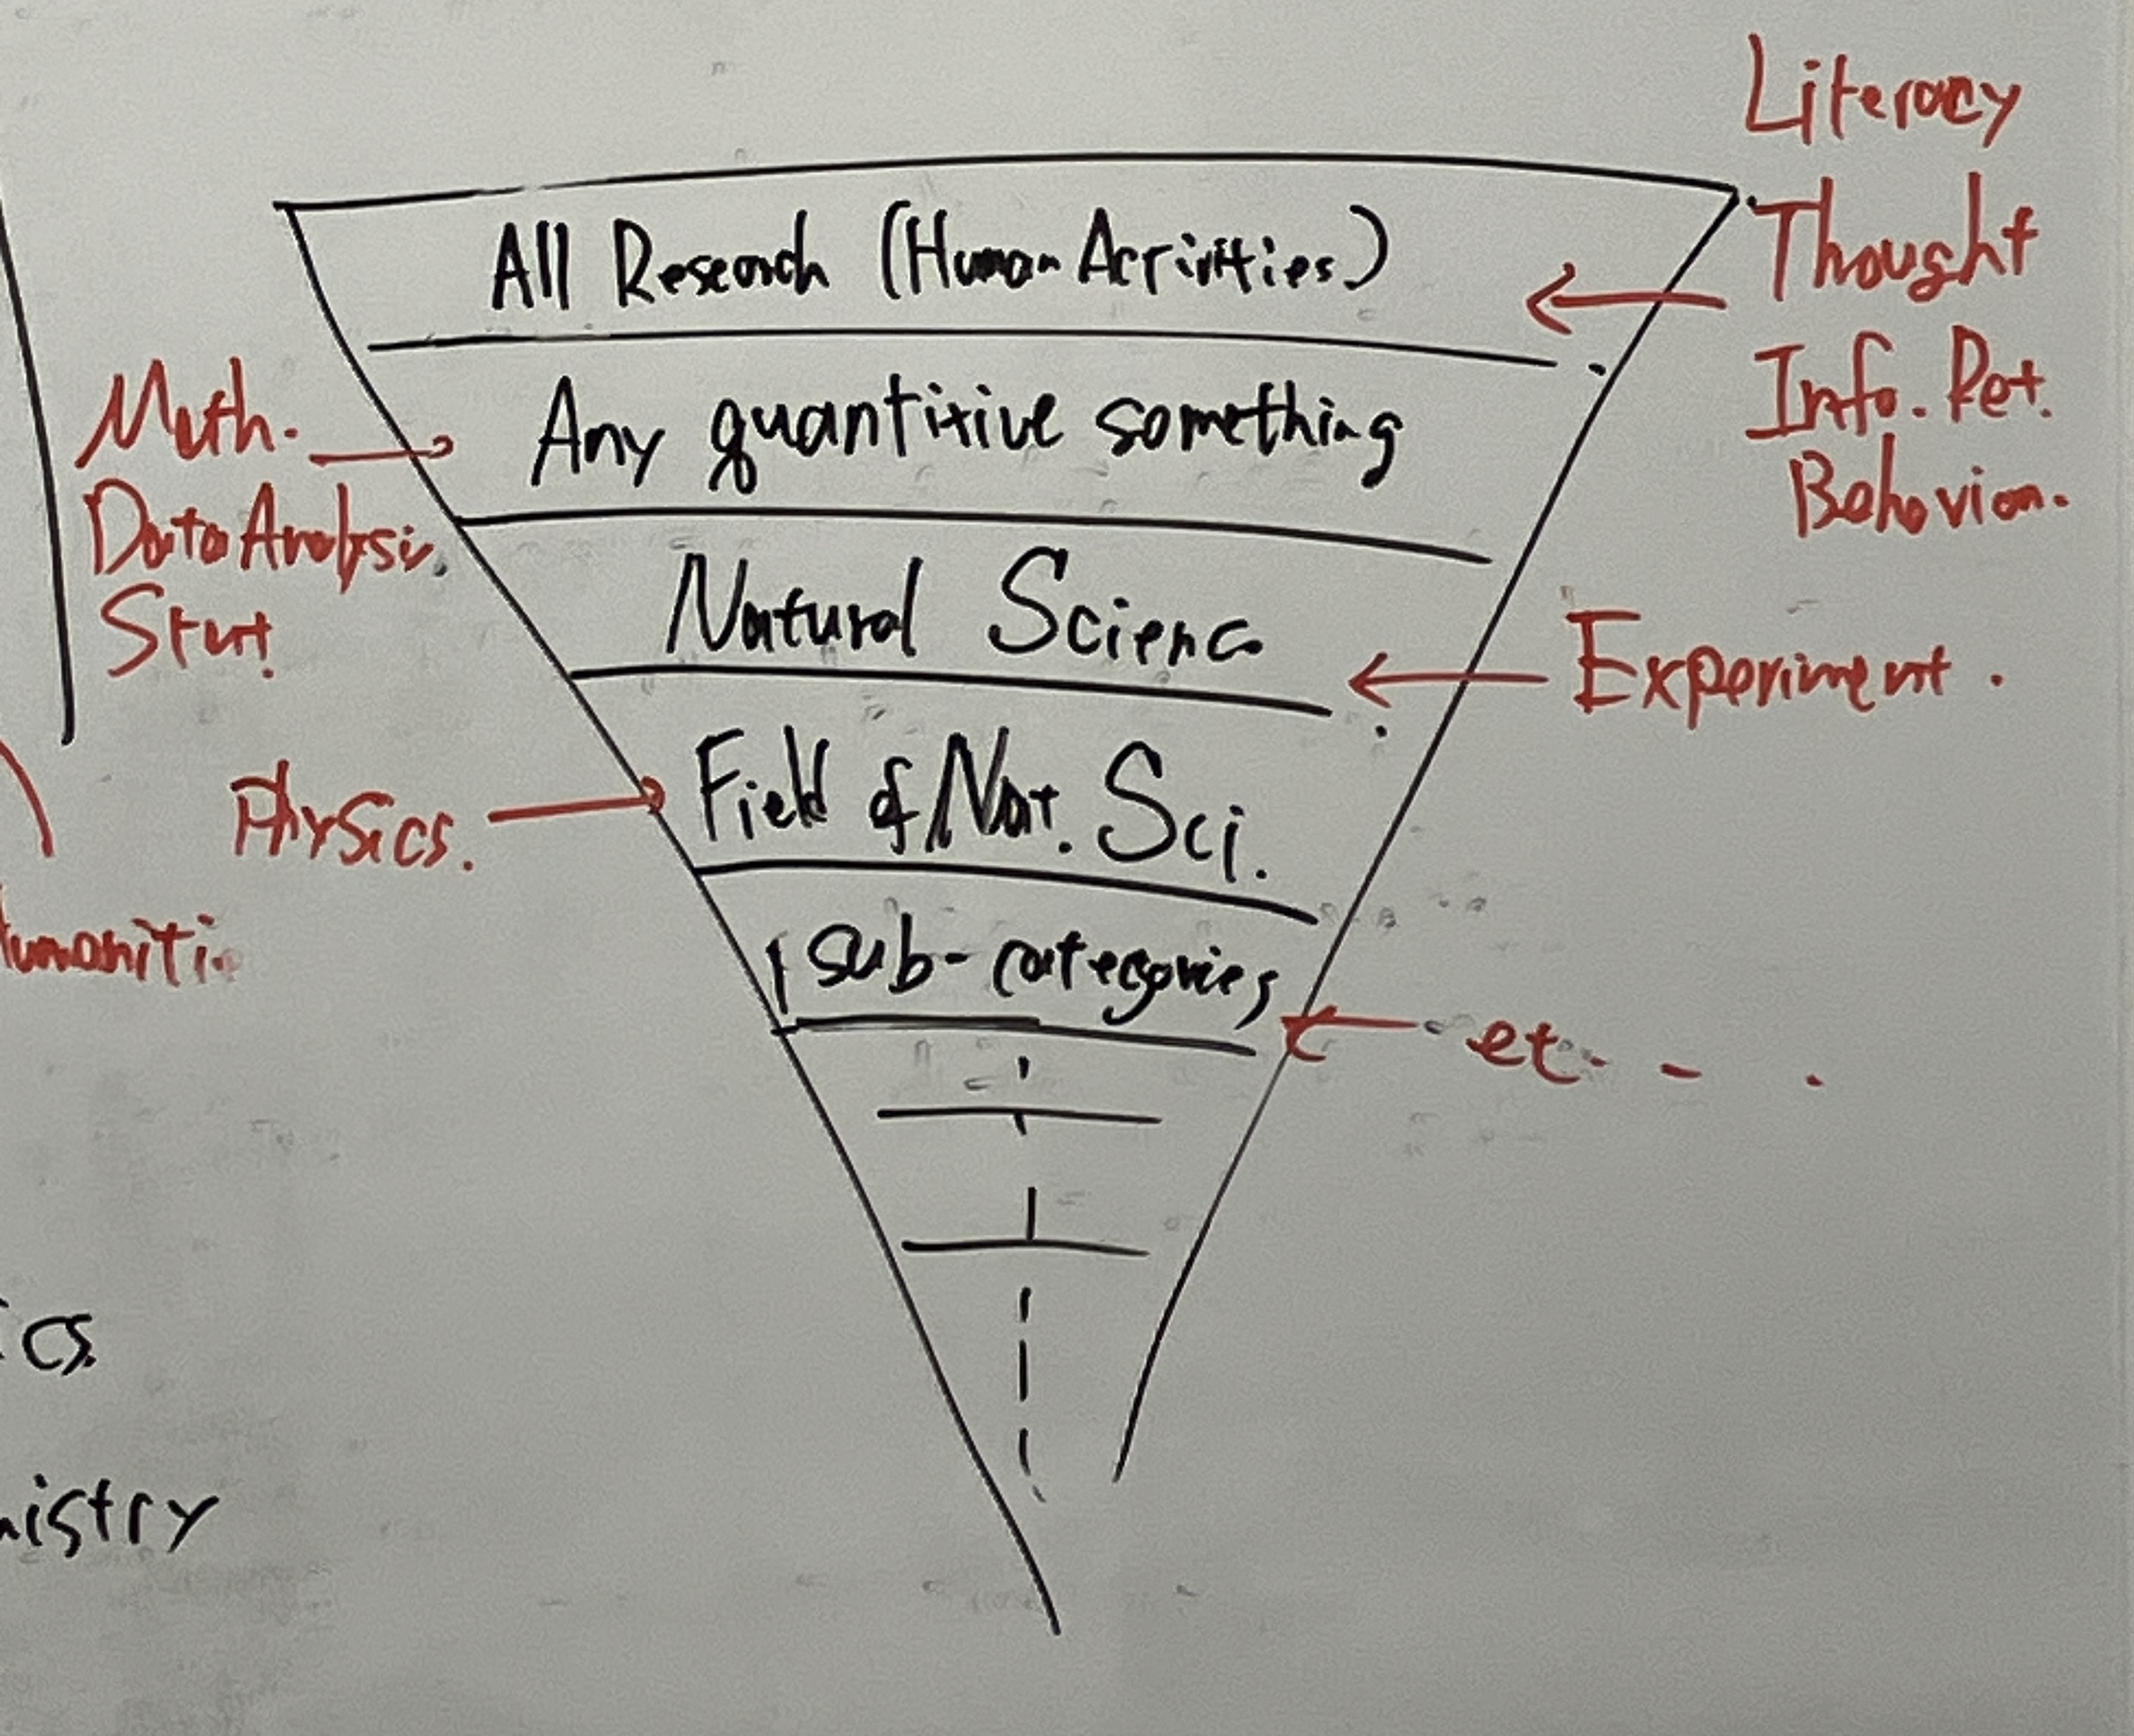
\includegraphics[width=\linewidth]{figs/generality_level.jpg}
    \caption{Caption}
    \label{fig:generality_level}
\end{figure}

% \section{Automation of Tasks for Diverse Field of Research}

% \subsection{Scholarly Document Processing}
% \textit{Scholarly document processing} is a general term for research on automated processing related to scholarly articles and has been studied as part of natural language processing, text mining, and information retrieval.

% \textcolor{red}{TODO: Skip for now. Need reconstruction because many of the issue discussed below are no more issue for research automation. Most of these will moved to Appendix}

% \subsection{Peer Review}
% Many studies have tried to automate peer review generation \cite{thelwall2019artificial,li2019generating,schulz2022future,yuan2022can,yuan2022kid,lin2021automated1,lin2021automated2,kumar2022investigations,bharti2022can,uban2021generating,wang2020reviewrobot}. While not generating peer reviews directly, studies focused on automating research paper assessment  can be said to be related to the peer review automation. \cite{kousha2022artificial,li2020multi,huang2018deep}. These studies have proposed the method to assess the quality \cite{thelwall2022predicting,thelwall2022can}, novelty \cite{pelletier2022novelpy,amplayo2019evaluating,shibayama2020measuring}, soundness \cite{cabanac2022decontamination}, and significance \cite{zong2022citation,xia2023review,soni2022predicting,manghi2021new,soni2021follow,van2020schubert,mckeown2016predicting}.

% These investigations concern the automation of processes occurring subsequent to a manuscript's arrival at the hands of reviewers. Conversely, researchers also have investigated the automation before that process, such as determining the appropriate journal for submission \cite{michail2023journal} and assigning the reviewers \cite{zhao2022reviewer}.

% While not centered on automation, certain studies engage in the scientific analysis of the review process \cite{shah2022challenges,verma2021attend,bharti2022confident,bharti2022betterpr,verma2022lack,kennard2022disapere}. These investigations serve to enhance our understanding of the nature of peer review and, in turn, provide valuable insights for the design of more effective automated review methodologies. 

% \subsection{Cognitive }

% \section{Automation of Tasks for Diverse Fields of Science}
% % There are prerequisite competencies and knowledge required to conduct scientific research. And the question of how to acquire such abilities has been one of the major concerns of AI research for science. Therefore, we will first introduce these research areas. In particular, we will present research on processing scientific literature and understanding scientific knowledge.

% % \subsection{Automated Theorem Proving}



% % \subsection{Understanding Scientific Knowledge}

% % \subsection{AI for Science}

% TODO

% \textcolor{red}{TODO: table for case studies to test the scientific understanding of chatgpt and gpt-4 }

% \subsection{Scientific Machine Learning: Inserting Inductive Bias for Scientific Understanding}
% Another prominent approach to incorporating such scientific knowledge into artificial intelligence is to incorporate inductive biases that help scientific understanding. This area has been studied typically under names such as \textit{scientific machine learning (SciML)} and \textit{physics-informed machine learning}.

% Whereas methods to learn scientific knowledge from the literature are generic methods that learn scientific knowledge through the generic interface of language, in this approach, humans add biases to either the model, the data, or the optimization method that are assumptions of scientific understanding. The constraints that have been studied include the abilities to handle (differential) equations, symmetry, intuitionistic physics, and so on \cite{hao2022physics}. 

% For differential equations, Physics-Informed Neural Networks \cite{raissi2019physics} and Neural Operators \cite{kovachki2021neural} are well known examples of this line of studies. These are methods that enable data-driven simulation of differential equations from data (forward problems) and differential equation discovery (inverse problems). Deep neural networks that can handle symmetry are studied under the name \textit{geometric deep learning} \cite{bronstein2021geometric}. The following survey is comprehensive in this area and should be referred to by those interested \cite{hao2022physics}.

% \subsection{For Empirical Studies}
% Research methods in science can be empirical or non-empirical. Empirical research is research that involves the generation of data, one of the crucial elements in science. Here, we present an effort to automate research on tasks related to scientific data. Machine learning is used in these areas in a variety of ways, including variable selection and model selection, but this section will focus specifically on those areas that have names.

% \subsubsection{Laboratory Automation}
% \textit{Laboratory automation} is a program that seeks to automate empirical research involving scientific experiments that involve interaction with the physical world.

% What makes this effort unique compared to other efforts to automate research is that it seeks to automate the entire process of validation, and it seeks to automate even the manual labor of humans in experimentation. Specifically, they automate human tasks by creating robots that can conduct research. A few examples include ``Mahoro'', a general humanoid robot that can conduct various experiments \cite{yachie2017robotic}. The robot could automatically conducted cell culture tasks using \cite{ochiai2021variable}

% \subsubsection{Bayesian Experimental Design}
% In order to conduct an efficient experiment, it is necessary to properly determine which experimental. \textit{Experimental design}, which involves devising efficient methods for conducting appropriate experiments, has long been studied. \textit{Bayesian experimental design} is an attempt to optimize and automate this experimental design by using Bayesian optimization \cite{chaloner1995bayesian,shahriari2015taking}. Bayesian experimental design has been incorporated from a relatively early stage and has been used in materials science and other fields.


% \subsubsection{Symbolic Regression / Equation Discovery}
% % \subsubsection{Symbolic Regression} 
% Scientists have constructed models in the form of mathematical equations that explain them from observational data. This has enabled us to go beyond observational data to understand and predict underlying phenomena. That is to say, formulating a mathematical representation that elucidates the phenomenon behind the data is an extremely critical step in science. 

% % Modern science is composed of a cycle of observation, hypothesis generation, and hypothesis testing. In many fields, including physics, chemistry, and biology, mathematical models are often constructed as hypotheses from observational data. 

% One attempt to automate this endeavor is \textit{symbolic regression} \cite{makke2022interpretable}, or \textit{equation discovery}. These are attempts to infer from the data a formula that explains it. While classical approaches to symbolic regression have traditionally employed methods such as evolutionary computation, recent years have seen the emergence of strategies utilizing deep neural networks \cite{petersen2019deep,udrescu2020ai,udrescu2020ai2,cranmer2020discovering,kamienny2022end,d2022deep}. Some researchers have proposed the frameworks \cite{landajuela2022unified,keren2023computational} and benchmarks \cite{matsubara2022rethinking} for symbolic regression. You can find a literature review of symbolic regression in \cite{makke2022interpretable}, and that of the early studies in \cite{kramer2023automated}.

% % \subsection{Knowledge Representation and Reasoning}

% \section{Automation of Tasks in Each Research Field}

% It has become commonplace to streamline domain-specific tasks in scientific research using machine learning, resulting in a vast number of published papers. Even just to mention a few that come to mind, there are studies on molecular biology \cite{jumper2021highly,senior2020improved}, material science \cite{ramprasad2017machine}, medical science \cite{vamathevan2019applications,shorten2021deep}, quantum mechanics \cite{carleo2017solving}, cosmology \cite{carleo2019machine}, genetics \cite{libbrecht2015machine}, and nuclear physics \cite{degrave2022magnetic}. It is impossible to cover all of these applied studies of research automation of science. Therefore, in this paper, we will not go into detail about each of these studies. Instead, we will present research on automation of elements that can be applied in various fields of science. For the literature survey of domain specific automation, please refer to \cite{xu2021artificial}. \textcolor{red}{TODO: Add application studies}

% \subsection{Automating Machine Learning}

% \subsubsection{AutoML}
% AutoML is an attempt to automate all tasks associated with machine learning. This includes hyperparameter optimization, model selection, and automation of various pre- and post-processing steps. The following website \cite{automlorg} provides a very active overview of AutoML. The book \cite{hutter2019automated} for an overview of AutoML through 2019, the paper \cite{bischl2023hyperparameter} for hyperparameter selection, and \cite{lindauer2020best,white2023neural} for the current state of the NAS are very helpful to catch up to this field.

% \subsubsection{MLOps}
% MLOps (Machine Learning Operations) is a general term for efforts to streamline and automate operations related to machine learning in industry. For example, it includes automating tasks such as model deployment and continuous training, as well as experiment management. To be sure, many MLOps solve problems in industry, and not all of them are related to research automation. However, when actually conducting research, we are involved in experiment management, versioning, and other tasks. While research on research automation has left out automation of these tasks, MLOps is accumulating knowledge on automation of these tasks as well.  The paper \cite{kreuzberger2023machine} is a good scientific review paper on MLOps.

% 
\tikzstyle{my-box}=[
    rectangle,
    draw=red,
    rounded corners,
    text opacity=1,
    minimum height=1.5em,
    minimum width=5em,
    inner sep=2pt,
    align=center,
    fill opacity=.5,
]
\tikzstyle{leaf}=[my-box, minimum height=1.5em,
    fill=orange!20, text=black, align=left,font=\scriptsize,
    inner xsep=2pt,
    inner ysep=4pt,
]
\begin{figure*}[tp]
    \centering
    \resizebox{\textwidth}{!}{
        \begin{forest}
            forked edges,
            for tree={
                grow=east,
                reversed=true,
                anchor=base west,
                parent anchor=east,
                child anchor=west,
                base=left,
                font=\small,
                rectangle,
                draw=red,
                rounded corners,
                align=left,
                minimum width=4em,
                edge+={darkgray, line width=1pt},
                s sep=3pt,
                inner xsep=2pt,
                inner ysep=3pt,
                ver/.style={rotate=90, child anchor=north, parent anchor=south, anchor=center},
            },
            where level=1{text width=5.6em,font=\scriptsize,}{},
            where level=2{text width=5.6em,font=\scriptsize,}{},
            where level=3{text width=5.5em,font=\scriptsize,}{},
            where level=4{text width=6.1em,font=\scriptsize,}{},
            [
                AI for Research, ver
                [
                    Natural Science, ver 
                    [
                            \cite{zhang2023artificial}{,}
                            \cite{xu2021artificial}{,}
                            , leaf, text width=46.8em
                    ]
                    [
                        Physics
                        [
                            \cite{carleo2017solving}{,}
                            \cite{carleo2019machine}{,}
                            , leaf, text width=39.7em
                        ]
                    ]
                    [
                        Chemistry
                        [
                            \cite{coley2020autonomous}{,}
                            , leaf, text width=39.7em
                        ]
                    ]
                    [
                        Biology
                        [
                            \cite{libbrecht2015machine}{,}
                            , leaf, text width=39.7em
                        ]
                    ]
                    [
                        Med. Science
                        [
                            \cite{vamathevan2019applications}{,}
                            \cite{shorten2021deep}{,}
                            , leaf, text width=39.7em
                        ]
                    ]
                ]
                [
                    Formal Science, ver
                    [
                        Mathematics
                        [
                            \cite{rabe2021towards}{,}
                            , leaf, text width=39.7em
                        ]
                    ]
                    [
                        Comp. Science
                        [
                            Contrastive~\cite{chalmers2013thing}{,}
                            POTTER~\cite{chalmers2013thing}{,}
                            CoT~\cite{chalmers2013thing}{,}
                            MCR~\cite{yoran2023answering}
                            , leaf, text width=39.7em
                        ]
                    ]
                ]
            ]
        \end{forest}
    }
    \caption{Review Paper of AI for Resear}
    \label{fig:categorization_of_reasoning_big}
\end{figure*}


% % \section{Another Axis: Research Process}
% % We have presented the idea that attempts to automate research could be classified hierarchically according to how broadly they could affect research. In addition to this, we believe that these efforts can also be categorized from another angle. That is, from the perspective of what part of the research process is being automated. For example, one effort might automate only the hypothesis generation part of a broad scientific study, while another effort might automate the entire research process instead of focusing on a specific research question. Also, for example, within an effort to automate validation, one effort might automate experimentation, another might automate proofs, and yet another might automate both of these. Thus, the second axis is what part of the research process is being automated and to what degree of generality.

% % Along this second axis, we will review our efforts in research automation. However, since there are a vast number of examples of research automation even in one sub-process, e.g., hypothesis generation, we will not go into individual details, but rather give priority to conveying the big picture.

% % % \textcolor{red}{NOTE: touch briefly do not go too specific, just show interpretation}
% % % \section{Knowledge Production}
% % % The Process of Creating New Knowledge

% % % Modern research is constructed from three main phases: observation, hypothesis generation, and hypothesis verification <- not line but cycle

% % \subsection{Question Construction}
% % In research automation studies, questions are often given. An exception is research that automatically discovers questions and issues from the academic literature. For example, Lahav et al. have proposed a methodology for automating the discovery of prevailing challenges within the research community, as well as the emerging hypotheses to address them \cite{lahav2022search}.

% % \subsection{Hypothesis Generation}
% % It is probably fair to say that hypothesis generation is one of the most common processes studied in research automation. Prediction of 3D structures from amino acid sequences, prediction of material structures from desired physical properties, and prediction of newly applicable disease candidates from existing drugs, just to name a few, are examples of automated hypothesis generation. In the example given in the previous section, symbolic regression is another example of hypothesis generation. These studies are often aimed at automation and optimization to solve bottlenecks in problems specific to each research area.

% % \subsubsection{Hypothesis Generation from Scientific Papers}

% % One study of automated hypothesis generation that is generic to a wide range of fields is the automatic generation of hypotheses from scholarly literature. In recent years, several researchers have presented studies on automating scientific analogical reasoning for identifying the relationship between problems and their corresponding solutions \cite{kang2022augmenting,chan2018solvent}, which is hypothesis.

% % % For example Portenoy proposed a system that recommend researchers who are pursuing analogous research objectives via divergent approaches \cite{portenoy2022bursting}.el techniques.

% % % \subsubsection{Others} 

% % Some methods have been proposed that don't generate hypotheses directly, but rather assist humans in generating hypotheses from experimental data 
% %  \cite{friederich2021scientific}.

% % \subsection{Hypothesis Verification}
% % Attempts to automate the verification of hypotheses include Bayesian experimental design, laboratory automation, and automated theorem proving, if theorems are viewed as hypotheses, as mentioned above. For example, some researchers have tried to automate experimental design for quantum physics \cite{ruiz2022digital} or proposed to design workflow of scientific research as a software \cite{goble2020fair}. Others have proposed machine learning algorithms for formulating and executing experimental designs in a more abstract and simple manner \cite{herrmann2022learning}. 

% % % \subsubsection{Verification Design}

% % % Once a hypothesis is formulated, a plan is developed to test its validity. The design of this verification plan is far more flexible than that of hypothesis generation, making it more difficult to handle uniformly. To be more precise, while many sciences have standardized methods such as statistical tests for verification, there is a wide variety of methods for generating the data used for the verification. One study may require a huge machine to collide elementary particles, while another may use rats for behavioral experiments. Some studies may require the use of chemicals, while others can be simulated on a computer. Furthermore, even with standardized statistical tests, as mentioned earlier, automating their creation from scratch proves exceedingly challenging. It is readily apparent that devising standardized methodologies like statistical tests is difficult when one must not merely employ them as tools but also contemplate the very nature of what it means to verify, as well as the rationale behind adopting specific assumptions. Therefore, it may not be an overstatement to say that this aspect represents the biggest obstacle towards achieving complete automation of research in a unified manner.

% % % \subsubsection{Verification Execution}

% % % Once a verification plan has been devised, the process proceeds in accordance with it. As previously mentioned, the approach may vary considerably. However, in many scientific methodologies, statistical techniques are employed. In these instances, the verification process can be broadly divided into two stages: 1. data generation and 2. analysis of the generated data for verification.

% % % As previously mentioned, data generation methods span a wide range. Among these, attempts have been made to automate the work of researchers within laboratories, an endeavor known as Laboratory Automation. For instance, 
% % % some studies focus on automating cell culture tasks using humanoid robots \cite{ochiai2021variable},
% % % TODO: add more

% % % TODO: may differentiate the analysis for hypothesis generation from that for verification
% % % we interpret data processed according to a certain criterion, assessing the validity of our inferences. Here, we make an explicit distinction between analysis for verification and analysis for hypothesis generation. Modern science is composed of a cycle of observation, hypothesis generation, and hypothesis testing. It's common to generate the next hypothesis to be tested from data produced for verification. However, this merely signifies that we conduct both hypothesis generation and testing through a somewhat inductive reasoning based on data. Therefore, in this context, we will focus on data analysis for hypothesis testing, while data analysis for hypothesis generation will be included in the hypothesis generation section introduced earlier.

% % To validate the plausibility of assertions, we currently employ statistical methods. There is research that automate the hypothesis testing \cite{gil2016automated}. 

% % Some researchers have engaged on automating data visualization and analysis \cite{bavishi2021vizsmith,bavishi2022tools}.

% % \subsubsection{Scientific Claim Verification}

% % Compared to question construction and hypothesis generation, there are few attempts to automate hypothesis verification related tasks from the academic literature. Somewhat related is the field of \textit{scientific claim verification} \cite{li2019scientific,wadden2020fact,wadden2022scifact,wadden2022multivers}, which determines the validity of a scientific claim through analysis of research paper. This is not the planning or execution of validation, but it is related to the automation of validation in the sense that it seeks to understand the validity of scientific claims. Since it is an assessment of the validity of a study, the findings of this study may have implications for the automation of peer-review.

% % \subsection{Pipeline (All Process)}
% % Most research on research automation automates some tasks in the research process. In contrast, there are attempts to automate the entire research process from start to finish.

% % \subsubsection{Self-Driving Labs}

% % A seminal early works are Adam \cite{king2004functional}, and Eve \cite{williams2015cheaper}. These are closed-loop scientific discovery systems that autonomously execute everything from hypothesis generation to research planning. These systems have logic AI at their foundation. The author of the paper of Adam call these system \textit{robot scientists}, \textit{self-driving labs}, \textit{autonomous discovery}, or \textit{laboratory automation}.

% % \subsubsection{Scientific Workflow}

% % Additionally, the concept of a \textit{scientific workflow}, which represents data and computational processing pipelines in research as software, emerged in the early 2000s. The developments and advances in research related to scientific workflows are consolidated in this literature \cite{barker2008scientific,atkinson2017scientific}. Additionally, these papers \cite{deelman2019role,nouri2021exploring} discusses how machine learning contributes to streamline the each step in the scientific workflow. These are important initiatives in terms of softwareizing the research process \cite{deelman2015pegasus,gil2011semantic}.

\subsubsection{Autonomy}

\subsubsection{General and Autonomous AI}

So far we have introduced the idea that we can look at research automation from two axes: the ``research field'' axis and the ``research process'' axis. We will try to paint a conceptual picture of how research automation can be viewed from these two axes.

\begin{figure}[htb]
    \centering
    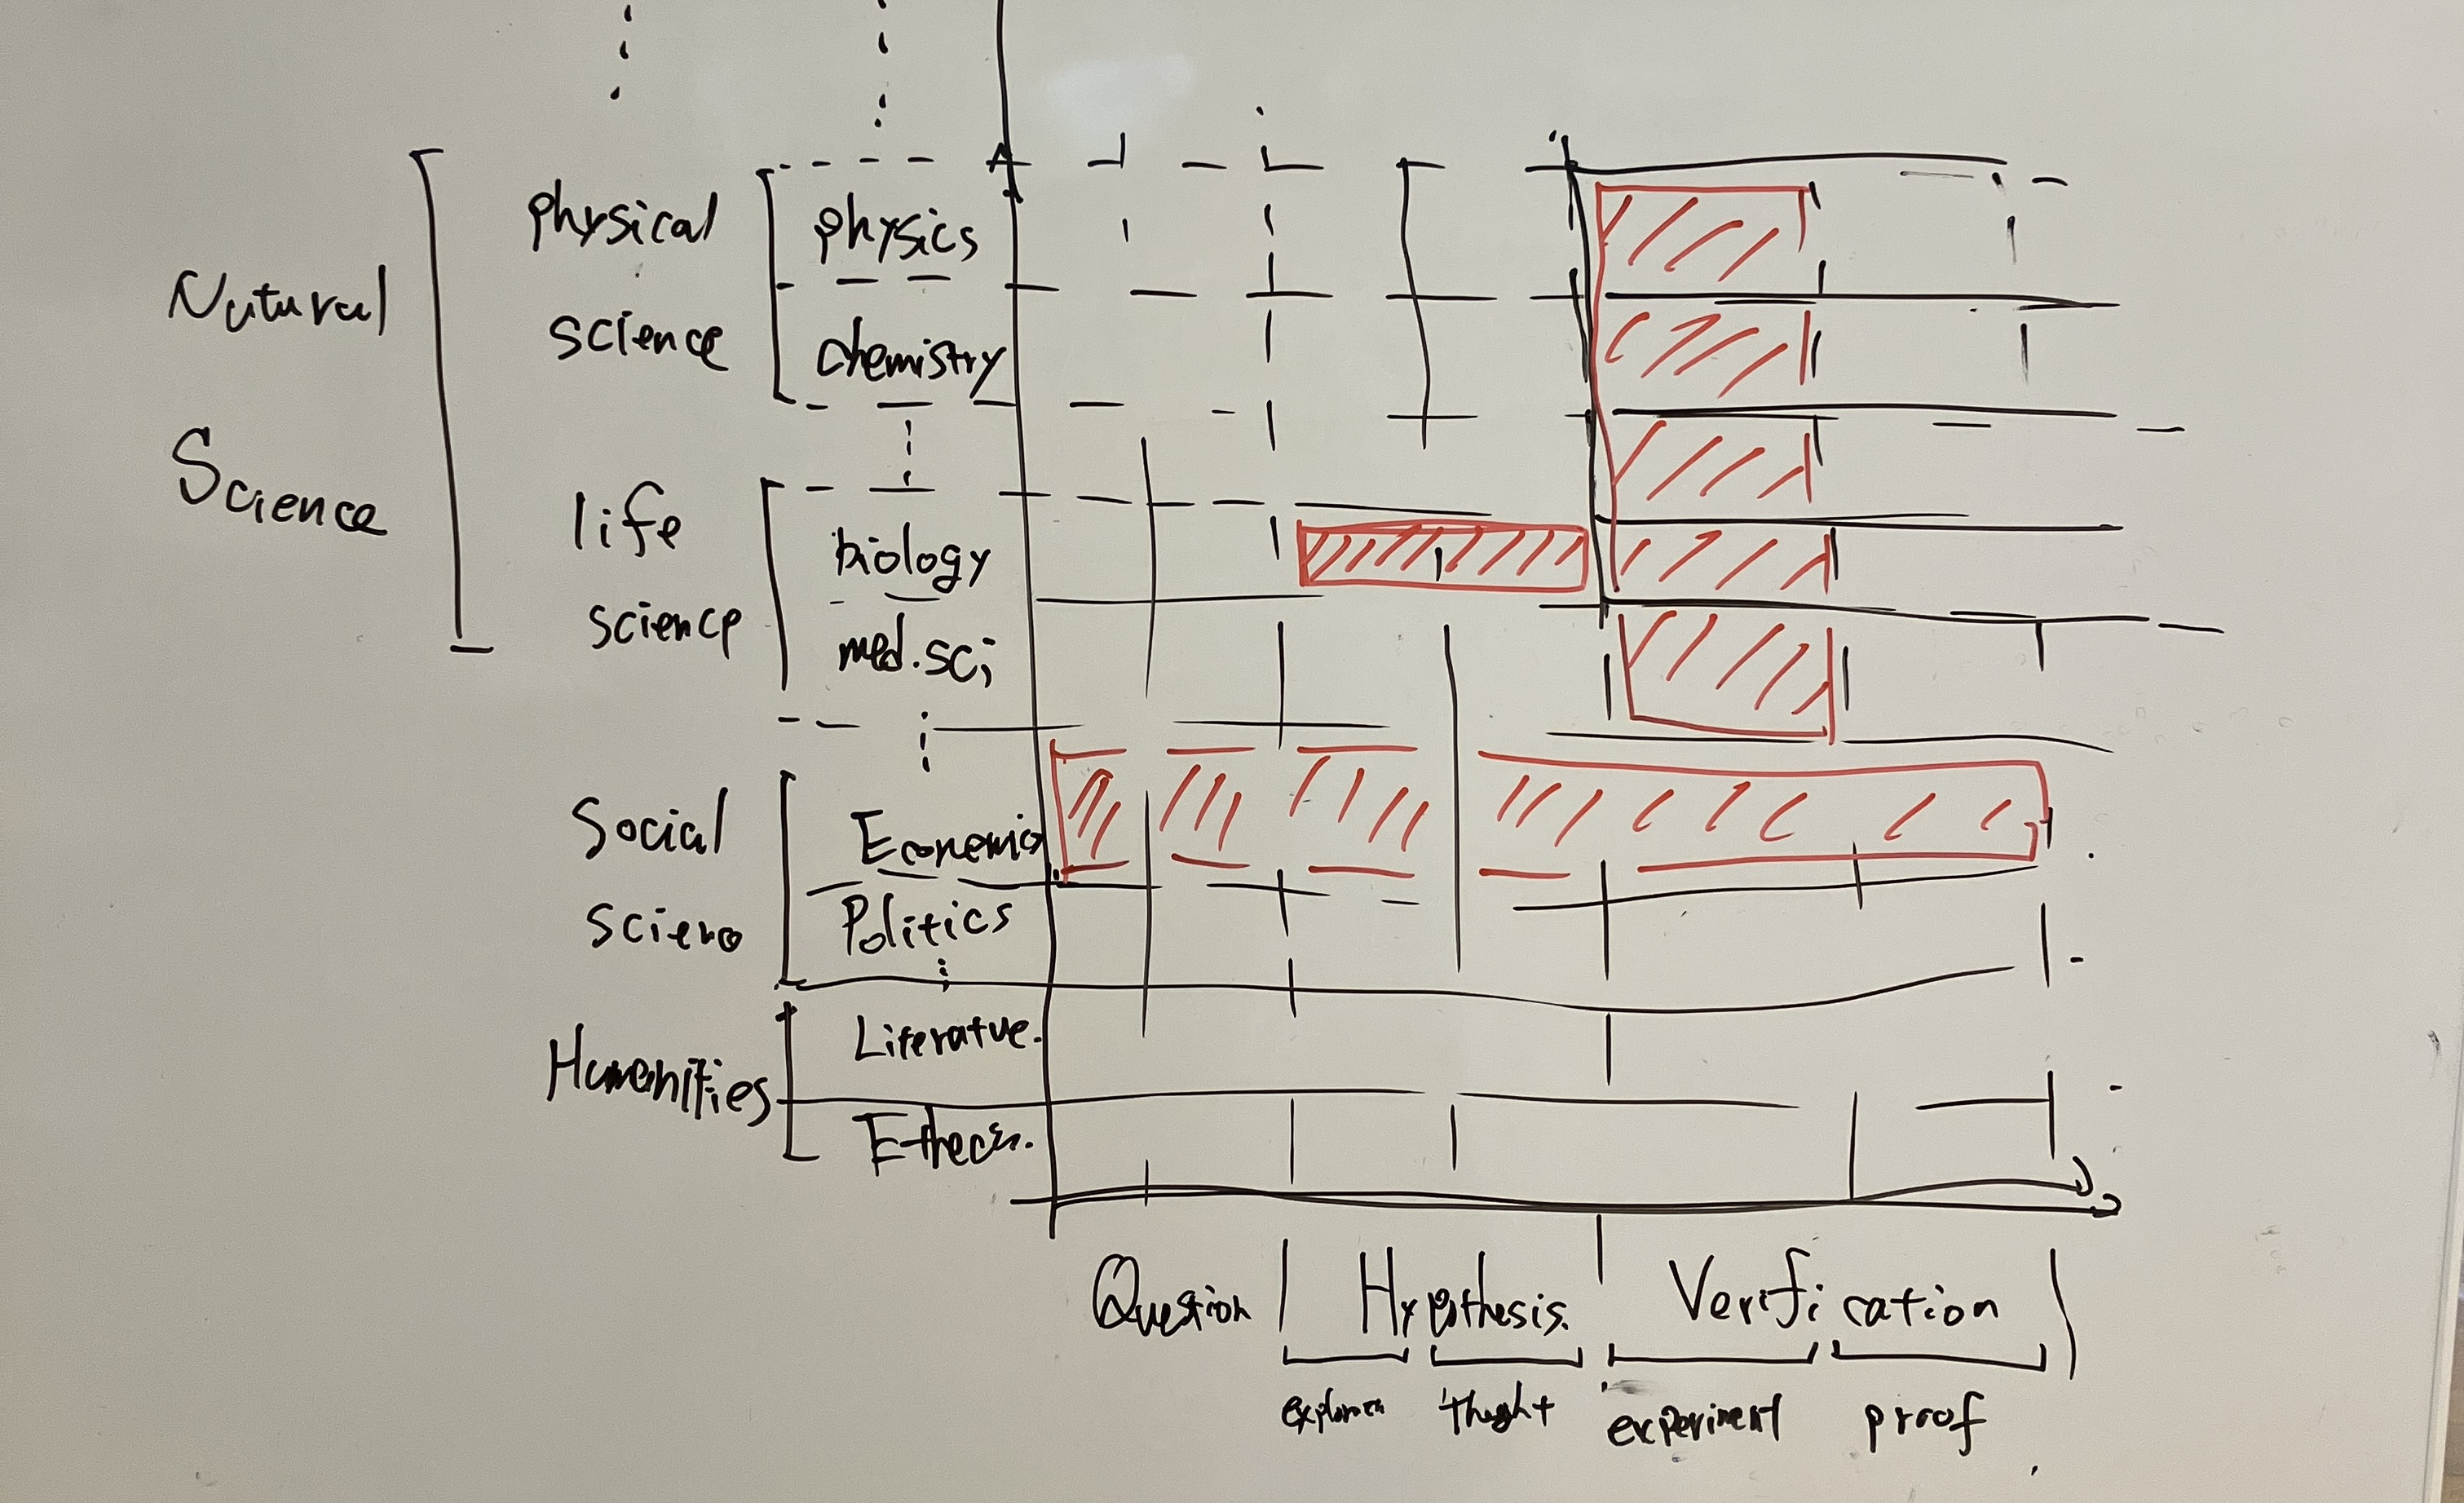
\includegraphics[width=\linewidth]{figs/generality_matrix.jpg}
    \caption{Caption}
    \label{fig:generality_matrix}
\end{figure}

Fig. \ref{fig:generality_matrix} conceptually illustrates the position of automation according to the axes of research field and research process. The vertical axis is the research field axis and the horizontal axis is the research process axis. Closer to the vertical axis corresponds to more specific research areas, and farther away from the vertical axis corresponds to a broader range of research areas. The horizontal axis corresponds to question construction, hypothesis generation, and hypothesis testing, from left to right, and is further divided within each category into more detailed e.g. empirical and non-empirical methods. Note that this is only a conceptual diagram and not an exact classification.

As a example, the automation of protein structure prediction \cite{jumper2021highly} can be seen as the automation of a certain hypothesis generation task in a certain molecular biology study. The work of robot scientist \cite{king2004functional} can also be understood as an attempt to automate many of the steps in the study of identifying the function of genes in genetics, from hypothesis generation, to testing, to generating new hypotheses. (Explanation of the figure).

Our goal of creating a versatile and autonomous artificial researcher is to automate everything on this two-dimensional surface. The area circled by the blue qualification in this figure corresponds to that. In other words, our goal is to realize an artificial intelligence that can autonomously execute any research or any process of research.



% \section{Others}

% Upon the completion of a study, the drafting of a manuscript, and its successful navigation of the peer-review process, the resulting findings are deemed to possess a degree of credibility as knowledge. Naturally, it would be hasty to assert that this alone births ``correct'' knowledge, as research demands iterative verification to confirm its validity. We convey such knowledge to others through various means, one of which is the presentation of research findings. To effectively communicate these outcomes, we create slides that elucidate our work. Studies also exist that strive to automate this aspect of the dissemination process \cite{sefid2019automatic}.

\section{Conclusion}

\section{Archive}

\subsection{Pursuing Better Research}
Please emphasize once again that what I are aiming for is to achieve a better way of knowledge production. The realization of general and autonomous artificial intelligence is a means to that end. Therefore, even if certain research practices are widely adopted at present, I will strive for better methods if they are not essential for knowledge production and if there are superior alternatives. In other words, I propose to pursue the realization of artificial intelligence that enables a different and improved way of knowledge production, rather than simply automating the current research practices.

While the practices of research developed by humans are highly sophisticated, robust, and productive, it is not necessarily true that all of them have reached the absolute optimum way of doing research. Firstly, research practices are strongly influenced by history and society. For example, peer review is widely accepted today, but it is said to have gained such dominant status because foundations in Cold War-era U.S. demanded peer review to ensure accountability \cite{baldwin2018scientific}. Moreover, the fact that research outcomes are still represented in the form of papers is clearly a remnant of the era when print was predominant. These practices might have been optimal under the social conditions and technologies of that time, but they may not necessarily be optimal in the present, as society has changed a lot. Additionally, meeting societal demands does not always lead to the optimization of knowledge production. Secondly, it seems that I sometimes lack a widely shared understanding of how to optimally carry out certain aspects of research. For instance, it is important to formulate good research questions and hypotheses, but there are still many aspects about how to do this effectively that remain unclear, and it appears to rely heavily on individuals' tacit knowledge. In such a situation, simply replacing current practices with machines may not guarantee a good knowledge production process. Thirdly, as Nielsen and Qiu say \cite{nielsen}, it is believed that I have only explored in a very limited subspace in the space of possible research practices. The establishment of current research practices is a very recent event in human history, and I may not yet have arrived at the optimum way of research. \textcolor{red}{TODO: Add examples.} Finally, as I mentioned above, current research assumes that humans are the main creators and consumers of knowledge. This naturally imposes human cognitive constraints, which may significantly limit the range of activities that can be conducted for knowledge production. Based on these reasons, I aim to progress the discussion in a way that allows us to identify what is fundamentally essential for knowledge production, while also drawing inspiration from the positive aspects of past practices. I will not be bound by the current approaches but instead strive to clarify what is truly crucial for research.

\subsection{Call for Cooperation}
I would be delighted if all of you could contribute to writing this research paper. The initial draft of this paper was created by a novice machine learning researcher named OO. I have made efforts to write the text as carefully as possible, but due to his limited research experience, He may not be able to provide profound insights into the topic, and there might be inaccuracies in his understanding of fields that are not his expertise. In particular, the literature review chapter prioritizes comprehensive coverage of the literature, which means that the evaluation of individual references might not be appropriate. Also, there are naturally limitations and biases regarding the scope of papers that can be covered and the research areas targeted. Therefore, if you find any errors, missed literature, or points for improvement in the paper, I would be grateful if you could let us know.



\subsection{Towards Understanding this Universe}
It has been a long-standing goal of humanity to understand nature, the universe, and the world. Through this intellectual curiosity, mankind has made remarkable intellectual advancements and uncovered astonishing findings about nature. While perfect understanding of this universe may be infeasible, the desire to know as much as possible about as many things as possible in this universe is a shared sentiment among researchers.

However, it seems that there are limitations to achieving this goal solely through current human capabilities. This is because humans have several cognitive constraints when it comes to understanding phenomena. For instance, there is a limit to the amount of information humans can process, and comprehending highly complex, nonlinear, and non-equilibrium systems in their entirety is challenging. Such constraints appear to narrow the scope of nature that can be understood. \textcolor{red}{TODO: update the explanation of cognitive limitation}

Furthermore, there is a possibility that the methodologies of knowledge production employed by humans currently may not be optimal. This is because the research practices I have developed are heavily influenced by historical and societal factors. Many of these practices have emerged in a relatively short span of history, and there is still a vast unexplored territory in the methods of conducting research.

We believe that artificial intelligence capable of autonomously conducting all research holds great potential in overcoming these challenges and getting closer to the goal. Firstly, AI is not constrained by a physical device like the human brain, enabling processing speeds and capacities that are orders of magnitude beyond human capabilities \cite{hope2022computational,kitano2021nobel}. Secondly, by optimizing AI for knowledge production, it becomes possible to generate knowledge more efficiently, without being constrained by extraneous factors commonly encountered in human research. Lastly, and most importantly, AI has the potential to possess a different understanding of nature compared to humans. Moreover, AI might have the capacity to comprehend nature more extensively than humans. If that's the case, it seems essential to develop autonomously researching artificial intelligence if one aims to acquire as much knowledge as possible about this universe. Therefore, I propose the pursuit of autonomous AI researchers to realize these possibilities.

\subsection{Objectivity of Research}

The objectivity of research seems to arise from such demand that knowledge should be for humanity. Because of this requirement, researchers conduct research with extreme precision and caution. This serves as one of the justifications for the knowledge produced through research being reliable. I admit that finding the basis of objectivity of research is a challenging philosophical issue. Please note that what I have stated here is merely the humble intuition.

Seeking public accessibility in knowledge implies that the expressions of knowledge and the process of knowledge production should be understandable to everyone. For instance, in human societies, knowledge is often expressed with texts. This is because language serves as a highly universal means of conveying information that a significant number of people can comprehend and handle. Similarly, the process of knowledge production is also conveyed through language.


% \section{Chapter Title}
\subsection{Scope of the Discussion}
I think that the activities related to research can be broadly divided into two phases: the process of knowledge production, typically in the form of papers or other publications, and the phase of maintaining, sharing, evaluating, and utilizing the knowledge. While the latter phase is a crucial aspect of knowledge, it will not be addressed here since the focus of this paper is on knowledge production. 

However, it's important to note that the distinction between the two phases is not strictly delineated. For instance, the value and usage of knowledge in a society would influence the production process of it, and research evaluation and revision are ongoing even after the knowledge is produced into the society. Thus, evaluation of the value of knowledge may not be completely exclude from my discussion simply because they mainly take place after knowledge production. As such, I will make sure to touch upon elements that are not always necessary for knowledge. 

Furthermore, factors influenced by social constraints such as funding acquisition and collaboration agreements that typically occur before the research are not addressed in this paper. Knowledge production can be seen as a function that produces knowledge from inputs such as people, capital, resources, and information. Viewing it this way, the acquisition of money or human capital can be considered inputs to the function rather than the knowledge production itself. Thus, I do not touch on this topic in this chapter. I admit that these factors are also crucial elements in the pursuit of true autonomy in research, so they will be subject to future discussions. Also, even if it is information acquisition, if that is strongly related to the internal of knowledge production itself, I will address it later in this paper. 

In conclusion, the following text focuses on the process of research, where knowledge is output as research outcomes given any input. For simplicity, I will refer to this process as the \textit{knowledge production system} or just \textit{research process}. It is worth reiterating that this distinction is provisional, intended to facilitate further discussion and the development of better categorizations or broader automation in the future.

\begin{figure}[htb]
    \centering
    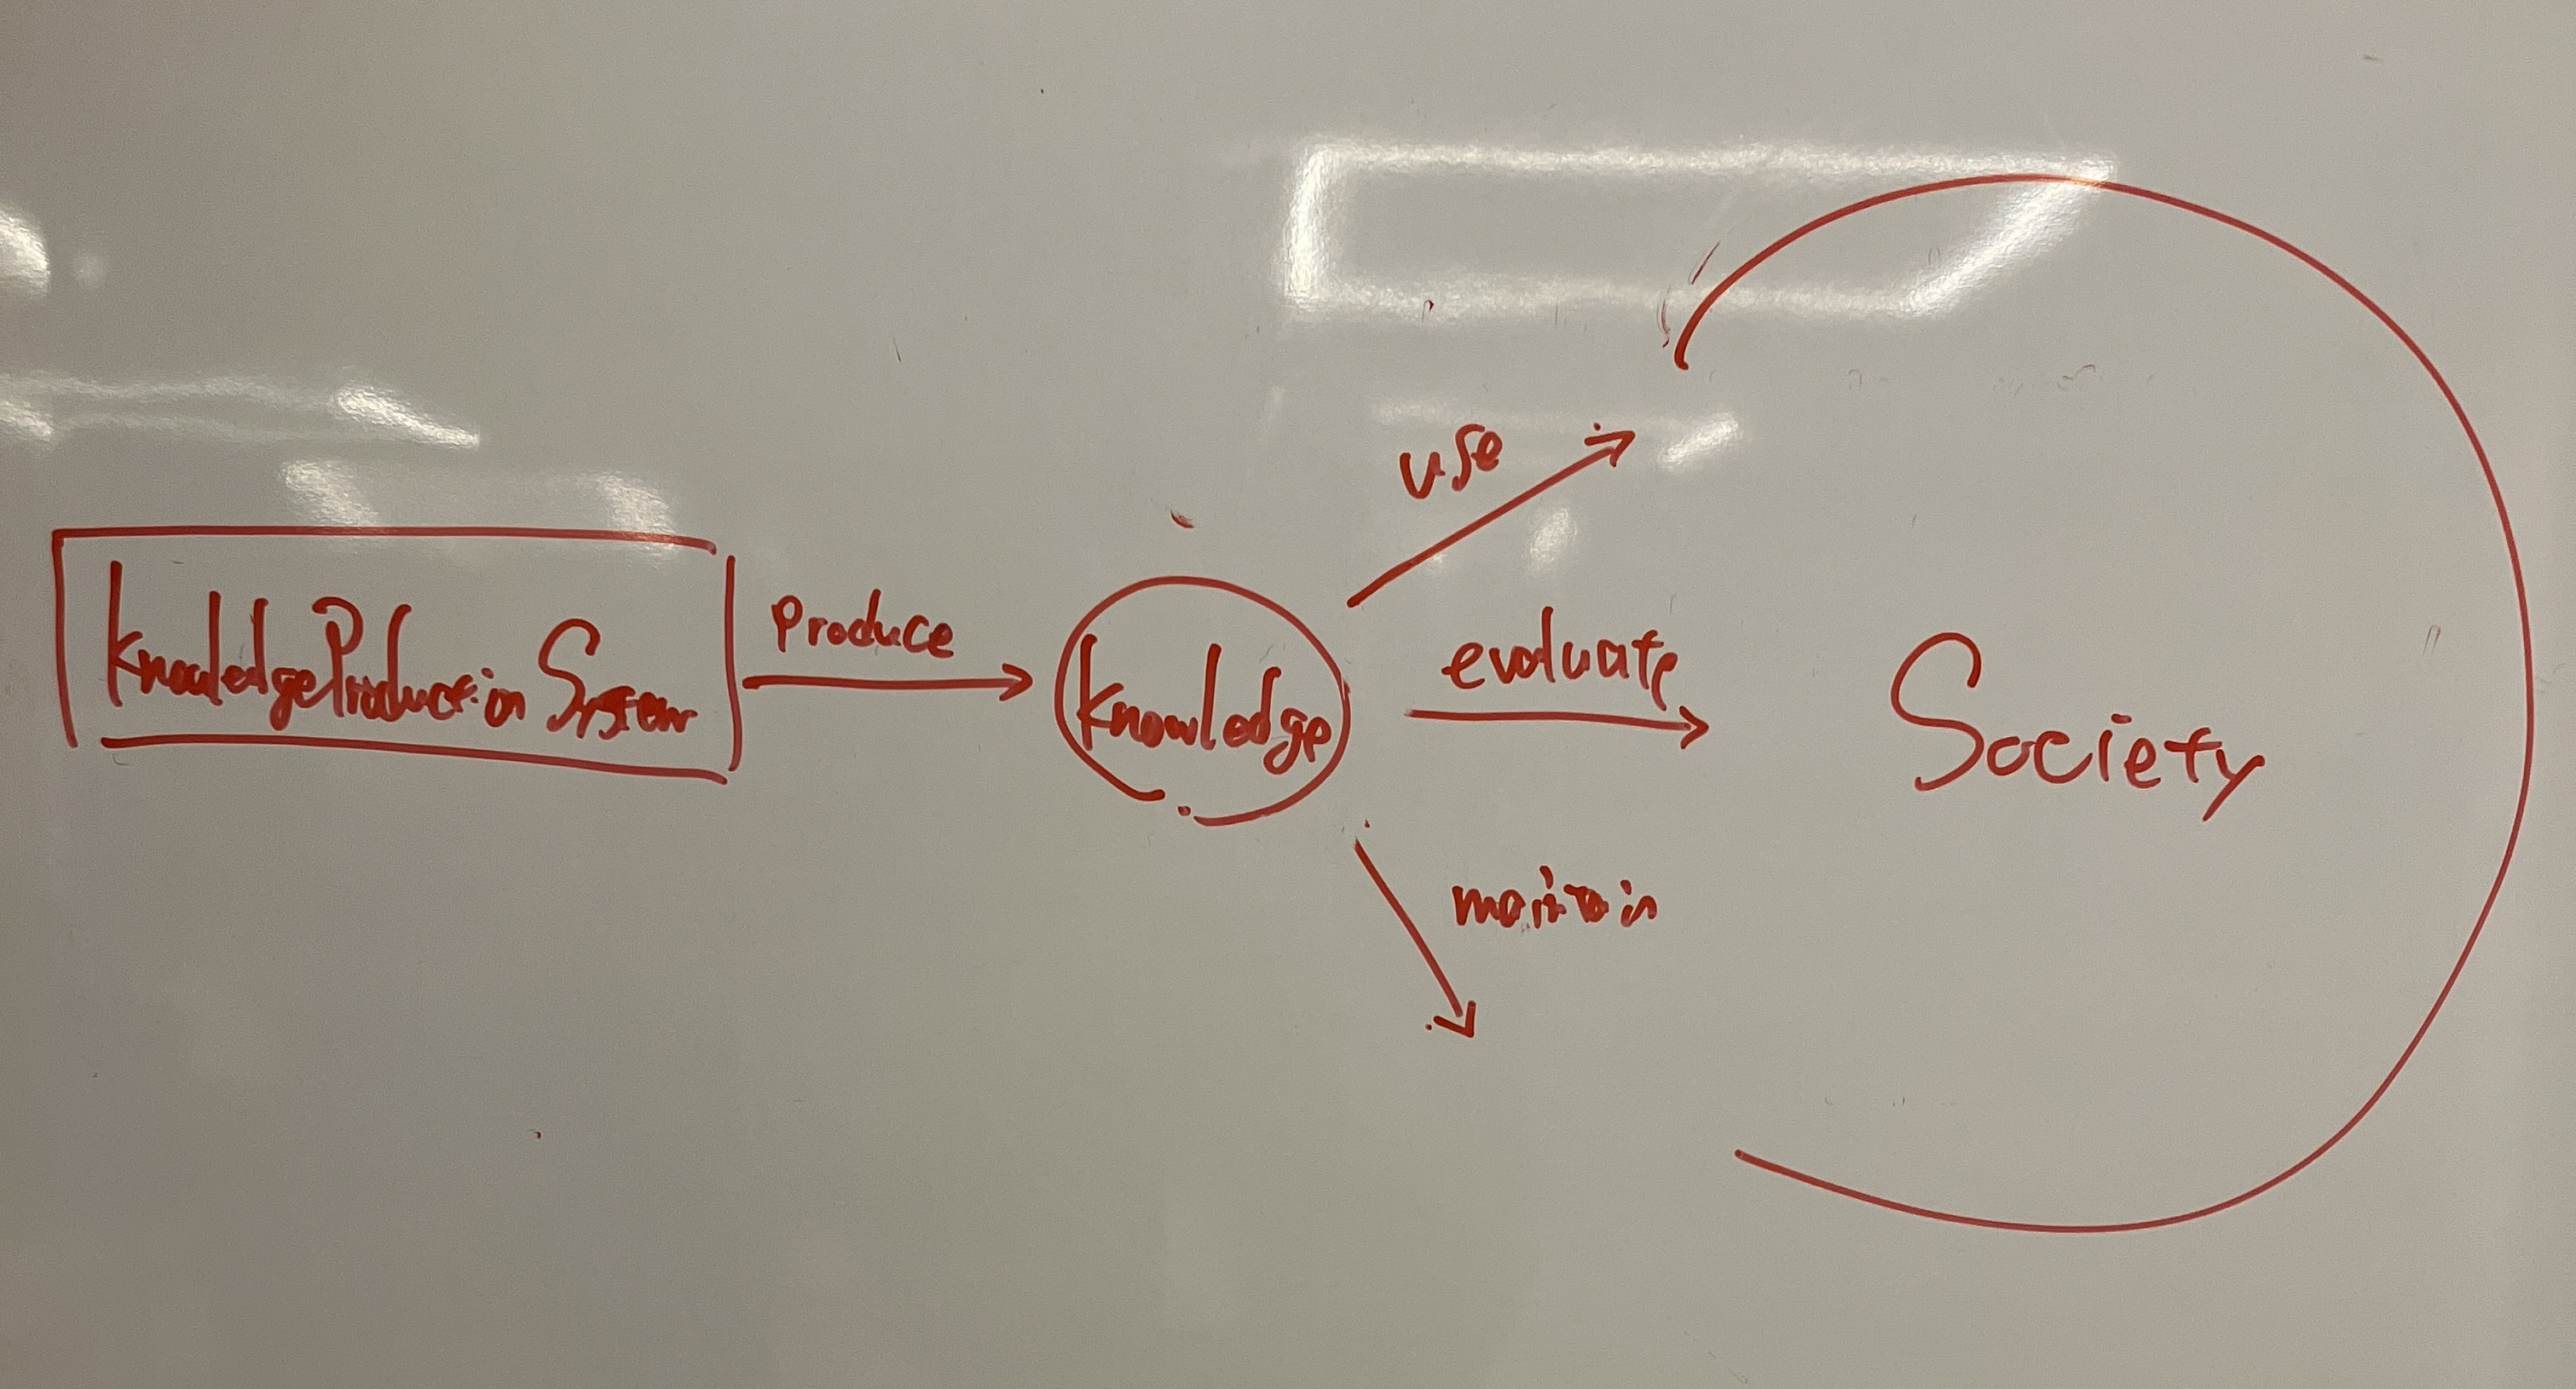
\includegraphics[width=\linewidth]{figs/research_process_society.jpg}
    \caption{Knowledge Production System and Society}
    \label{fig:research_process_society}
\end{figure}

\section{Research as Information Processing System}
Knowledge production system can be seen as an information processing system.\footnote{My discussion here is influenced by David Marr's three levels  \cite{marr2010vision}, although it is not exactly the same.} First of all, all information procesing systems have an objective and achieve that objective by processing inputs. In current case, the objective in research is to produce a new knowledge for a society. The reason I divided the research process into the question construction, hypothesis generation, and hypothesis verification is equivalent to breaking down this information processing into three sub-modules. Each of these three sub-modules is also an information processing system with its own objective. For example, the objective of the question construction module is to discover unknown knowledge.

When I have mention in this section that I would focus on the parts functionally related to knowledge production, it have meant two things. The first is to ensure that the objectives of these sub-modules are essential sub-objectives in all research. As mentioned earlier, these modules should not be something that works for history research but not for mathematics research. I should consider modules that have objective essential to all research for realizing general artificial researcher. Additionally, the process of peer review, while relevant to knowledge production, was considered to be a process of judging the ``value of knowledge'' and so was not included in the knowledge production system. The second point is that the my discussion is limited to the objective of the modules and not about the specific representation of information or the specific algorithms for information processing within the modules. For example, reading and writing papers are currently universally necessary for any research. However, a paper is just one of all representations of information, and there could be alternative representations (e.g., blogs). Moreover, while one person may conduct experiments using rats to verify a hypothesis, another person may present historical records showing statements from deceased individuals that match the hypothesis. These are different methods of verification, but both serve the purpose of verification.

% \textcolor{red}{TODO: Why this structurization is useful}

\begin{figure}[htb]
    \centering
    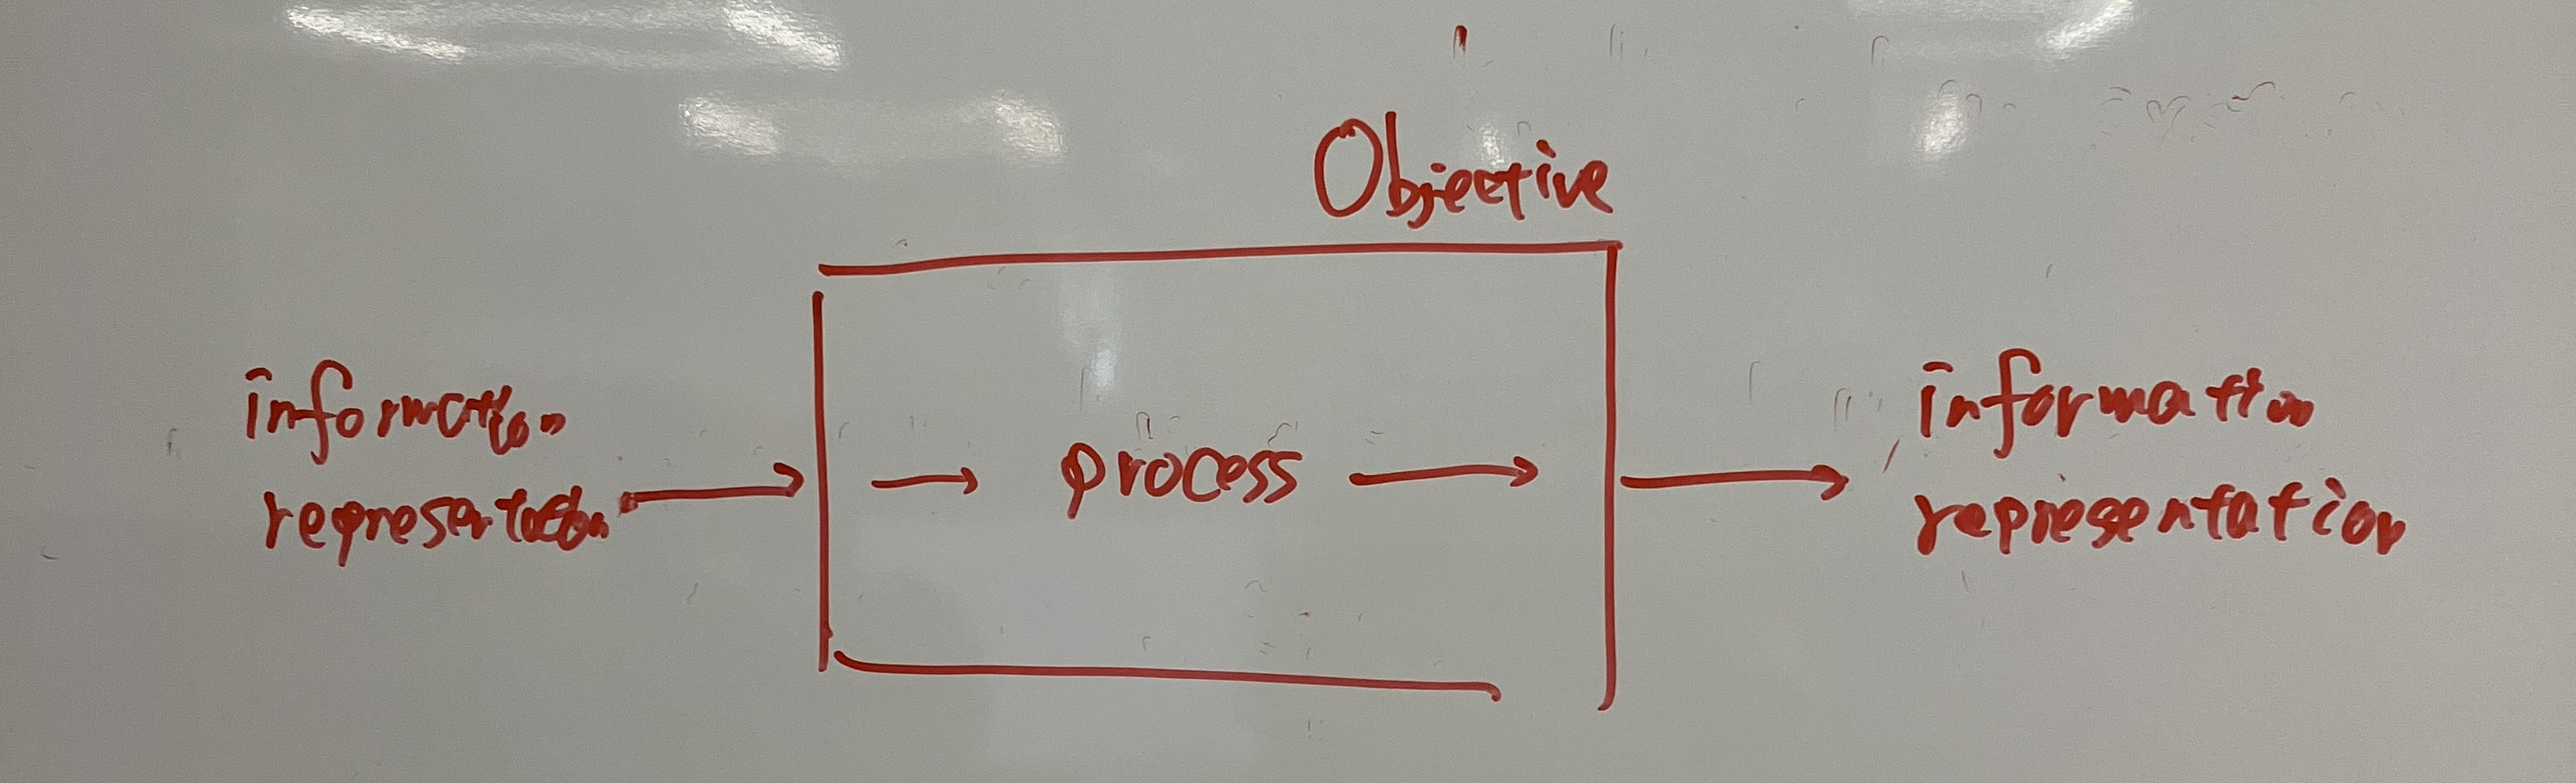
\includegraphics[width=\linewidth]{figs/information_processing_system.jpg}
    \caption{Knowledge Production System}
    \label{fig:information_processing_system}
\end{figure}

\begin{figure}[htb]
    \centering
    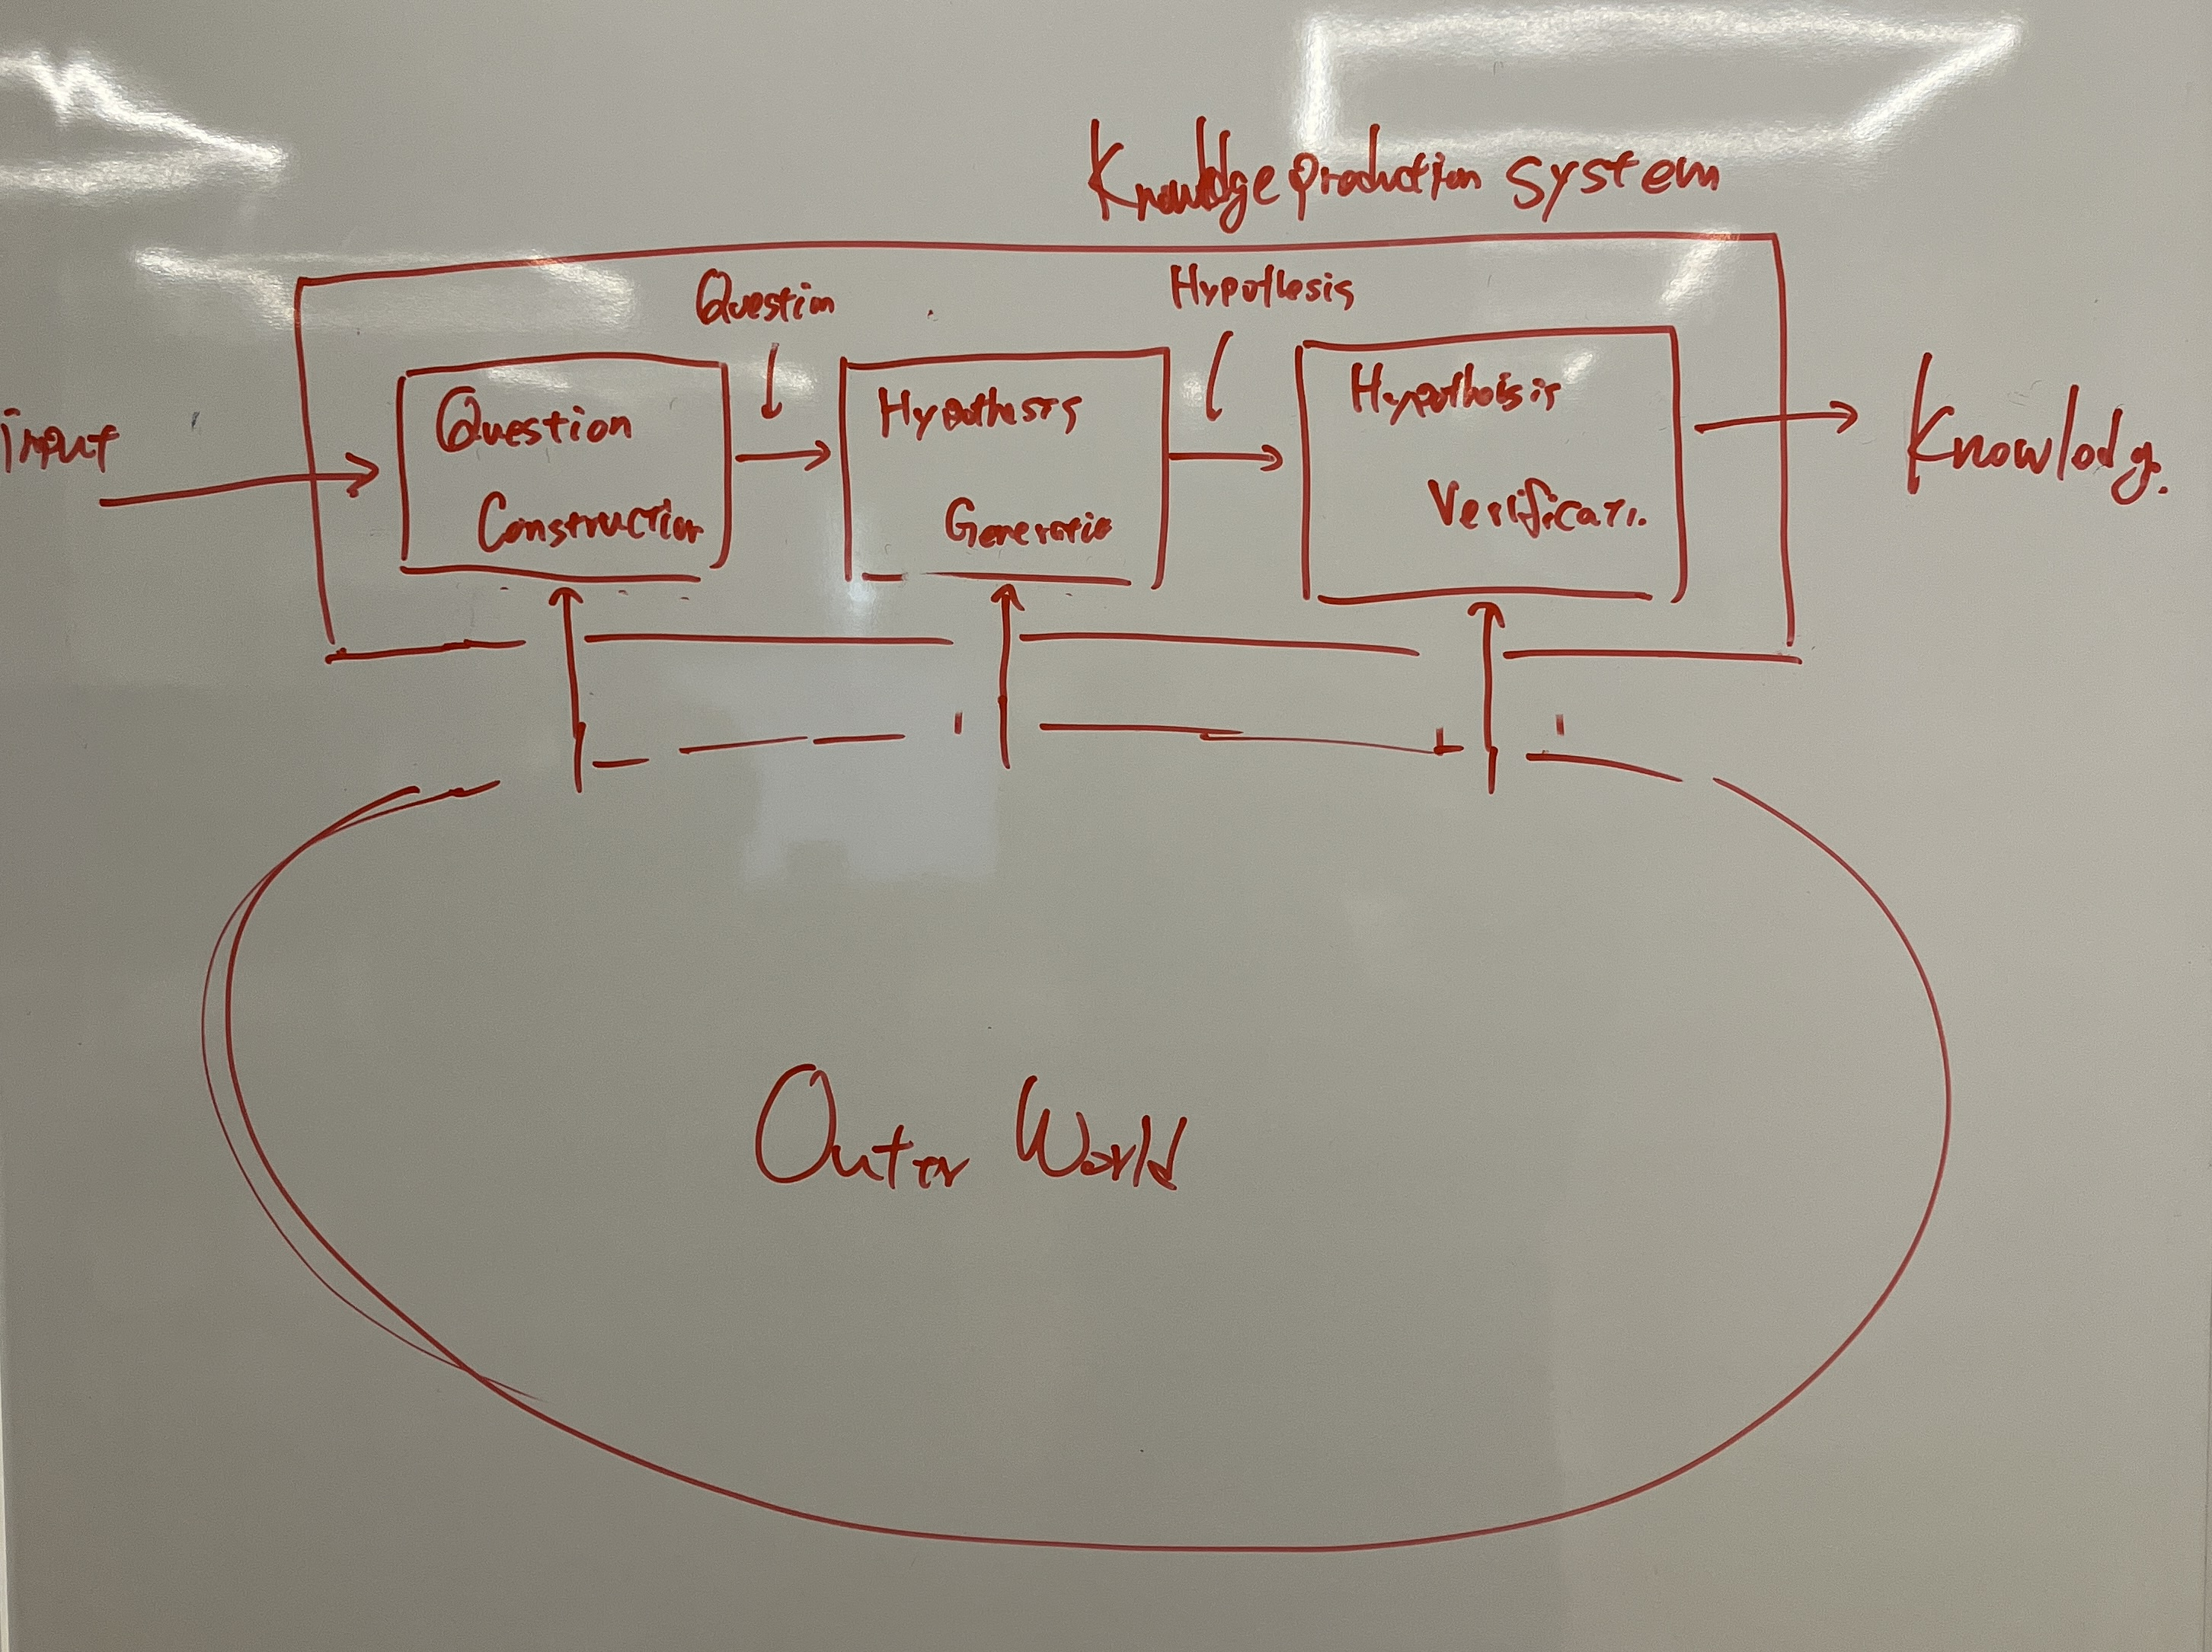
\includegraphics[width=\linewidth]{figs/knowledge_production_system.jpg}
    \caption{Knowledge Production System}
    \label{fig:knowledge_production_system}
\end{figure}

\section{Between the Knowledge Production System and Society}
In this section, I will discuss how peer review is related to knowledge production. The reason for discussing peer review is primarily because it is a widely practiced convention across various fields. I will discuss the role of peer review as a kind of membrane that spans both the preceding knowledge production and the subsequent knowledge utilization. I will also explore the possibility that the redundancy in the functions of peer review has played an essential role in the knowledge production of human societies. Lastly, I will discuss the implications of these conclusion for research automation.

% Peer review is a social convention developed in human societies.

% whether it is necessary or not for research, it is impossible to avoid discussing something that has been so widely accepted when considering research automation. 



\subsection{Peer Review}
In current research, a small group of experts review papers and the results that pass through their review are published. This process is called \textit{peer review}. Peer review is now considered an indispensable practice in research across a wide range of fields.

Peer review, particularly pre-publication peer review, is commonly regarded as playing the role of a gatekeeper of knowledge, determining what becomes knowledge and what does not. It enables the production of high-quality knowledge by assessing the quality before publication. Here, let's delve a bit deeper and examine the specific role that peer review plays in knowledge production.

\subsubsection{Epistemic Value Evaluation}

We believe that peer review serves two distinct roles in knowledge production. The first role is evaluating the fulfillment of necessary conditions for the knowledge of a research. This involves assessing aspects such as the validity of the methodologies used and the sufficiency of the content's novelty. 

This process could potentially be skipped if these evaluations were flawlessly conducted in every research endeavor during the knowledge production process. In that sense, I can say that peer review is redundant as a function for knowledge production, as it duplicates the functionality of what researchers have already done. If this process is merely redundant, does it mean that this process is unnecessary?

We would say that redundancy has played an important role in human knowledge production. Firstly, humans naturally make mistakes and have blind spots that they may not be aware of. It seems important to enhance the reliability of the produced knowledge by detecting such oversights with multiple checks. Secondly, research is fundamentally conducted on the assumption of goodwill, making it important to have a process to verify if any misconduct or ethical issues have occurred for the sake of a healthy knowledge production. Having a mechanism for third-party evaluation can be considered a deterrent against fraudulent activities. Lastly, as emphasized repeatedly in this paper, verification is an act of updating collective beliefs. Therefore, the existence of a process to confirm whether the verified results are acknowledged by others seems essential in the context of knowledge production for that society. Considering these factors, I believe that the first point, which functionally exhibits redundancy, has played an important role in human knowledge production.

\subsubsection{Non-Epistemic Value Evaluation}

The second role is about evaluating whether a proposed study has ``value'' to the research community and society. This involves judging factors such as the importance of the research, its clarity, and its ethical validity, etc. This function is obviously important as knowledge from research is supposed to be used by the research community and society.

This evaluation pertains to the submitted knowledge rather than the process of knowledge production itself. In a sense, it can be seen as an anticipatory assessment of the value judgments that will be made when the knowledge is disseminated in society. In other words, just as peer review was considered a redundant process in knowledge production for the first role, peer review can also be seen as a redundant process in terms of the judgments made on knowledge disseminated in society.

One role of redundancy in such judgments of social value would be to reduce the number of research results that knowledge consumers need to pay attention to. This has played an important role in human knowledge production, given the cognitive constraints of the limited number of papers that humans can process.

\subsubsection{Peer Review as a Redundant Membrane}

In summary, the first role can be interpreted as an extension of the knowledge production process, while the second role can be seen as a pre-emptive value judgment by society. In other words, the act of peer review serves as a redundant membrane that connects the process leading to the production of knowledge with the subsequent processes of knowledge use. \footnote{
In peer review, it is customary to assess whether there is sufficient information to reproduce the research. This evaluation of research reproducibility can be considered, in a sense, an assessment of its epistemic value. This is because, instead of evaluating the validity of verification through replication at that moment, the request for reproducible information aims to leave the possibility of future verification.
} Inspired by the words of Seetl, I can say that the former role is the judgement of \textit{epistemic value} and the later is that of \textit{non-epistemic value} \cite{steel2010epistemic}. 

Here, epistemic value refers to properties that are intrinsically important to knowledge production, such as necessary conditions for knowledge production. For example, I will call judging the validity of verification a judgment of epistemic value in the sense that it leads to judging whether the activity can be called knowledge production or not. 

The term non-epistemic value, on the other hand, is used in this paper to mean a value without which the legitimacy of knowledge production would not be affected. For example, if a knowledge production process were unethical, what it produced would still be knowledge, but it would be non-epistemic value in the sense that it is important to society. The readability or ``importance'' of a paper is also a use value of knowledge per se, but it has nothing to do with the legitimacy of knowledge production, so I call it a non-epistemic value. When I simply refer to ``value'' in this paper, I are referring to this no-epistemic value.

\begin{figure}[htb]
    \centering
    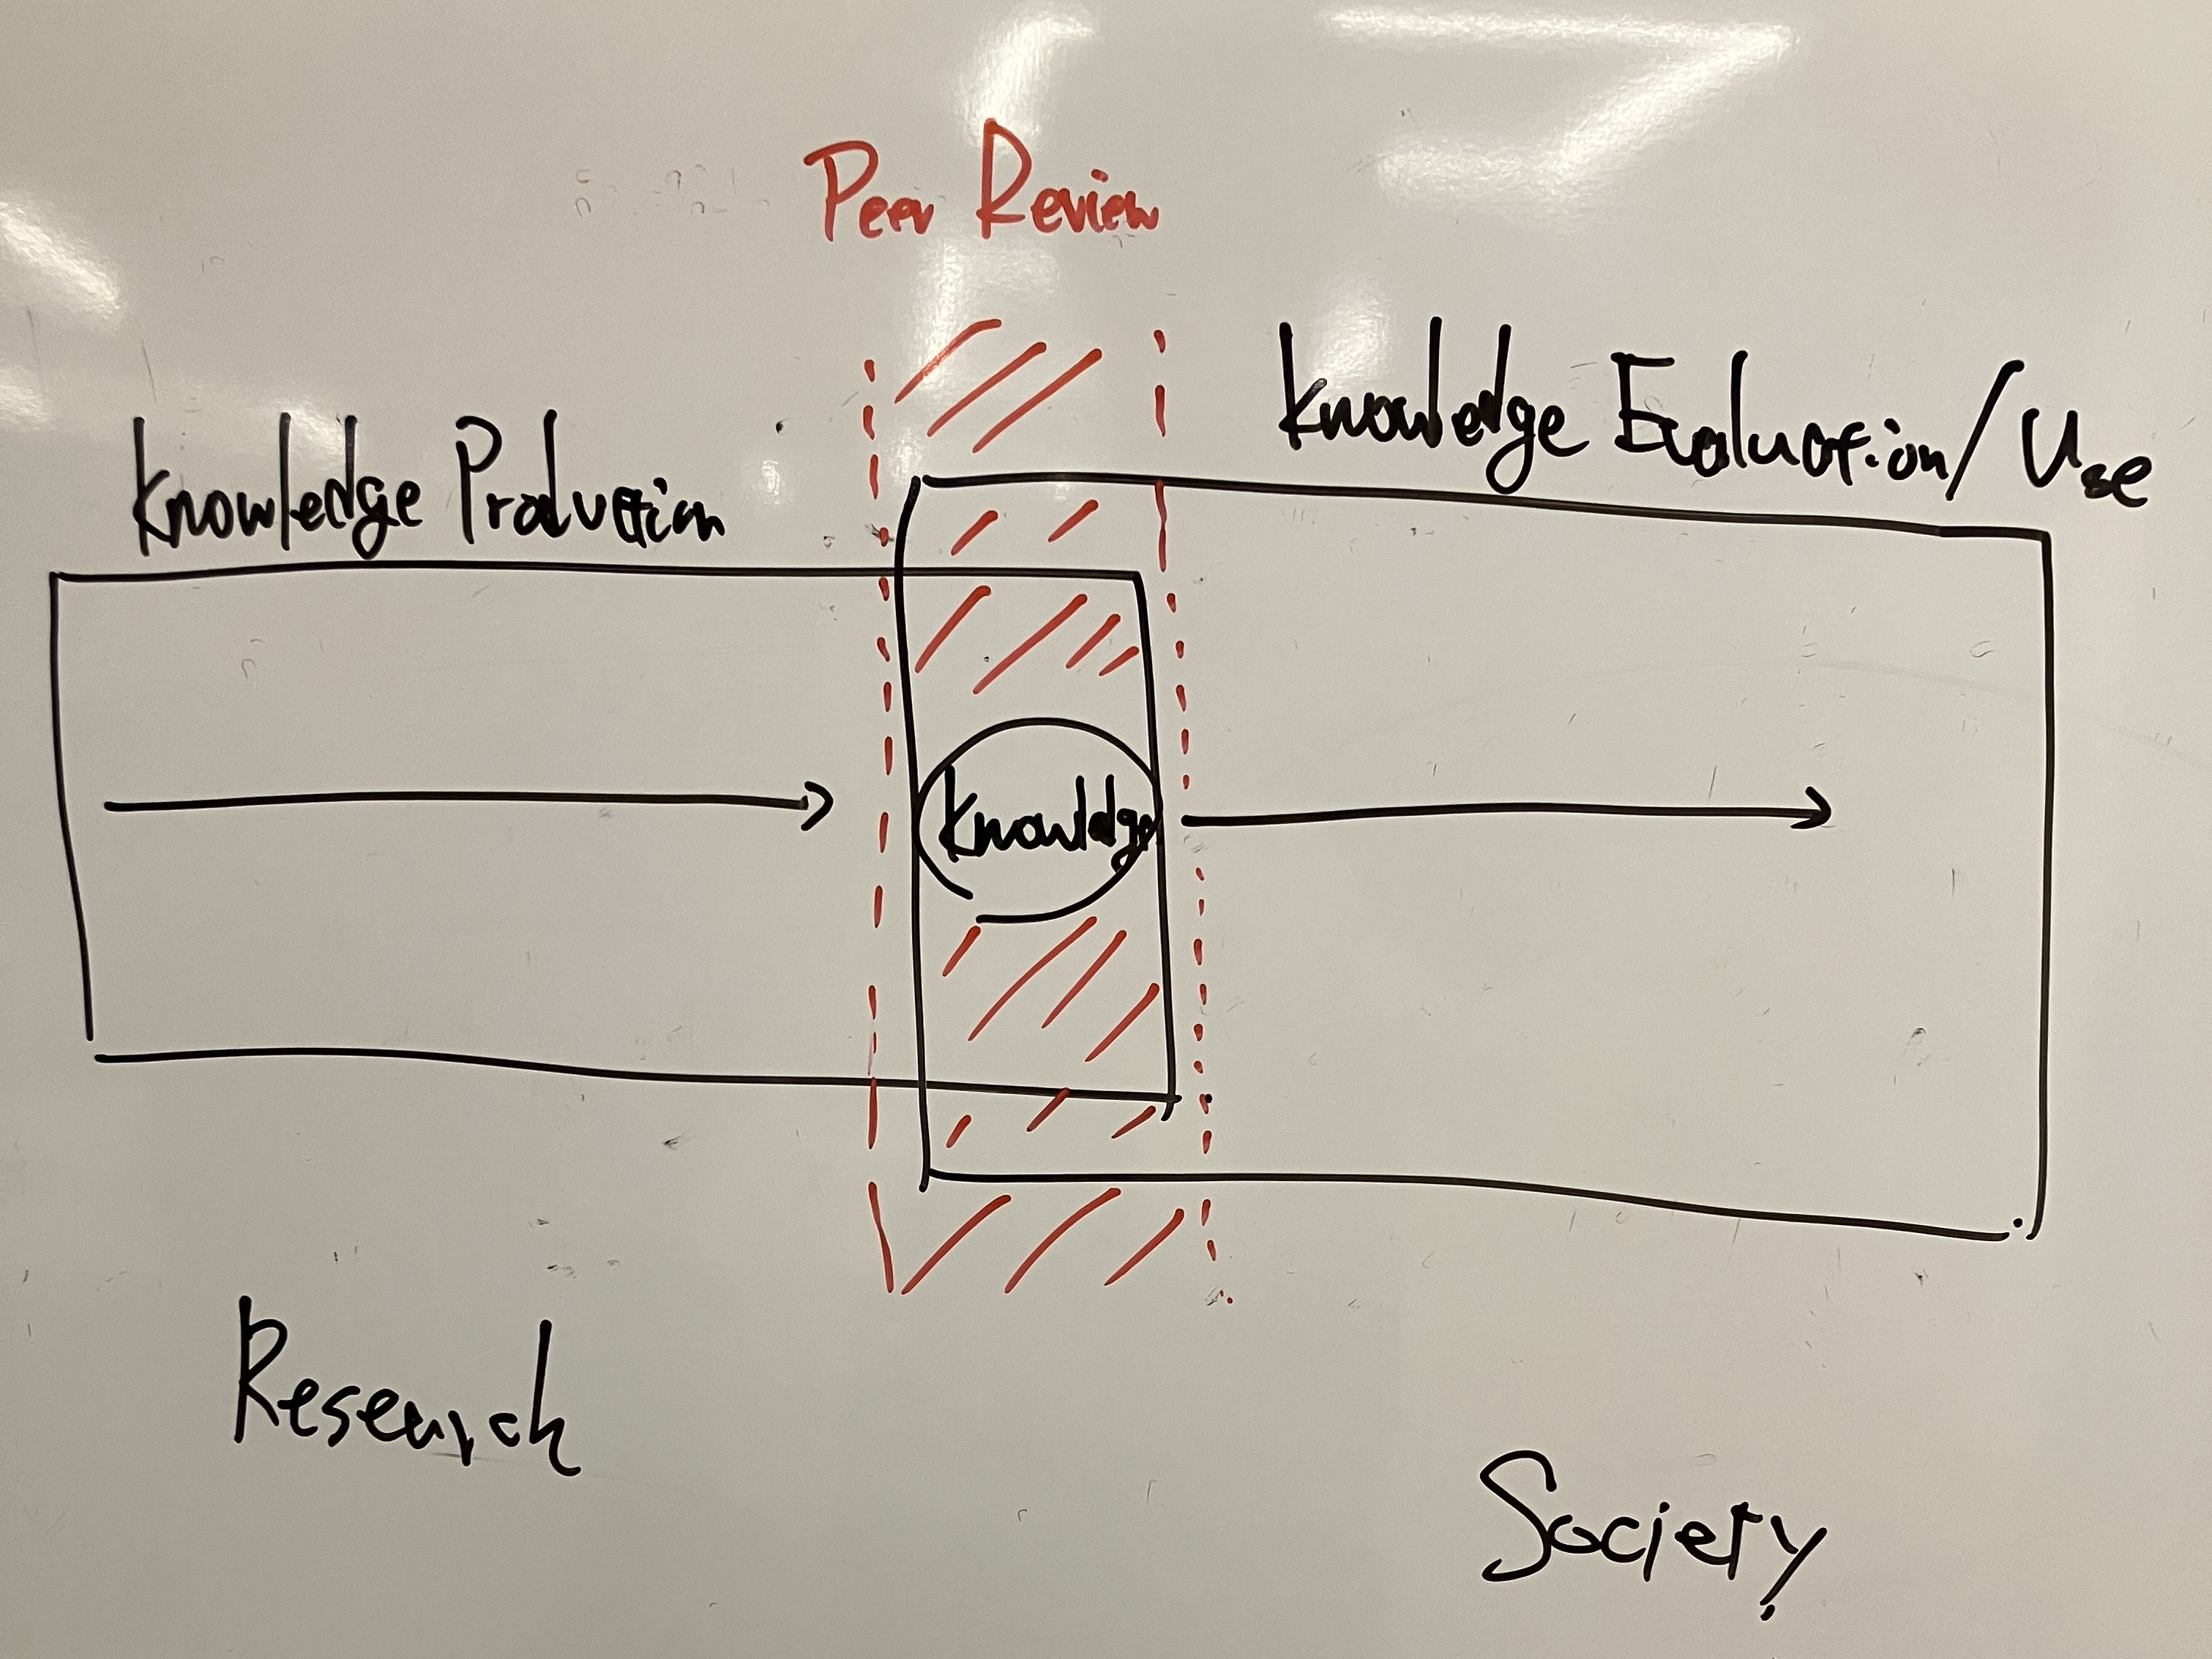
\includegraphics[width=0.8\textwidth]{figs/peer_review.jpg}
    \caption{Peer Review}
    \label{fig:peer_review}
\end{figure}

As an example, I show the review criteria of Nature in table \ref{tab:nature_review}. Each criterion is classified into epistemic value (evaluation of whether it fulfills the necessary conditions for knowledge production) and non-epistemic value (evaluation of whether it holds some value within the research community or society). From this example, it becomes evident that in peer review, research outcomes are evaluated from both epistemic and non-epistemic perspectives. 

\begin{table}[H]
\centering
\begin{tabularx}{\textwidth}{|X|X|X|}
\hline
\textbf{Criteria} & \textbf{Category} & \textbf{Explanation} \\ 
\hline
Key results & NA & Please summarise what you consider to be the outstanding features of the work. \\ 
\hline
Validity & Epistemic & Does the manuscript have flaws which should prohibit its publication? If so, please provide details. \\ 
\hline
Data \& methodology & Epistemic & Please comment on the validity of the approach, quality of the data and quality of presentation. Please note that I expect our reviewers to review all data, including any extended data and supplementary information. Is the reporting of data and methodology sufficiently detailed and transparent to enable reproducing the results? \\ 
\hline
Appropriate use of statistics and treatment of uncertainties & Epistemic & All error bars should be defined in the corresponding figure legends; please comment if that’s not the case. Please include in your report a specific comment on the appropriateness of any statistical tests, and the accuracy of the description of any error bars and probability values. \\ 
\hline
Conclusions & Epistemic & Do you find that the conclusions and data interpretation are robust, valid and reliable? \\ 
\hline
Suggested improvements & Epistemic & Please list additional experiments or data that could help strengthening the work in a revision. \\ 
\hline
References & Epistemic & Does this manuscript reference previous literature appropriately? If not, what references should be included or excluded? \\ 
\hline
Originality and significance & Non-epistemic & If the conclusions are not original, please provide relevant references. On a more subjective note, do you feel that the results presented are of immediate interest to many people in your own discipline, and/or to people from several disciplines? \\ 
\hline
Clarity and context & Non-epistemic & Is the abstract clear, accessible? Are abstract, introduction and conclusions appropriate? \\ 
\hline
Inflammatory material & Non-epistemic & Does the manuscript contain any language that is inappropriate or potentially libelous? \\ 
\hline
\end{tabularx}
\caption{Nature Review Criteria}
\label{tab:nature_review}
\end{table}

\subsubsection{Implications for Research Automation}

If peer review is considered redundant in knowledge production, then the necessity of the peer review process when conducting research with artificial intelligence, which may have fewer cognitive constraints than humans, becomes a topic of discussion. If there are no occurrences of human errors, it may not be necessary to have a redundant process. So is peer review simply a social product of human cognitive constraints, or does it play an important role in knowledge production even in automated research?

We believe the importance of redundant valuations will not be lost in automated research. First, regarding the function of detecting oversights, automating research may eliminate certain types of mistakes, but overlooking aspects is still possible. For instance, as mentioned earlier, it is impossible to enumerate all the assumptions involved in the research process. Review could help by identifying relevant assumptions that need consideration, potentially altering the implications of the validation results. Second, against malicious injustice, this also happens in the automated research as well. There is a possibility of creating artificially intelligent researchers that could maliciously manipulate and engage in fraudulent activities. Furthermore, in the ultimate stage of full autonomy, as pointed out in alignment research, there is a potential for machines to deceive humans as well. Also, since the goal remains the same, whether the research is done by humans or by machines, to update joint beliefs, it is just as important that it is actually evaluated by other members of society. Finally, in the first place, the nature of research is that hypotheses are continually subjected to constant testing. As mentioned earlier, a hypothesis tested by inductive reasoning cannot be declared true in the same way that deduction can. It is common for the knowledge to be later discovered to be erroneous or merged with other new knowledge. Therefore, it seems to me that this redundant process of criticism is essential for research, and should not even be imposed on a single process of peer review. For these reasons, it would seem that redundant evaluation from a third-party perspective should somehow be accomplished even in automated studies.

From a slightly different perspective, aiming to automate peer review of papers may be a useful first step toward generic and autonomous research automation. This is because peer review involves judgments about the validity of verification, as well as judgments and novelty determinations, factors that I have emphasized as important in research automation. Moreover, while finding novelty and performing validation are generative tasks, this is an classification task, and in that sense it is an easier task. Similarly, I pointed out that it is important to inculcate the value of what is important to the research community if I want machines to construct ``important'' questions. Determining non-epistemic values in peer review can be thought of as an classification task for these elements, and may help us clarify the issues to realize artificial research. In addition, peer review requires similar evaluation criteria regardless of the particular discipline. For these reasons, if I aim to automate the peer review of papers, I may in the process better clarify the elements necessary to realize a general and autonomous artificial researcher.

\subsubsection{Towards a Better System}
We do not believe it is necessary to automate current peer review practices as they are, because what is needed is a redundant evaluation function, and the current practice contains more historical and social influences than that. For example, researchers now almost always employ pre-publication peer review, but there are issues raised regarding this pre-publication peer review \cite{heesen2021peer}. Instead, a system that continuously evaluates all research findings during the process and after the production of results, continuously updating knowledge, may lead to more robust and high-quality knowledge production. Also, although I currently do peer-review by a small number of experts, it would naturally be more robust if more agents participated in the evaluation.

It is also no exaggeration to say that in the current function of peer review, researchers place the greatest importance on the function of screening for submission to good journals. But this has nothing to do with epistemic value and is a practice that I do not think needs to be retained.

We believe that the culture of submitting to top journals plays the following role in research. First, it serves to lower the cost to the reader in determining which papers to read. By prioritizing results from well-known journal brands, it means that they can read the more important papers first. However, if judgments of non-epistemic value were automated, so that machines could directly judge the value of research, then indirect value judgments via brands would no longer be necessary. More to the point, if the readers of papers are turning into machines, they will be able to process a much larger volume of papers than humans, and the selection of papers to read in the first place may not be as important as it used to be. The second role is to help researchers evaluate their work. It can help third parties determine that a researcher with papers in top journals is probably a researcher of a certain level of ability. This has been a strong incentive for researchers to submit papers to top journals in order to find good careers in the tight academic job market, to prove that they are decent researchers, and to satisfy their own sense of honor. However, this function will become less important when the subject of research becomes a machine. Therefore, it seems desirable to move away from the function of reviewing papers for submission to good journals, which is currently the most dominant function, and move toward optimizing the evaluation of epistemic values and direct evaluation of non-epistemic values.

Although peer-review is well prevalent research practice, it is said that peer review became commonplace like today only from the 1970s onwards \cite{baldwin2018scientific}. Also, as I explained in Chapter 1, it emerged just as a response to the demanded to ensure accountability in society \cite{baldwin2018scientific}. Therefore, I can say that the practice of peer review is still in its infancy, and I should be able to come up with a more optimized way of being that removes constraints that are not related to knowledge production. Thus, I should look for a better automated system that takes over the role that peer review plays.

% The review evaluates papers from multiple different perspectives. For example, at NeurIPS 2022, papers are evaluated based on the criterias of originality, quality, clarity, and significance.

% I would say that redundancy has played an important role in human knowledge production. Firstly, humans naturally make mistakes and have blind spots that they may not be aware of, so multiple checks hold significant value. Automating research may eliminate certain types of mistakes, but overlooking aspects is still possible. For instance, as mentioned earlier, it is impossible to enumerate all the assumptions involved in the research process. However, critics could help by identifying relevant assumptions that need consideration, potentially altering the implications of the validation results.

% Additionally, research is fundamentally conducted on the assumption of goodwill, making it important to have a process to verify if any misconduct or ethical issues have occurred for the sake of a healthy knowledge production. This also applies in the case of research being automated. There is a possibility of creating artificially intelligent researchers that could maliciously manipulate and engage in fraudulent activities. Furthermore, in the ultimate stage of full autonomy, as pointed out in alignment discussions, there is a potential for machines to deceive humans as well.

% Lastly, as emphasized repeatedly in this paper, verification is an act of updating collective beliefs. Therefore, the existence of a process to confirm whether the verified results are acknowledged by others seems essential in the context of knowledge production for that society. Considering these factors, I believe that the first point, which functionally exhibits redundancy, plays an important role in knowledge production.


\section{Techniques for Knowledge Production}

In this section, I will discuss the ``techniques'' commonly used in research. Because they are techniques, they are not objective of modules in knowledge production system. However, they play an extremely universal and significant role in knowledge production across various fields in current human knowledge production. 

In particular, I will discuss \textit{information retrieval}, \textit{literacy}, \textit{data analysis}, and \textit{deductive reasoning}. If there is absolutely no access to any information whatsoever, knowledge production is considered impossible. Research, like other activities, requires acquiring information. Therefore, techniques for information retrieval, including searching and questioning, are essential in research across various fields. In particular, research builds upon existing knowledge, often in the form of research papers, to generate new knowledge. Thus, I will pay particular attention on scholarly literature search. 

The second aspect is literacy, the ability to read and write texts. In human society, I express many kinds of information in text. Therefore, the ability to read documents is inherently important in information acquisition. Additionally, I express knowledge through the generation of papers, which serve as a medium of knowledge. Thus, writing texts also matters for knowledge production. These discussions revolve around the ``representation'' of knowledge and information, which are constrained by societal practices. However, without these skills, conducting research in human society would be impossible, making them necessary abilities across all fields. Hence, I will discuss reading and writing skills. 

The third aspect is data analysis. As mentioned earlier, a significant portion of research is empirical. Data analysis is essential in the process of constructing questions from observations, in generating the next hypothesis from the results of an experiment, and in deriving an interpretation of the verification results from the data generated for hypothesis verification. Therefore, data analysis is a necessary skill regardless of the research field. 

The fourth aspect is deductive or systematic reasoning. This is essential in mathematics and natural sciences and is required across various fields in the natural sciences. Therefore, I will revisit this topic for further discussion. 

Although all of these are indispensable in current research, they should be consciously distinguished as ``techniques'' or ``methods'' aimed at achieving the ``purpose'' of question construction, hypothesis generation or hypothesis verification. As I told before, I pay careful attention to making this distinction. There are many important techniques in research that were not covered here. The ones discussed are only a small fraction, and they were touched upon briefly in this paper. It would be highly significant to have broader and more detailed discussions about the crucial techniques in research, as it would further advance research automation.

\subsection{Information Retrieval}
A simplified research process is a function that outputs knowledge, given an input. However, in reality, to execute every single individual process in knowledge production, it is necessary to collect information from the world and use them as inputs. For example, to construct a research question, one may need to search for academic papers. Similarly, to evaluate the performance of a proposed algorithm, one may need to acquire a benchmark dataset. In this way, research can be seen as an act of producing knowledge by taking in all the information from the world as inputs. Therefore, it is not an overstatement to say that information retrieval is an essential technique in knowledge production. 

Hope et al. have proposed a similar but more sophisticated depiction of this view in their perspective paper \cite{hope2022computational}. They regard the research as an interaction between a researcher’s inner cognitive world and the outer world and emphasize the importance of knowledge retrieval aligned with human cognitive world. Although the equivalent of the inner world in this paper is not the human cognitive world but the knowledge production system, the perspective of distinguishing between the external source of information and actual knowledge production mechanism shares similarities.

Information retrieval is a major topic with a long history and the scope it covers is extensive. Therefore, I will not discuss information retrieval research per se, but only those that may be directly relevant to the automation of research. However, even when limited to those related to research, information retrieval is a highly flexible topic as the methods for it vary depending on the research subject. For example, retrieving publicly available data that can be used for research, or in the case of machine learning, retrieving models, is also information retrieval. Therefore, our discussion here will focus first on scholarly literature retrieval, which is generally required for almost all research, among research-specific information retrieval. Subsequently, I will expand the discussion to implications for research automation in general.
% models that involve computer operations, including browser manipulation, and explore the implications they have on research automation.

\subsubsection{Scholarly Literature Retrieval}
% \textcolor{red}{TODO: Change}
Research is an endeavor to create knowledge based on existing research. Therefore, the first step is to obtain the existing literature that is deemed necessary by conducting a scholarly literature search. A bibliographic search is an attempt to retrieve the scholarly articles that best meet a given requirement.

As you can see from the above description, the construction of the aforementioned literature-based question is an example of a scholarly literature search. Therefore, what I basically need to do is 1. search for articles 2. make a judgment on the articles. In the construction of the question, I determined whether or not the article is an unknown study, but this determination depends on the purpose of conducting an academic literature search. For example, you may be searching for a paper to refer to previous experiments conducted for a similar purpose when planning a validation project. Or you may be looking for papers to identify recent research trends.

In determining whether a paper is useful for your purpose, you need to understand the contents of the paper to varying degrees. This seems to call for two things immediately. The first is obviously an understanding of language (in the case of human society), and the second is an understanding of the thesis. Since these are important issues, I will discuss them in the next section on literacy.

This was the case of direct acquisition of academic bibliographic information, but if that knowledge is stored as tacit knowledge in a large-scale artificial intelligence, the same consequences as discussed in the question construction section will result. If I can directly obtain the desired information by giving instructions to a machine that has accumulated a large amount of article data, the search, reading, and decision making will become an end-to-end process. I have already discussed this point, so I will not discuss it in detail here.

% Research is an endeavor to create knowledge based on existing studies. Therefore, the first step is to search for papers that should be read. 

% To find the necessary papers, you have to know what is written in each paper. Therefore, \textit{search} is closely related to \textit{reading}, which will be discussed in the next section. Here, For convenience, I will distinguish between the two: the former refers to finding the necessary papers from a large collection of papers, and the latter refers to extracting necessary information from the obtained single paper.

% I shall make mention of the relationship between these concepts and the activity commonly referred to as a \textit{survey}. I define the survey as a series of processes of 1. searching for necessary papers, 2. extracting information from multiple papers, and 3. comparing them to make some kind of decision. Please note that comparison, searching, and reading are all closely related to each other in this context as well; for instance, proper comparison between papers is necessary for better searching.

% The distinction between the aforementioned tasks of reading and searching, as well as the definition of survey, are based solely on the fact that I humans distinguish between them. However, if desired information could be directly obtained through natural language instructions from a large set of academic paper data, the tasks of searching, reading, and comparison would become an end-to-end process. Thanks to the remarkable development of large-scale language models in recent years, such a possibility has become a realistic one. Further details on this possibility will be discussed later.

\subsubsection{Implications for Research Automation}
As the discussion so far has shown, information retrieval depends on 1. the purpose of the information retrieval and 2. the representation of the information to be retrieved. From the first point, it seems necessary to first understand what kind of information retrieval is typically required in research in order to realize the most general-purpose information retrieval method possible in research automation. As I have discussed, research is considered to consist of question formulation, hypothesis generation, and hypothesis testing, so it is important to discuss what kind of information retrieval is required to achieve these objectives. On the other hand, as I saw in the section on hypothesis testing, a considerable degree of freedom is required in the execution of testing. It seems to me that it would be extremely difficult to achieve a unified information retrieval method that includes all of these factors.

The second point also seems to pose a major challenge. It would be fine if the structure of information were highly standardized, as in the case of a paper, but there is a great variety of data and model representation formats and their storage locations, for example. Since the efficiency of search depends on the representation and nature of the search target, it is a difficult task to realize the uniform and fully automatic acquisition of such information. It will be necessary to consider how these issues should be addressed when trying to realize a general-purpose and autonomous artificial researcher.


% \subsubsection{\textcolor{red}{ML Models for Information Retrieval}}
% \textcolor{red}{TODO: May not be here}

\subsection{Literacy}

It is not an exaggeration to say that language is one of the most significant features that sets humans apart from other animals. In human society, I express considerably large amount of information through language. When I consider the impact brought about by recent language models, I can understand just how significant language is to us.

The ability to handle language, or \textit{literacy}, is essential for communicating research findings in human society. This is because, in human society, knowledge is also conveyed in the form of written documents, particularly academic papers. The ability to handle language can be broadly categorized into \textit{reading} and \textit{writing} texts. The former is necessary for extracting desired information from research papers and the later is necessary for representing the research outcome as a knowledge in a society.

It is fair to say that until recently, one of the number one barriers to research automation was acquiring this ability to handle language. However, this situation has drastically changed in recent years with the remarkable success of large-scale language models. The development of large-scale language models has largely removed the technical difficulties of understanding articles, so that I can now focus on understanding the specifics of the research.

Of course, there is still work to be done to fully understand the language, but the topic of how to acquire language use skills is far beyond the scope of this paper and will not be addressed here. Instead, I will discuss the most important textual data in research: the scholarly articles themselves. This is because being able to read and write well in research cannot be discussed without an understanding of what a scholarly article is about. After that, I will examine the implications it brings to research automation.

% Therefore, in this section, I would like to discuss what a research paper is and what constitutes a good research paper. Then, I will examine the implications it brings to research conducted with AI.

% \subsubsection{Reading}
% As previously mentioned, acquiring information from academic papers is a fundamental task necessary in all aspects of research.

% In particular, there may be cases where one does not even know where to find the necessary knowledge. Therefore, in order to obtain the required information, it is necessary to first search for the academic papers themselves where the information is stored. 
% Additionally, researchers sometimes have to compare multiple papers. Researchers need to demonstrate in the paper that the problem they are trying to solve is truly unknown, and that their proposal is truly novel.

% A survey combines all of these tasks. In other words, it is the process of information retrieval and extraction from multiple academic papers followed by decision-making.
\subsubsection{Characteristics of Research Paper}
An academic paper is a structured document that summarizes research procedures and findings. It is said to have originated around the 17th century but became more common in the 19th century. To read a research paper effectively or write a good research paper, it is crucial to first consider the role that a paper should fulfill. 

Above all, a research paper is an expression of knowledge. It serves as a kind of ``asset'' for humanity, where new knowledge is generated based on the knowledge. Therefore, it is expected to possess information related to knowledge production in as detailed and accurate a manner as possible.

Furthermore, since knowledge is intended to be used by third parties, a research paper always assumes the presence of a reader. Therefore, it is necessary for the paper to be easily understandable, which means it should have a low information acquisition cost. For instance, during peer review, clarity and delivery are evaluated, focusing on the value of the paper as a ``report'' of knowledge rather than the knowledge itself. One of the attempts to enhance comprehensibility is through the structure of the paper. The prevalence of structured papers as I know them today seems to have emerged in the 20th century \cite{harmon1989structure}. 
The structure of a research paper varies depending on the field, but in empirical scientific papers, a widely adopted format is known as IMRaD, which stands for Introduction, Methods, Results, and Discussion. Introduction, Methods, Results, and Discussion can be interpreted as having roles that express what questions were studied, how those questions were investigated, what discoveries were made, and what the significance of those discoveries is, respectively \cite{gastel2022write}.

Moreover, the social aspects can also influence the content of a research paper. For example, in the current academic community, emphasis is placed on publishing papers in top journals or getting papers accepted at top conferences. These factors are not only important for the researcher's reputation but also crucial for securing academic positions in a highly competitive job market. Due to these pressures, it is said that the motivation to present research findings attractively can lead to distortions in the content of the research or make it less comprehensible. In the sense of making the results more appealing, a research paper could be likened to a kind of ``artwork''.

\subsubsection{Implications for Autonomous Research}
Having provided an overview of academic papers, I would like to take this opportunity to express our opinion on the significance of literacy when conducting research with AI. First and foremost, it is important to note that literacy is merely a means for information acquisition and expression in the context of knowledge production. Therefore, effective reading of a research paper depends on the manner in which the paper is presented, and writing a good research paper relies on determining the most valuable expression of knowledge in relation to the specific use case. Note that the term ``valuable'' here refers to non-epistemic value rather than epistemic value.

In the previous section, I provided an overview of the various roles that research papers fulfill. Among them, I believe that the role of knowledge representation remains significant regardless of whether the producer of knowledge is human or machine, depending on the context. In other words, information such as research questions, hypotheses, experimental designs, and results will continue to be expressed. When considering machine readers, it is possible that there will be an increased demand for or capability to provide more detailed information or information closer to raw data.

Next, let's discuss clarity. Clarity is a relative concept that pertains to the reader. Traditionally, research papers have been designed for human researchers as the intended audience. However, if I shift the assumption to machine readers, the value of clarity in papers as perceived by humans is likely to undergo transformation. For instance, the IMRaD structure has historically evolved to make it more comprehensible for humans. However, whether this structure is optimal as an information source for machines may need to be reconsidered. Even without waiting for complete automation, there has been rapid development in language models using question-and-answer formats for extracting information from unstructured documents. Considering this, it may become more important to provide comprehensive and accurate information rather than devising structures that are simply easy to read.

\subsubsection{Towards a Better Representation of Knowledge}
The trend toward creating artificial intelligence that has acquired knowledge of a large number of papers will further accelerate in the future. The problems I face today may eventually be solved, and it may be able to understand the contents of a vast number of academic papers almost perfectly. 

The problem will be that academic papers do not represent all the information in the research process. For example, I take considerable pains in our research to construct questions and hypotheses, but information about the process of generating them is not often written in the papers. The process of verification is described in much more detail than other processes, but even then there is often tacit knowledge that is not documented in the paper. Also, the papers do not present the process of knowledge production in chronological order as it is, but rather reorganize and recapitulate it in an easy-to-understand manner so that it is compelling to the reader \cite{schickore2008doing}. For example, it is often said that the process of building up a mathematical proof is different from the actual proof flow described in the paper. 

This may not be a problem for those who obtain only fragmentary information from the paper, but it becomes a problem when the paper is regarded as data for learning the knowledge production process. Thus, as long as I follow the current format of papers, the format may constrain what artificial intelligence can do. If this is the case, then perhaps I should adapt the form of representation of scholarly output itself to the machine. In particular, it will be even more important in the future to stock as much raw data of the research process as possible. If this can be achieved, large-scale artificial intelligence may be able to learn data-driven knowledge production, rather than merely overview knowledge of research.

It would not be realistic to suddenly abandon the current format of the dissertation. Rather, what I should do is first keep a raw log of the research process as much as possible. Then, separate the data of the research process from the final expression of the thesis. The dissertation should be positioned as an expression of one of these logs of the research process. This will allow us to accumulate richer machine-accessible data on the research process while preserving the current form of the thesis.

% While academic papers are already structured into sections such as introduction, method, results, discussion, and conclusion, I believe that further sub-structuring of these sections could make it easier for readers to gather information. For example, the introduction section contains a broad range of elements, but breaking it down into more detailed subheadings could help readers more easily access the information they need.

% There are various techniques for writing academic papers, but they are all designed with the assumption that humans will be reading the paper. Papers are considered to be ``reports'' and are expected to provide information to readers at a low cost. Additionally, papers are usually peer-reviewed and published in academic journals, so it is necessary to write attractive and engaging papers that will be accepted by the best journals. In this sense, papers are also ``works of art.'' However, I believe that the essential nature of papers lies in their role as the foundation of knowledge production, making papers an asset in terms of their ``knowledge'' aspect.


\subsection{Data Analysis}
A considerable amount of research is empirical in nature, meaning that it involves inductive reasoning supported by some form of evidence rather than relying solely on complete deduction. Therefore, although the quantity, quality, and characteristics may vary, these studies all generate some kind of data. Consequently, the techniques for analyzing this data are recognized as crucial across a wide range of research domains, regardless of the specific field. \textcolor{red}{TODO: add discussion about data analysis itself}

Please note that when I talk about data analysis, I are not limiting it to any specific operation on the data. In other words, it could involve generating hypotheses from data, testing hypotheses, or conducting verification. Descriptive statistics, inferential statistics, and predictive statistics are all encompassed within data analysis.

We have extensively discussed inductive reasoning so far, and since statistical machine learning itself is data analysis, there may be no need to dedicate a separate chapter for its explanation. However, I chose to include this chapter because in the research process, discussions often separate data generation through experiments from the analysis of that data. In our understanding, both data generation through experiments and data analysis are two distinct tasks within the function of, for example, verification. By emphasizing that data analysis is a task to achieve that goal, I believe it makes our position more understandable. 

You may raise doubts about the validity of categorizing the research process into a unidirectional ``research process'' by pointing out that in a single experiment, the same data can be used for both verification and generating new hypotheses, reflecting the trial-and-error nature of actual research. However, as I emphasized earlier, what is important is not the chronological sequence but the role that each process plays in knowledge production. According to our organization, even if the same data is used, if it is used for verification, it is considered verification, and if it is used for generating the next hypothesis, it is considered hypothesis generation for the next study. Emphasizing that data analysis itself is a technique that does not have a meaning beyond manipulating the data helps convey our understanding that its relevance to knowledge production is relatively determined by how it is used in different knowledge production processes.

\subsection{Deductive System}
Up until now, I have primarily discussed inductive reasoning, but deductive systems such as logic and mathematics are indispensable and highly significant in research. Deduction is a logical reasoning method that derives conclusions from premises in such a way that the conclusion necessarily follows if the premises are accepted. It is said to guarantee truth-preservation because if the assumptions are true, the conclusion is guaranteed to be true. So far, it has been mentioned that it is ultimately impossible to prove the truth or falsehood of a hypothesis through empirical methods. In contrast, deduction is an extremely powerful method of verification because it can prove the truth or falsehood of a hypothesis. Furthermore, regardless of how counterintuitive the conclusion may be, if the premises are accepted and the inference rules are applied appropriately, I must accept the conclusion. In this sense, deduction allows us to think about the world free from human intuition and cognitive biases, making it a very powerful means of understanding the nature.

\subsubsection{Mathematics}
Mathematics has played an essential role in knowledge production, particularly in the field of natural sciences. There are various opinions on why mathematics is crucial in the realm of natural sciences. Firstly, as mentioned earlier, one reason is its deductive nature. As repeatedly stated, knowledge production involves accumulating evidences of belief in the face of the unknown. Conclusions derived through truth-preserving deduction immediately provide beliefs of the same strength as the premises, thus playing a vital role in unraveling the unknown. 

Secondly, mathematics is rigorous. While natural languages rely on context and often contain ambiguity, mathematics provides a precise and unambiguous means of representing and communicating knowledge. It has served as the language of science, playing a significant role in scientific discourse.

Thirdly, mathematics (and more broadly deductive systems) is debuggable. As emphasized in the hypothesis generation and hypothesis verification sections, in mathematics all assumptions are explicitly stated. Thus, the causes of the results of a deduction can be reduced to a matter of comparison among a finite number of elements.

Lastly, mathematics is abstract. From the ancient time, even in the absence of formal deduction, mathematics dealt with the concepts such as numbers, which is greatly abstract concept of great interest to humans \cite{david2010history}. Through the introduction of symbolic representation and manipulation, mathematics has been further enhanced in its abstract nature. Moreover, mathematics not only abstracts reality but also engages in a cycle of further abstraction. By repeatedly abstracting the abstracted, it has constructed highly abstract systems \cite{bochner1968role}. Abstraction involves extracting only partial common properties of objects, and it is closely related to understanding, generating more universal knowledge. Additionally, through the premises established by abstract concepts, further deductions lead to a broader understanding of the world \cite{heisenberg2008abstraction}. I believe these characteristics make mathematics an indispensable part of knowledge production. 

Thus, the ability to utilize deductive systems is extremely important in expanding the realm of practically discoverable knowledge. Therefore, when it comes to achieving intelligence capable of autonomous research, it becomes crucial to consider how to construct new deductive systems or at least enable the utilization of existing deductive systems.

\subsection{Behavior}
Finally, although this is not a technique, let us stress the importance of being able to behave freely. As I repeatedly emphasized in the section of verification instantiation, acquiring the ability to act freely is essential to truly achieve a general and autonomous artificial researcher. This means that if the research is completed within the computers, the researcher can perform any operation on the computers at will, and if the research occurs within the real world, the researcher can handle all four limbs at will, just like a human being.

\subsubsection{Behavior in computers}
In recent years, research has emerged that aims to enable operations on computerss to be performed in natural language. For example, a language model is being developed that will allow a user to operate a browser like a human being by receiving instructions in natural language \cite{nakano2021webgpt}. Although currently limited to browser operations, this is a framework that can be extended to any behavior on a computers in the future. Research is also underway to automate code generation and execution, which will be an important elemental technology for automating many actions on the computers \cite{gulwani2017program}. Finally, research on using tools for language models \cite{mialon2023augmented} will also aid in the acquisition of actions on the computers. This is because once browser operations and code generation become highly automated, it is expected that calling those language models as tools will allow them to automatically perform fairly complex and sophisticated actions on the computers. Therefore, it seems very important that these technologies, which are currently being actively studied in the machine learning research community, continue to develop in order to realize general-purpose and autonomous artificial researchers.

\subsubsection{Behavior in Real World}
The development of robots that move like humans has been an active area of research. I believe that the development of robots that move like humans and animals, such as those being developed by Boston Dynamics \cite{kuindersma2016optimization}, will be essential to the future automation of these general-purpose, autonomous studies. More directly related to research, our efforts in the field of laboratory automation, which aims to automate experiments, is precisely the area in which I have seriously considered automating research, including such real-world behaviors. In particular, the development of a research specialized general-purpose humanoid robot (\textit{LabDroid}) like ``Mahoro'' \cite{yachie2017robotic} is a powerful step in this direction. As LabDroid becomes more versatile, I will move closer to achieving general-purpose research automation.

% \section{Additional Literature}

\section{Scholarly Document Processing}
\label{appendix:scholarly-document-processing}
\textit{Scholarly document processing} is a general term for research on automated processing related to scholarly articles and has been studied as part of natural language processing, text mining, and information retrieval.
\subsubsection{Search}
Firstly, let us mention academic search engines that provide features to help researchers find relevant papers from a vast amount of literature \cite{googlescholar,semanticscholar,dblp,pubmed,citeseerx}. 
Specialized search systems have also been proposed for specific purposes. For example, some studies have been proposed systems to discover studis in other domeins \cite{kang2022augmenting}, difficulties, limitations and emerging hypotheses \cite{lahav2022search}, and author homepages \cite{patel2021author}. Also, in response to the COVID pandemic, several systems have emerged in recent times to search for COVID-19 related papers \cite{hope2020scisight}.
Instead of searching for papers manually, there are approaches that directly recommend papers to researchers. In practice, it is common for the specific aspects of academic papers that researchers want to compare to vary depending on the situation and research field. Therefore, researchers have invented the method allowing comparison in certain aspect of papers \cite{ostendorff2020aspect} and tailored to some particular research area \cite{breitinger2022recommending}. Also, some researchers study recommendation of authors instead of papers \cite{portenoy2022bursting}. A comprehensive summary of classical research on paper recommendation can be found in \cite{bai2019scientific}.
\subsubsection{Read}
The majority of research on automation in research pertains to automating operations related to papers. Specifically, research on information extraction from papers constitutes the majority. Here, \textit{reading} refers to extracting information from a paper.
Several methods specialized in extracting specific information have been proposed. For instance, there are studies for extracting mathematical expressions \cite{greiner2020math,madisetty2021neural}, measure \cite{harper2021semeval,kohler2021s}, tabale and figure \cite{shen2022vila,hashmi2021current,zhuang2022resel,yamamoto2021visual}, dataset \cite{hou2019identification,kumar2021dataquest,prasad2019dataset}, and results \cite{kardas2020axcell}.
There are also studies that focus not on information extraction, but on determining the meaning of sentences written in papers. One representative example is research on citation classification, which involves understanding the intent behind the cited text \cite{pride2019act,kunnath2021meta,kunnath2022dynamic,kunnath2022act2,lauscher2021multicite}. Another example is topic/theme classification, which detect the main topic of the paper \cite{sadat2022hierarchical,mendoza2022benchmark,salatino2022cso}.
One of the most heavily researched areas of information extraction from scientific papers is summarization. Some studies propose methods to generate the contribution of a paper \cite{hayashi2020s}, scientific claims \cite{wright2022generating}, and lay summarization \cite{goldsack2022making}. Other studies have attempted to create better paper summaries using citation graph \cite{chen2022scientific,an2021enhancing}, or propose the summarization system \cite{erera2019summarization}.
Many of the earlier summarization studies only used limited information such as abstracts. In recent years, there have been proposed studies that generate summaries by reading the entire paper \cite{subramanian2019extractive,qi2022sapgraph,dong2020discourse,tretyak2020combination}.
Also, the number of papers has increased dramatically, and the time available for obtaining information from a single paper has become increasingly limited. Thus, some studies propose the methods to generate extremely short summaries, such as TLDR \cite{cachola2020tldr} and key phrases \cite{boudin2021keyphrase,garg2021keyphrase}.
To advance these summarization studies, some studies propose datasets \cite{yasunaga2019scisummnet,bastan2022sume} and annotation platforms \cite{el2022platform} for paper summarization. 
The early research on paper summarization, which was conducted relatively early, is well summarized in \cite{altmami2022automatic}. If you are interested, please also refer to this paper.
Up to this point, I have described methods that assume extracting specific information or summarizing papers. In contrast, there are studies that issue queries in natural language to retrieve desired information from papers. This has been formalized as a question-answering task, a more general problem setting \cite{lu2022learn,ruggeri2022argscichat,saikh2022scienceqa}. 
In the field of question-answering for academic papers, some web services have gained attention for its high performance \cite{elicit,scispace}. Elicit use large language models and compose them to write \textit{compositional language model programs}. Ought \cite{ought}, the provider of Elicit, publish the instructions of how to write compositional language model programs \cite{primer2022}. Also, they disclose how to update their system with their idea of \textit{process supervision} \cite{reppert2023iterated}. Therefore, for those who are interested in question-answering systems for scientific papers, I strongly recommend reading these papers and documents.
Lastly, many tools have been proposed to assist researchers in reading papers. These studies highlight rhetorical roles \cite{fok2023scim,lauscher2018arguminsci}, generate description to terminologies \cite{august2022generating,head2021augmenting,murthy2022accord}, simplify texts for non-experts \cite{august2022paper,jeblick2022chatgpt}, and allow interaction \cite{kang2022threddy,elicit,scispace}.
\subsubsection{Write}
Research is the act of producing a novel knowledge on top of prior studies. The apt incorporation of previous literature and elucidation of the distinctions between the proposition and previous studies are essential. Consequently, some researchers have investigated to generate comparative arguments \cite{yu2022scientific} and others have studied to generate citation texts \cite{arita2022citation,gu2022controllable,wang2021autocite,xing2020automatic,funkquist2022citebench}. Additionally, several studies exist that, instead of directly producing text, aspire to assist in the writing process by recommending relevant literature for inclusion as citations \cite{farber2020citation,zhang2020dual,duma2019contextual,farber2018cite,gosangi2021use}. Furthermore, there exist investigations aimed at automating systematic reviews writing \cite{dones2022systematic}.
Scholarly articles are structured documents. This structural property enables researchers to generate texts per sections. Thereafter, 
researchers have endeavored to generate, for example, abstract \cite{kumarasinghe2022automatic,gao2022comparing,wang2019paperrobot}, related works \cite{li2022automatic,shah2021generating,liu2023causal}, table description in result section \cite{moosavi2021scigen,moosavi2021learning}, conclusion, and future work \cite{wang2019paperrobot}. Wang et al. propose to generate even next research's probable title \cite{wang2019paperrobot}.

\section{Alignment}
% \subsection{Alignment}
As discussed in Section 2, when realizing an AI that autonomously conducts research, the issue of alignment arises. 

First and foremost, it is essential to consider ways to ensure that AI does not engage in research that could harm humans. However, this is a challenging issue. The problem of ensuring that AI does not harm humans is a difficult problem in AI Alignment. Furthermore, knowledge and technology produced by research are fundamentally value-neutral. That is, the knowledge can be used for good or ill. Therefore, even if AI were to research with harmful intentions, it would be challenging to judge from the actual research results.

The remaining two issues arise in the ultra-long term when AI becomes fully autonomous in conducting research. The second issue is that to enable meaningful knowledge production for humans, there needs to be an alignment between the knowledge systems of AI and humans. As mentioned in Chapter 2, if knowledge and verification are relative concepts to society, research conducted autonomously by AI may become meaningless to humans. On the other hand, if we were to correct AI to follow human methods entirely, we might unnecessarily limit the machine's potential capabilities. Deciding how much human methodology and values to incorporate and how much freedom to allow the machine, and finding ways to achieve this, will be a significant challenge in creating research-capable AI.

The third issue concerns the alignment between AI and nature, not between humans and AI. As mentioned in Chapter 2, the fact that humans have come to understand nature is likely not unrelated to our long history of interacting with nature. It seems there's no guarantee that artificial machines like AI, which lack such experiences, would lead to an understanding of nature through their autonomously generated knowledge.

The latter two issues are problems that only arise when demanding extreme autonomy from machines and are not immediately problematic. However, when discussing the limitations and possibilities of knowledge production and natural understanding by agents independent of humans, they seem to become relevant issues.

\section{Research Optimization}

\section{Research as Social Activity}
In this paper, I will discuss automation focused on the unique elements of knowledge production as mentioned above. However, research is a social endeavor. And that society has various levels, such as research labs, universities, and research ecosystems. Therefore, if I think about optimizing the whole activity of research, I need to think about optimizing these wholes. Although it is out of the scope of this paper and therefore not discussed this time, I would like to discuss this in the future.

\section{Research as Belief Update}

From the perspective that research is belief updating, the roles of question construction, hypothesis generation, and hypothesis verification can be represented in the following Fig. \ref{fig:beliefupdate}. 
\begin{figure}[htb]
    \centering
    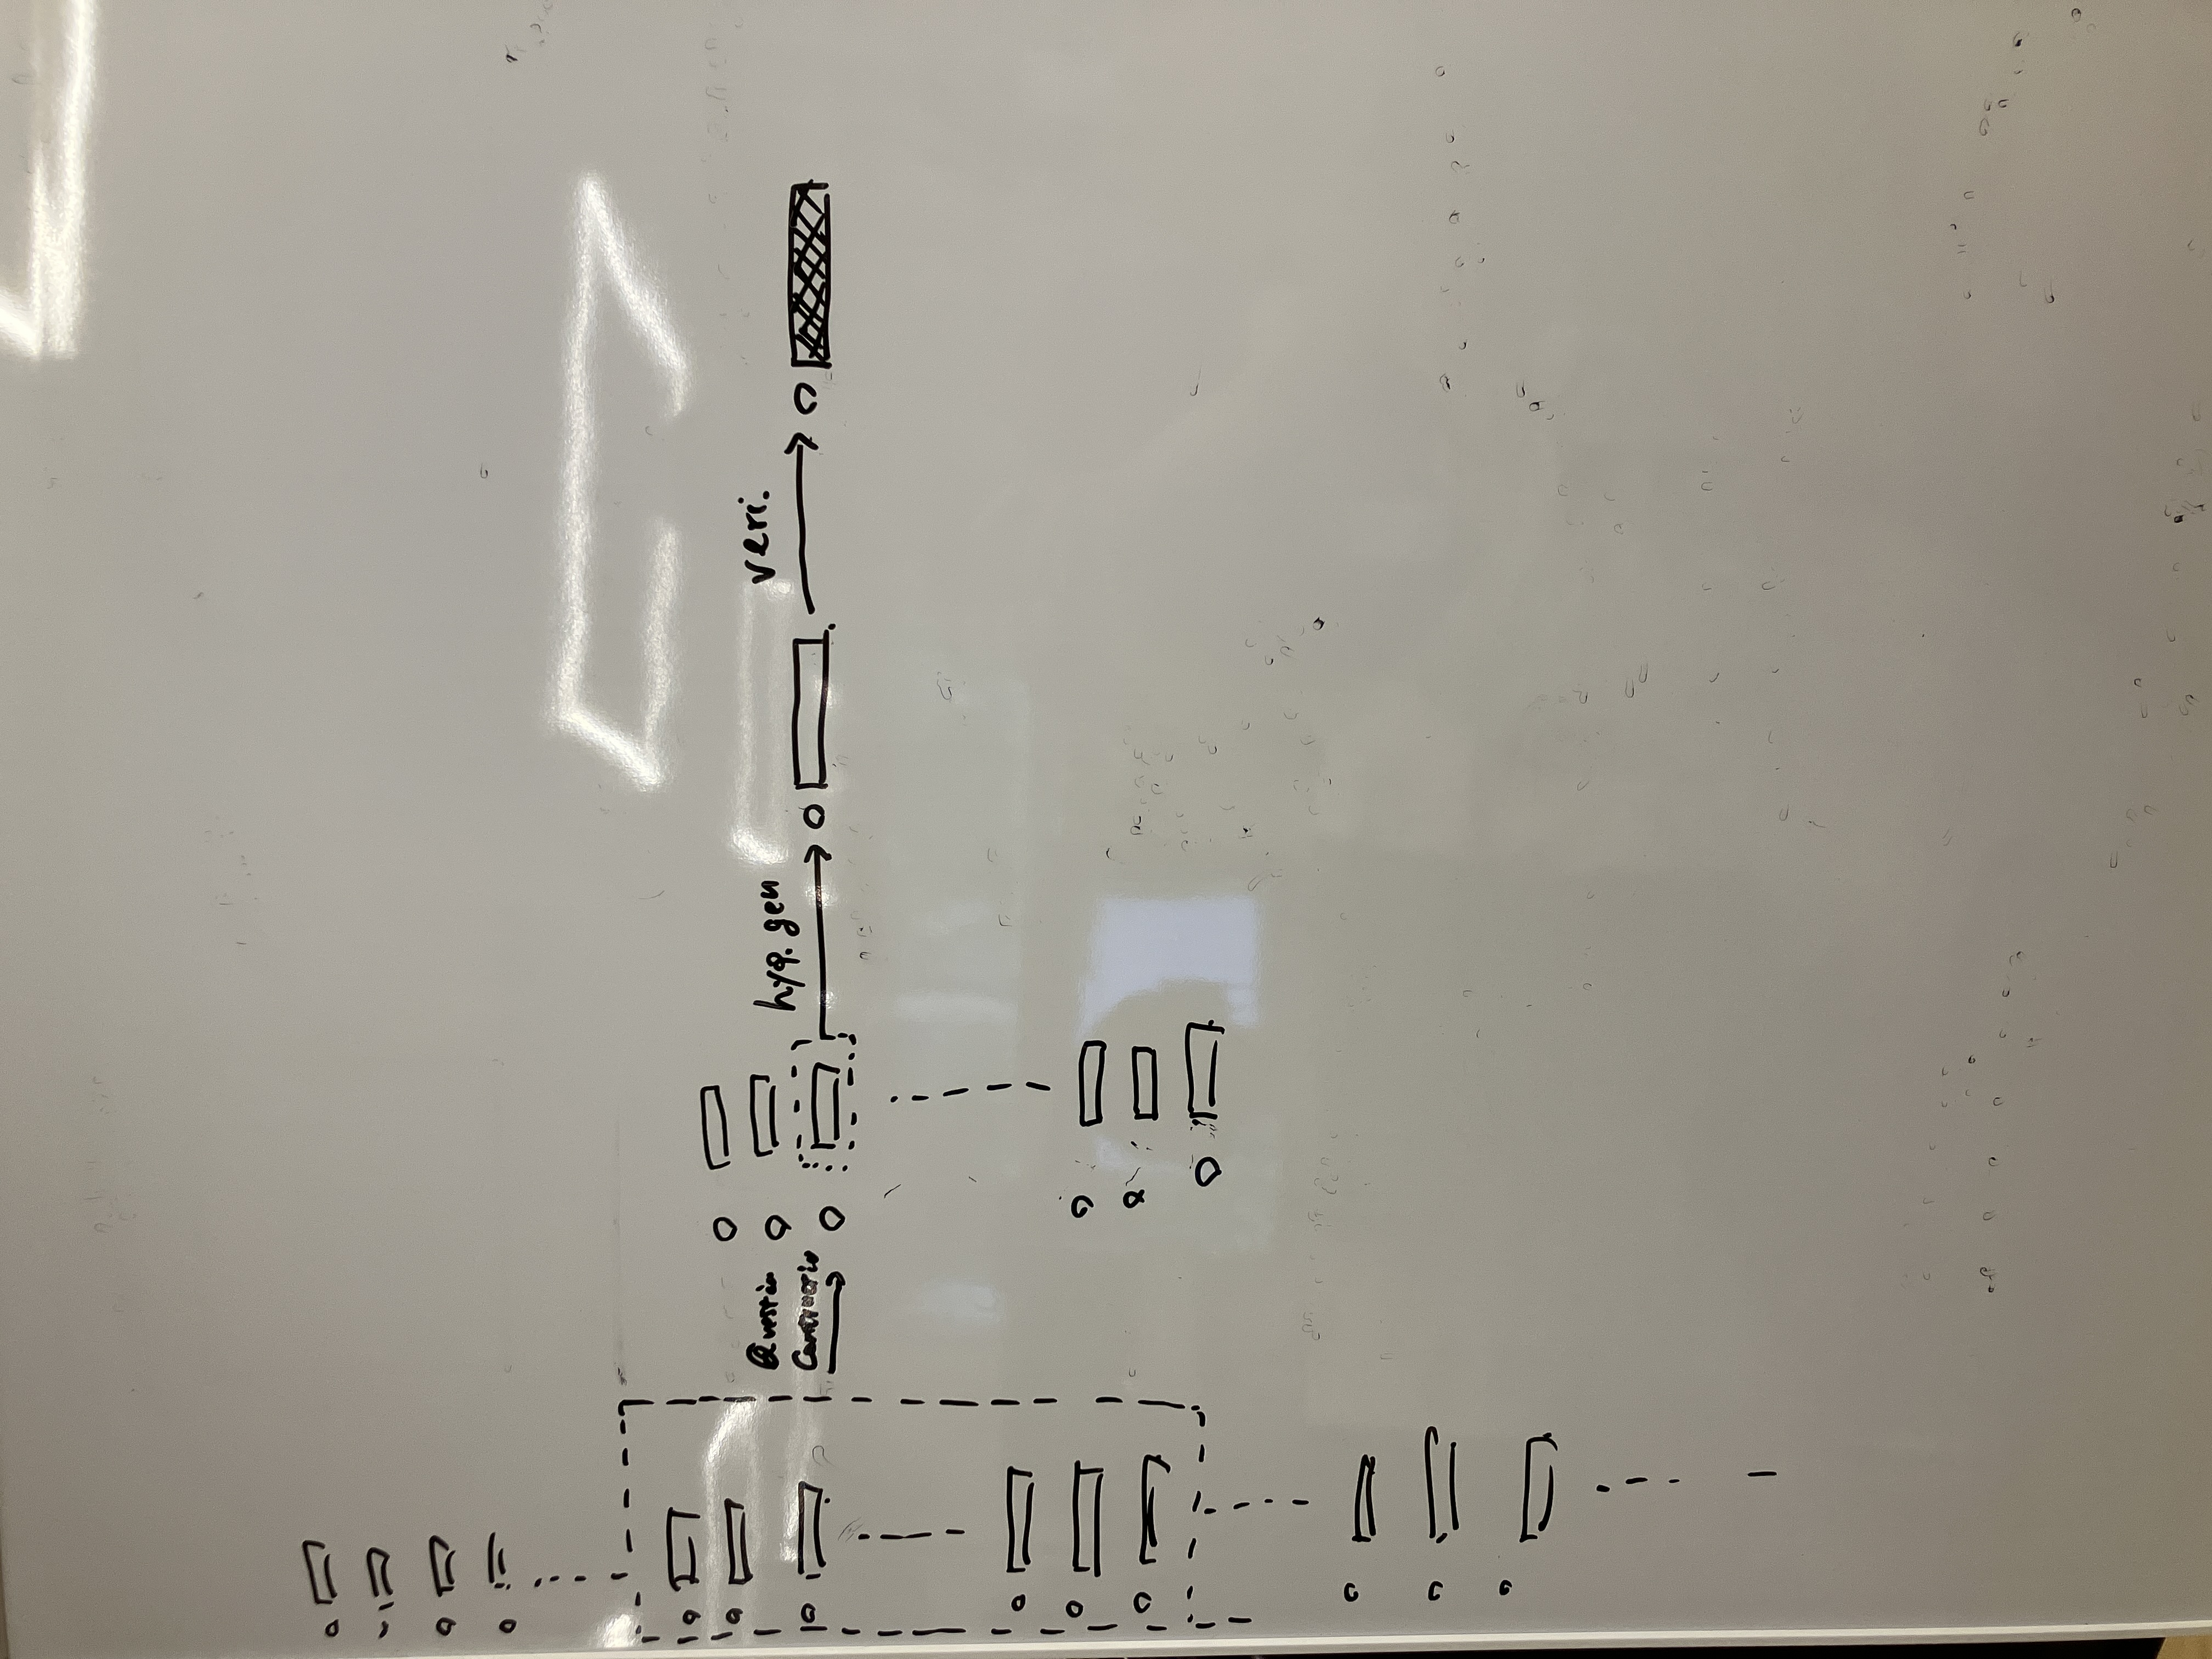
\includegraphics[width=\textwidth]{figs/beliefupdate.jpg}
    \caption{Research Process as Belief Update}
    \label{fig:beliefupdate}
\end{figure}
In the diagram, circles represent statements, and squares represent beliefs in response to those statements. Note that while circles were described as statements, they are not limited to textual representations as long as they are associated with beliefs. Beliefs are determined by the subject holding the belief (in this case, an agent) and the object of the belief (the statement), but please note that I are assuming a fixed agent in this context.

Firstly, in this world, there exist countless pairs of statements and corresponding beliefs (or latent beliefs). Posing a question corresponds to extracting a subset of unknown statements from this pool. More precisely, an unknown statement refers to a statement for which the agent is unsure whether to assign a strong or weak belief. Choosing corresponds to implicitly determining a function that assigns beliefs to each statement. For example, let's consider posing the question ``When did the universe begin?'' This answer to this question is unknown to humanity. By posing this question, the range of possible answers is narrowed down. However, it is not realistically possible for an agent to be aware of all statements and potential answers that could exist. Therefore, while I mentioned pairs of beliefs and statements, please consider that most of these beliefs are latent and potential.

Next, generating a hypothesis involves selecting one pair of a claim and a belief from among the potential claims that could serve as potential answers to the question. It is at this point, by choosing a hypothesis or considering multiple candidate hypotheses, that discourse becomes consciously acknowledged, and beliefs are substantively assigned. Finally, as I discussed in Chapter 2, verification involves gaining evidence for the belief in the chosen hypothesis, resulting in the updating of the belief state. The updated beliefs are represented in black in the diagram.


\end{document}